\documentclass[12pt]{article}

\usepackage{textcomp}
\usepackage[cm]{fullpage}
\usepackage{amsfonts}
\usepackage{verbatim}
\usepackage[english]{babel}
\usepackage{pifont}
\usepackage{color}
\usepackage{setspace}
\usepackage{lscape}
\usepackage{indentfirst}
\usepackage[normalem]{ulem}
\usepackage{booktabs}
% \usepackage{nag}
\usepackage[backend=biber,style=authoryear,maxbibnames=9,maxcitenames=2,uniquelist=false,doi=false,url=false,eprint=false]{biblatex}
\usepackage{float}
\usepackage{latexsym}
\usepackage{hyperref}
\usepackage{url}
% \usepackage{html}
\usepackage{epsfig}
\usepackage{graphicx}
\usepackage{amssymb}
\usepackage{amsmath}
\usepackage{bm}
\usepackage{array}
%\usepackage{mhchem}
\usepackage{ifthen}
\usepackage{caption}
\usepackage{xcolor}
\usepackage{amsthm}
\usepackage{amstext}
\usepackage{nicefrac}
\usepackage{algorithm}
\usepackage{algorithmic}
\usepackage[scientific-notation=true]{siunitx}
\usepackage{subfigure}
\usepackage[flushleft]{threeparttable}
\usepackage{lineno}
\usepackage{adjustbox}
\usepackage{ragged2e}
\usepackage{authblk}
\usepackage{multirow}
\usepackage[T1]{fontenc}
\usepackage{lmodern}
\usepackage{beramono}
\usepackage{tcolorbox}
\usepackage{soul}

\setuldepth{after}
\setlength{\parskip}{1em}
\renewcommand{\baselinestretch}{2.0}
\renewcommand\Affilfont{\small}

\makeatletter
\def\verbatim@font{\linespread{1}\tiny\ttfamily}
\makeatother

\addbibresource{StarBEAST2-refs.bib}

\begin{document}

\title{StarBEAST2 v15 tutorial}
\author[1]{Huw A. Ogilvie\thanks{huw.a.ogilvie@rice.edu}}
\affil[1]{Department of Computer Science, Rice University, Houston, Texas}

\maketitle

\clearpage

\section{Introduction}
\label{sec:intro}

StarBEAST2 is a method for multilocus, multispecies coalescent phylogenetic
inference \parencite{Ogilvie2017}. Multilocus methods like StarBEAST2 take as
input one or more multiple sequence alignments derived from genomic loci.
There is assumed to be no recombination within each locus and free
recombination between loci. Therefore the sequence alignments should be
relatively short, and relatively distantly spaced along the genome. Genomic
data sets which are typically a good fit to the StarBEAST2 model include
RAD-seq loci \parencite{Ogilvie2016} or exons \parencite{Scornavacca2017}.

StarBEAST2 can be used to estimate species tree topologies and divergence
times, the topologies and coalescence times of gene trees, the substitution
model rates and base frequencies for those gene trees, per-species population
sizes and per-species molecular clock rates.

Newer versions of StarBEAST2 supports the integration of molecular sequences
and morphological characters for so-called ``total evidence'' analyses, and
the use of fossil data for tip-dating. Fossil data can include ancient DNA,
morphological characters, and the estimated ages of fossils. Tip-dating
calibrates the trees in absolute time, typically millions of years.

This tutorial will cover using StarBEAST2 to estimate a species tree including
per-species population sizes of the genus \textit{Canis} from exon sequences
(Section~\ref{sec:speciesTree}),
to estimate per-species molecular clock rates
(Section~\ref{sec:relaxedClock}),
and to conduct a total evidence tip-dating study
(Section~\ref{sec:FBD}).

\section{Preliminaries}
\label{sec:prelim}

Before doing anything, we need to install StarBEAST2, which is available as a package for
the phylogenetic software platform BEAST2. If you have not yet installed BEAST2,
or if you have an older version, you can download the latest version from \url{http://beast2.org}.
Make sure you have the latest version before proceeding.

After downloading and installing BEAST2 on your computer, open BEAUti ---
the graphical user interface for BEAST2. To install StarBEAST2 (or
any BEAST2 package), open the File menu and select Manage Packages (Figure~\ref{fig:managePackages}).

\begin{figure}[htb!]
\centering
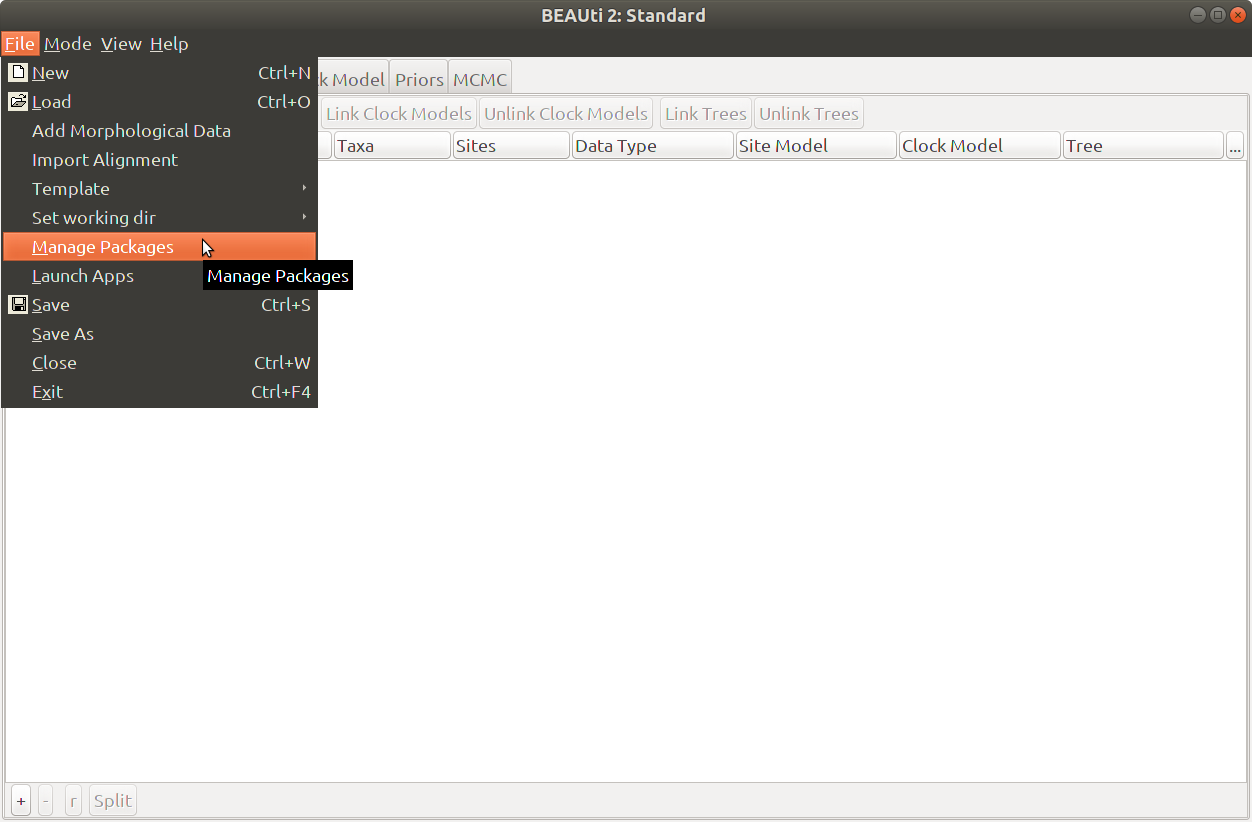
\includegraphics[width=0.8\textwidth]{figures/managePackages.png}
\caption
{Opening the package manager}
\label{fig:managePackages}
\end{figure}

Select StarBEAST2 from the list of available packages and click the install button, which will take
care of the installation for you (Figure~\ref{fig:installStarBEAST2}). After the installation of StarBEAST2 is finished, just like for any BEAST2 package, you
\textbf{must} quit and relaunch BEAUti.

\begin{figure}[htb!]
\centering
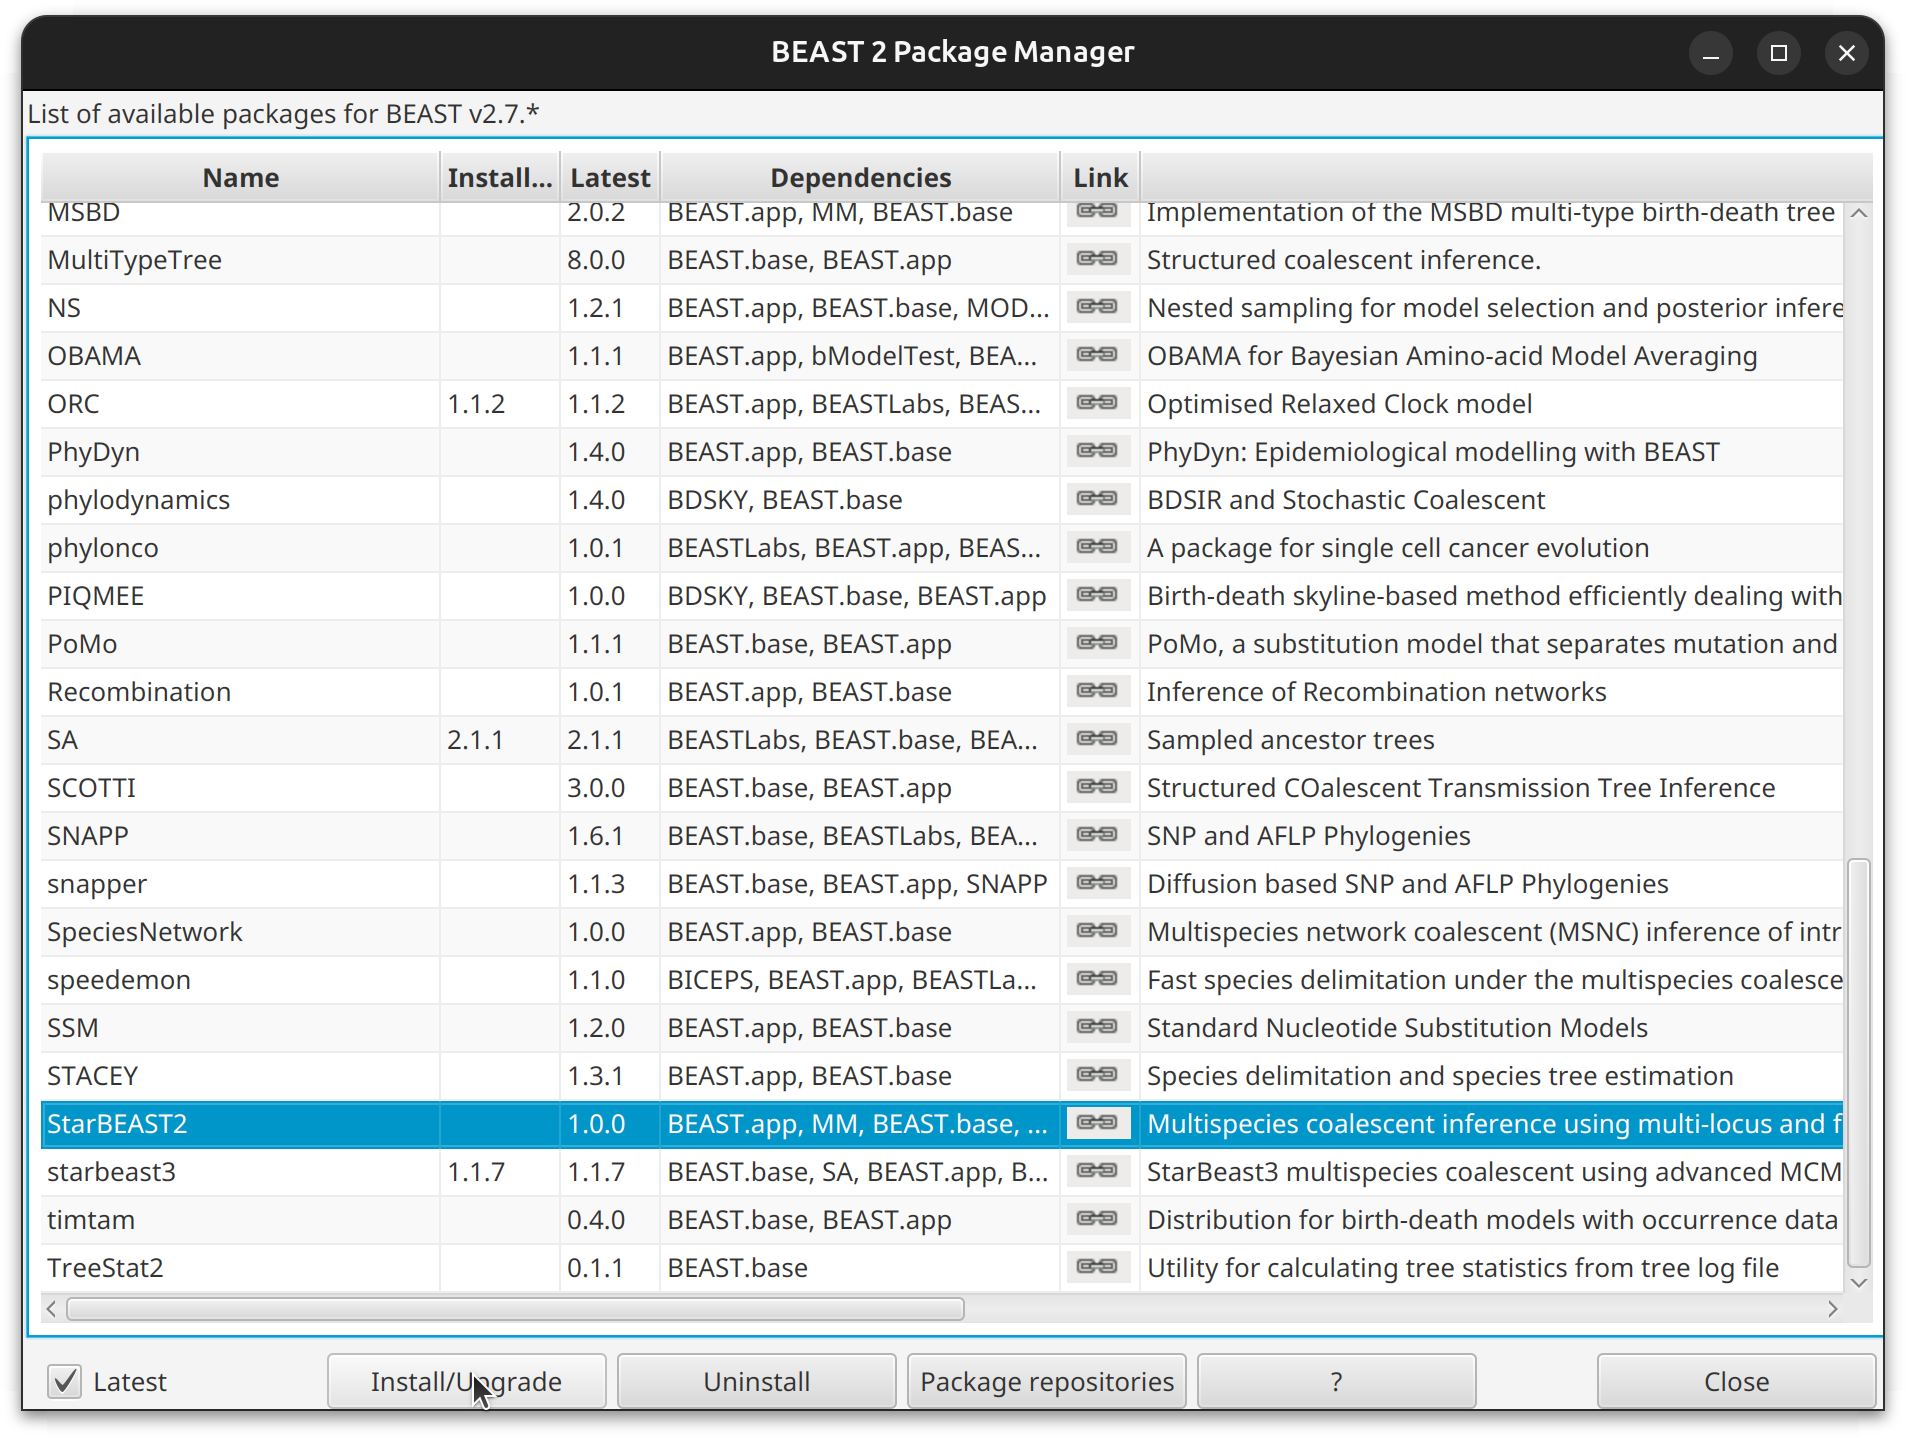
\includegraphics[width=0.8\textwidth]{figures/installStarBEAST2.png}
\caption
{Installing StarBEAST2}
\label{fig:installStarBEAST2}
\end{figure}

After relaunching BEAUti, you will notice four new templates (Figure~\ref{fig:strictClockTemplate}). The first
is ``StarBeast2'', which is for a strict molecular clock or relaxed
gene tree clocks uncorrelated with the species tree lineages. The others
are ``SpeciesTreeUCLN'', ``SpeciesTreeRLC'' and ``SpeciesTreeUCED'' which
enable per-species clock rates, as described by \cite{Ogilvie2016}.
The relaxed clock models used by those templates are uncorrelated log-normal (UCLN),
relaxed local clock (RLC), and uncorrelated exponential distribution (UCED)
respectively.

\begin{figure}[htb!]
\centering
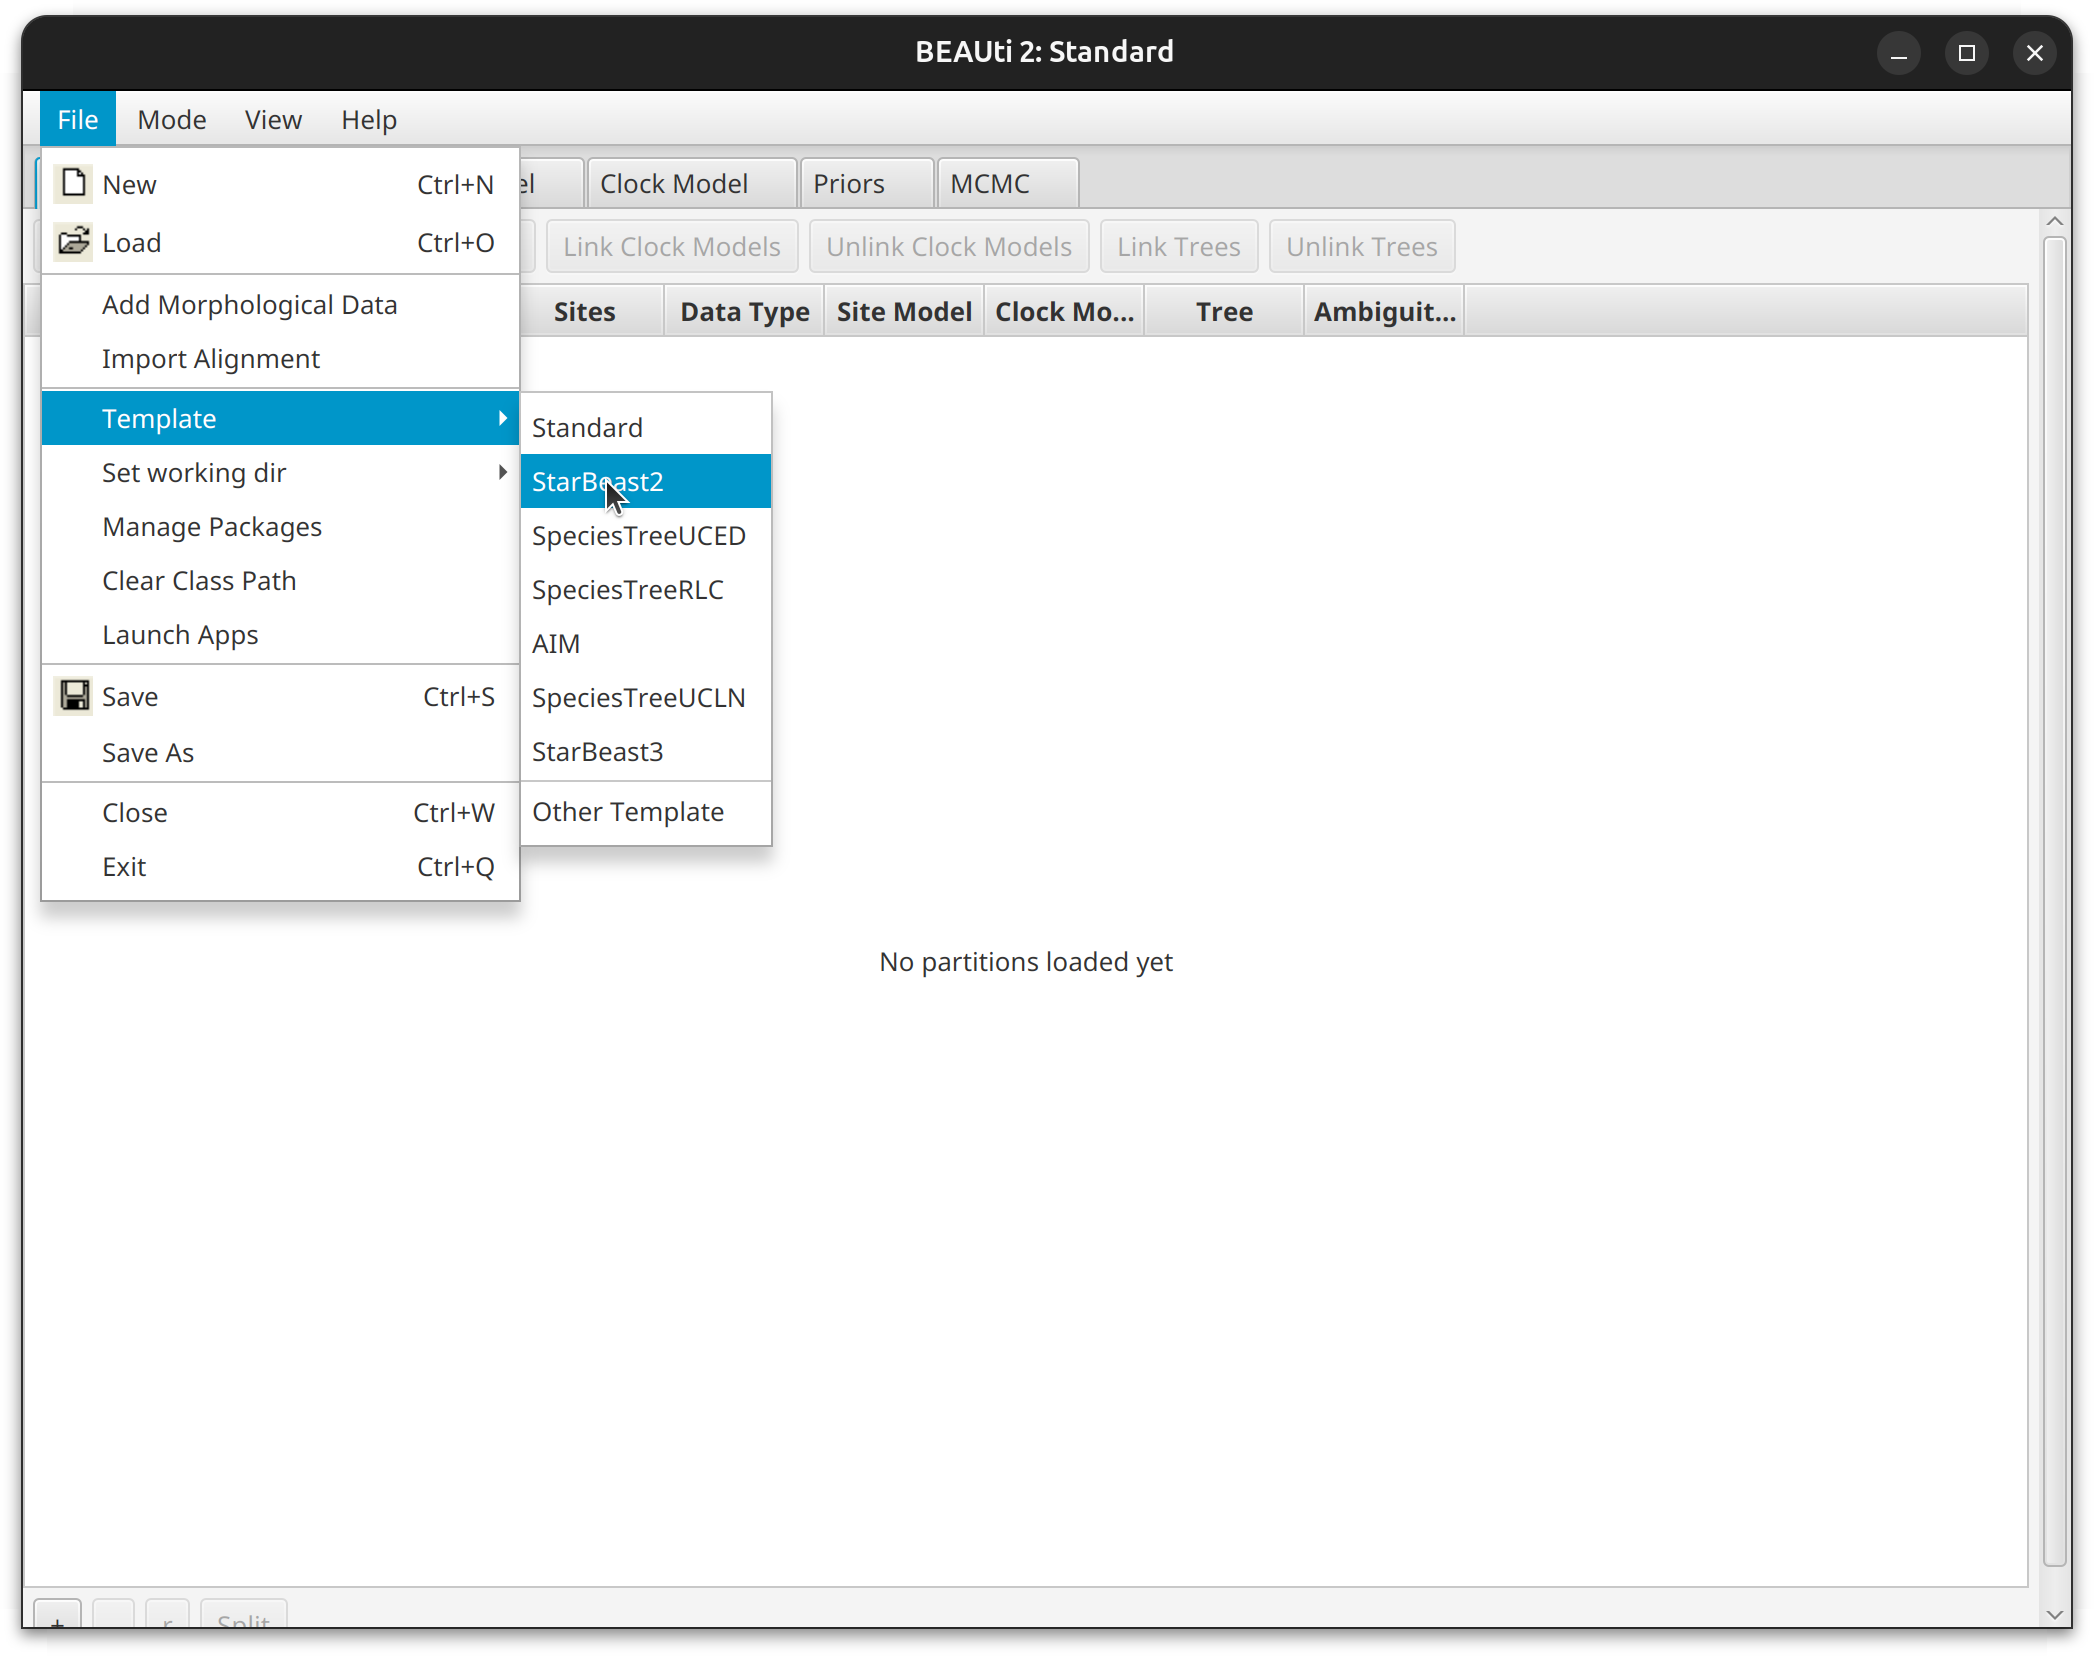
\includegraphics[width=0.8\textwidth]{figures/strictClockTemplate.png}
\caption
{Selecting a StarBEAST2 template}
\label{fig:strictClockTemplate}
\end{figure}

To visualize posterior distributions of trees, we will be using DensiTree
\parencite{Bouckaert2010} which is included with BEAST2. We will also use
FigTree to view summary trees, and Tracer to check on parameters and
statistics. FigTree is available from \url{http://tree.bio.ed.ac.uk/software/figtree/}
and Tracer from \url{http://tree.bio.ed.ac.uk/software/tracer}. Please make sure both are
installed before proceeding.

\clearpage

\section{Reconstructing the species tree of \textit{Canis}}
\label{sec:speciesTree}

The genus \textit{Canis} includes species such as \textit{Canis lupus} (wolves),
\textit{Canis latrans} (coyotes), and \textit{Canis dirus} (dire wolves, extinct).
Because the
taxonomy of this genus is quite messy, it also includes
\textit{Cuon alpinus} and \textit{Lycaon pictus}.
In this section we will reconstruct the species tree of \textit{Canis} using StarBEAST2.

\subsection{Importing alignments}
\label{subsec:importingAlignments}

First up, create a new folder somewhere with a sensible name like
``CanisPhylogeny''. Relaunch BEAUti and load up the strict clock
template by selecting ``StarBeast2'' from the Templates submenu of the File menu
(Figure~\ref{fig:strictClockTemplate}). Now we will import multiple sequence
alignments of the 16 nuclear loci sequenced by \cite{LindbladToh2005}. Select
Import Alignments from the File menu, and navigate to the ``data'' subfolder
of the tutorial. Select all 16 FASTA files, and click OK to import
(Figure~\ref{fig:fastaFileImport}). Do not select ``morphology-canis.nexus''
which is for the total evidence study.

\begin{figure}[htb!]
\centering
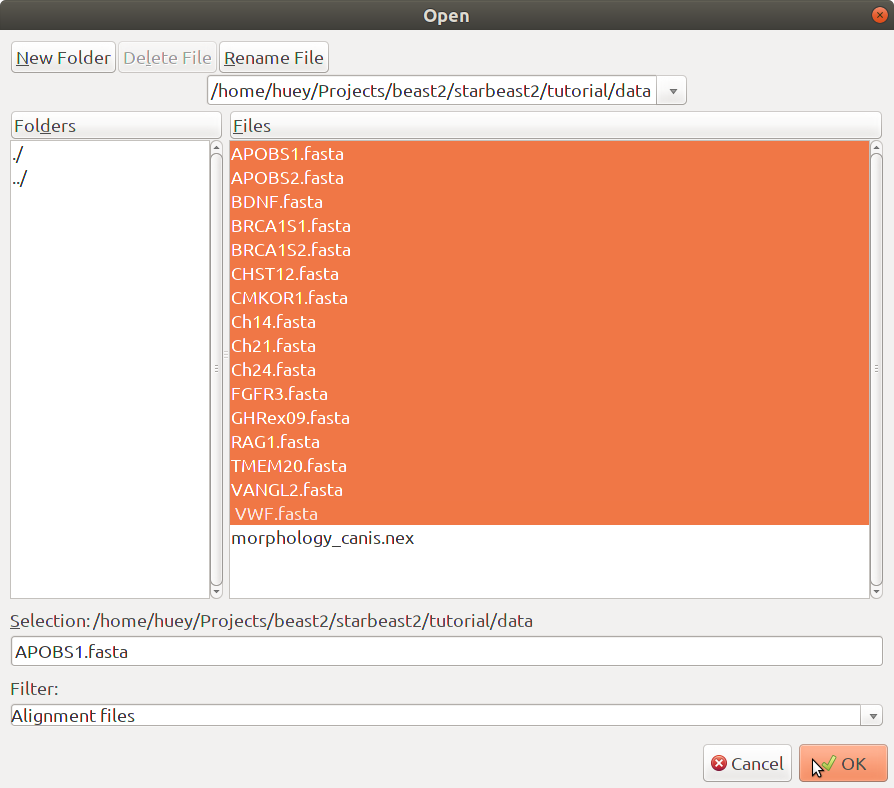
\includegraphics[width=0.7\textwidth]{figures/fastaFileImport.png}
\caption
{Importing \textit{Canis} multiple sequence alignments}
\label{fig:fastaFileImport}
\end{figure}

After you click OK, you will be asked what type of sequences are in the files.
As all 16 files are MSAs of nucleotide sequences, select ``all are nucleotide''
and click OK again to continue. There should now be 16 partitions listed in
BEAUti.

\clearpage

\subsection{Linking models}
\label{subsec:linkingModels}

As a general rule, clock models should be linked when using the strict clock StarBEAST2 template. Rates between
loci are still allowed to vary and the mean rate among all sites is fixed at 1. Therefore
by linking the clocks, the average clock rate can be fixed at an \textit{a priori} value
to calibrate the analysis, or estimated when node-dating or tip-dating is used.
Select all 16 loci and click the ``Link Clock Models'' button. Now all loci
should have ``APOBS1'' as the clock model name. The site model, clock model and tree names are text fields that you can click on to edit. Change the name of the clock model to ``molecular'' and it should look like Figure~\ref{fig:linkModels}.

\begin{figure}[htb!]
\centering
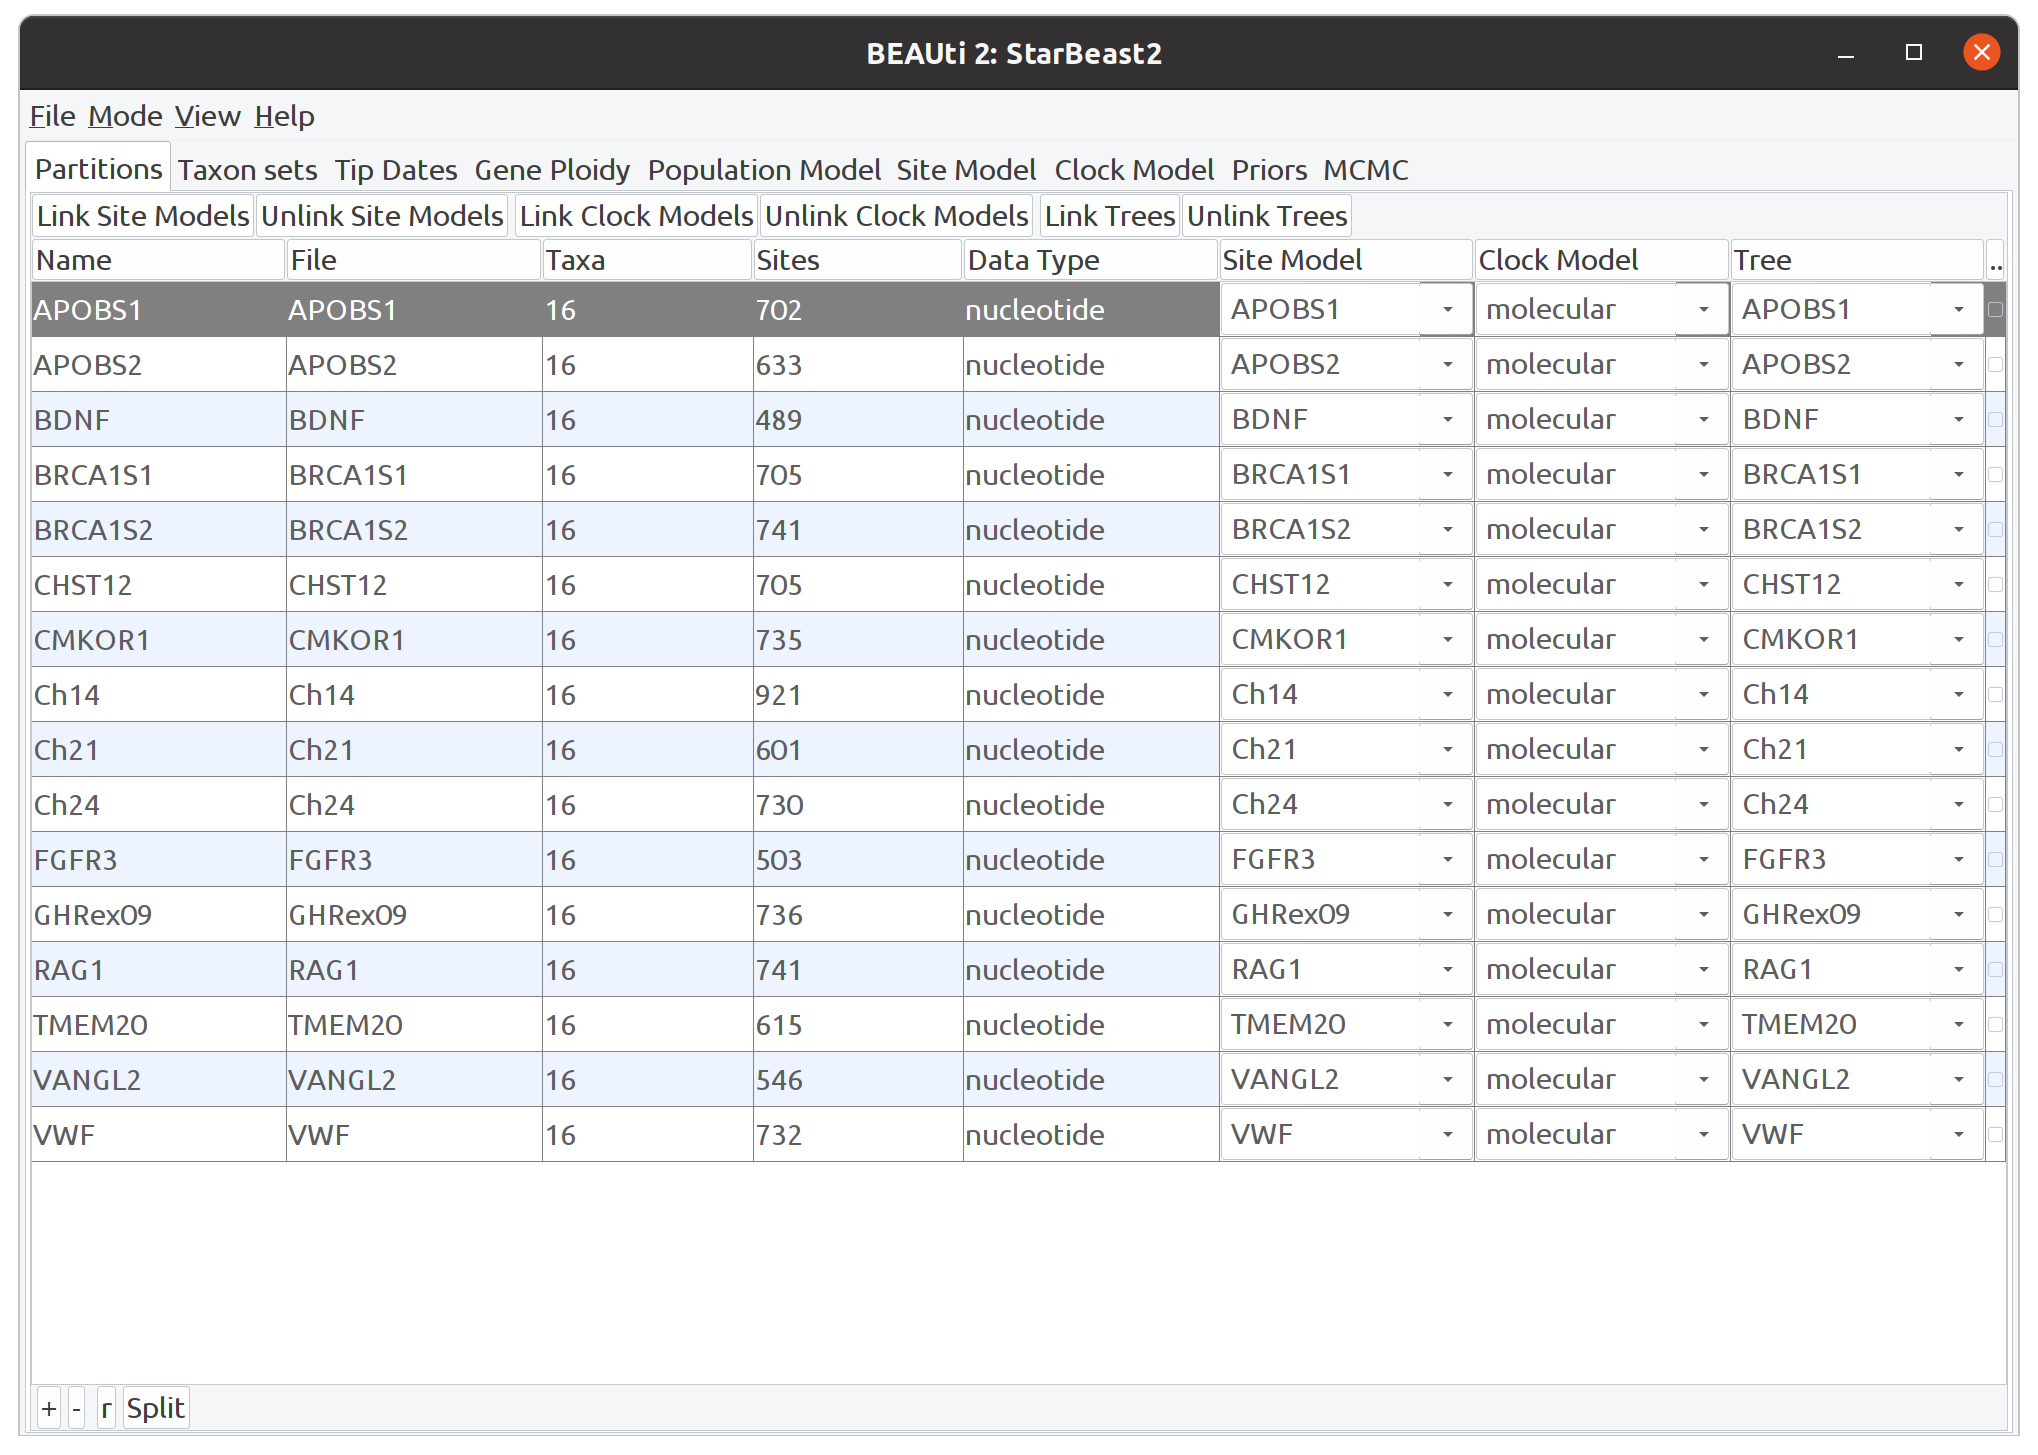
\includegraphics[width=0.8\textwidth]{figures/linkModels.png}
\caption
{Linking clock models}
\label{fig:linkModels}
\end{figure}

\clearpage{}

\begin{tcolorbox}[colback=green!5,colframe=green!40!black,title=Mixing nuclear and mitochondrial loci]
StarBEAST2 can be used with a combination of mitochondrial and nuclear loci, but this requires careful thought when specifying the model. One possibility is to link the nuclear loci as above, but not to link the mitochondrial loci. Then when editing the site models, untick ``estimate'' for the substitution rate of each mitochondrial locus. Now separate clock rates will be used for each mitochondrial locus, in addition to the overall clock rate which applies to nuclear loci.

If the species tree is calibrated using an \textit{a priori} nuclear or mitochondrial molecular clock rate, you can set that rate in the Clock Model panel. If the mitochondrial rate is fixed, the nuclear rate should probably be estimated and \textit{vice versa}. If the species tree is calibrated using node or tip dating, then all clock rates should probably be estimated.

Make sure appropriate priors are used for all estimated clock rates. This could be a $1/X$ prior for rates where you genuinely have no prior knowledge. However in most circumstances you will have a general idea of the clock rate, e.g. within an order of magnitude. In that case, you can set a broad prior with a mean based on your prior knowledge. Broad priors include Log Normal with a large standard deviation (up to about 2), or a Gamma distribution with a small $\alpha$ (set ``alpha'' to 1 or 2).
\end{tcolorbox}

\begin{tcolorbox}[colback=purple!5,colframe=purple!40!black,title=Linking site models]
When clock models are linked as is recommended by this tutorial, linking site models will result in every gene having exactly the same
clock rate. As this is unrealistic, generally site models should \textbf{not}
be linked using BEAUti when setting up a StarBEAST2 analysis.
\end{tcolorbox}

\subsection{Specifying species names}
\label{subsec:speciesNames}

In the FASTA files, each sequence has a name like ``Canis\_anthus\_a''.
Here \textit{Canis anthus} is the binomial name, and ``a'' is a haplotype.
For the data supplied with this tutorial, each species has two haplotypes ``a'' and ``b'', both from
the same diploid individual. However in other studies multiple individuals may
be sequenced, so an arbitrary number of haplotypes are available per species.

To assign haplotypes to species, select the Taxon Sets tab in BEAUti, then
click the Guess button. To assign the correct names, keep ``use everything''
selected, but change ``after first'' to ``before last''. Leave the underscore
in the text box and click OK (Figure~\ref{fig:guessTaxonMap}). This way everything before
the last underscore in the haplotype name will be used as the species name,
so ``Canis\_anthus'' will be the species name for ``Canis\_anthus\_a''.

\begin{figure}[htb!]
\centering
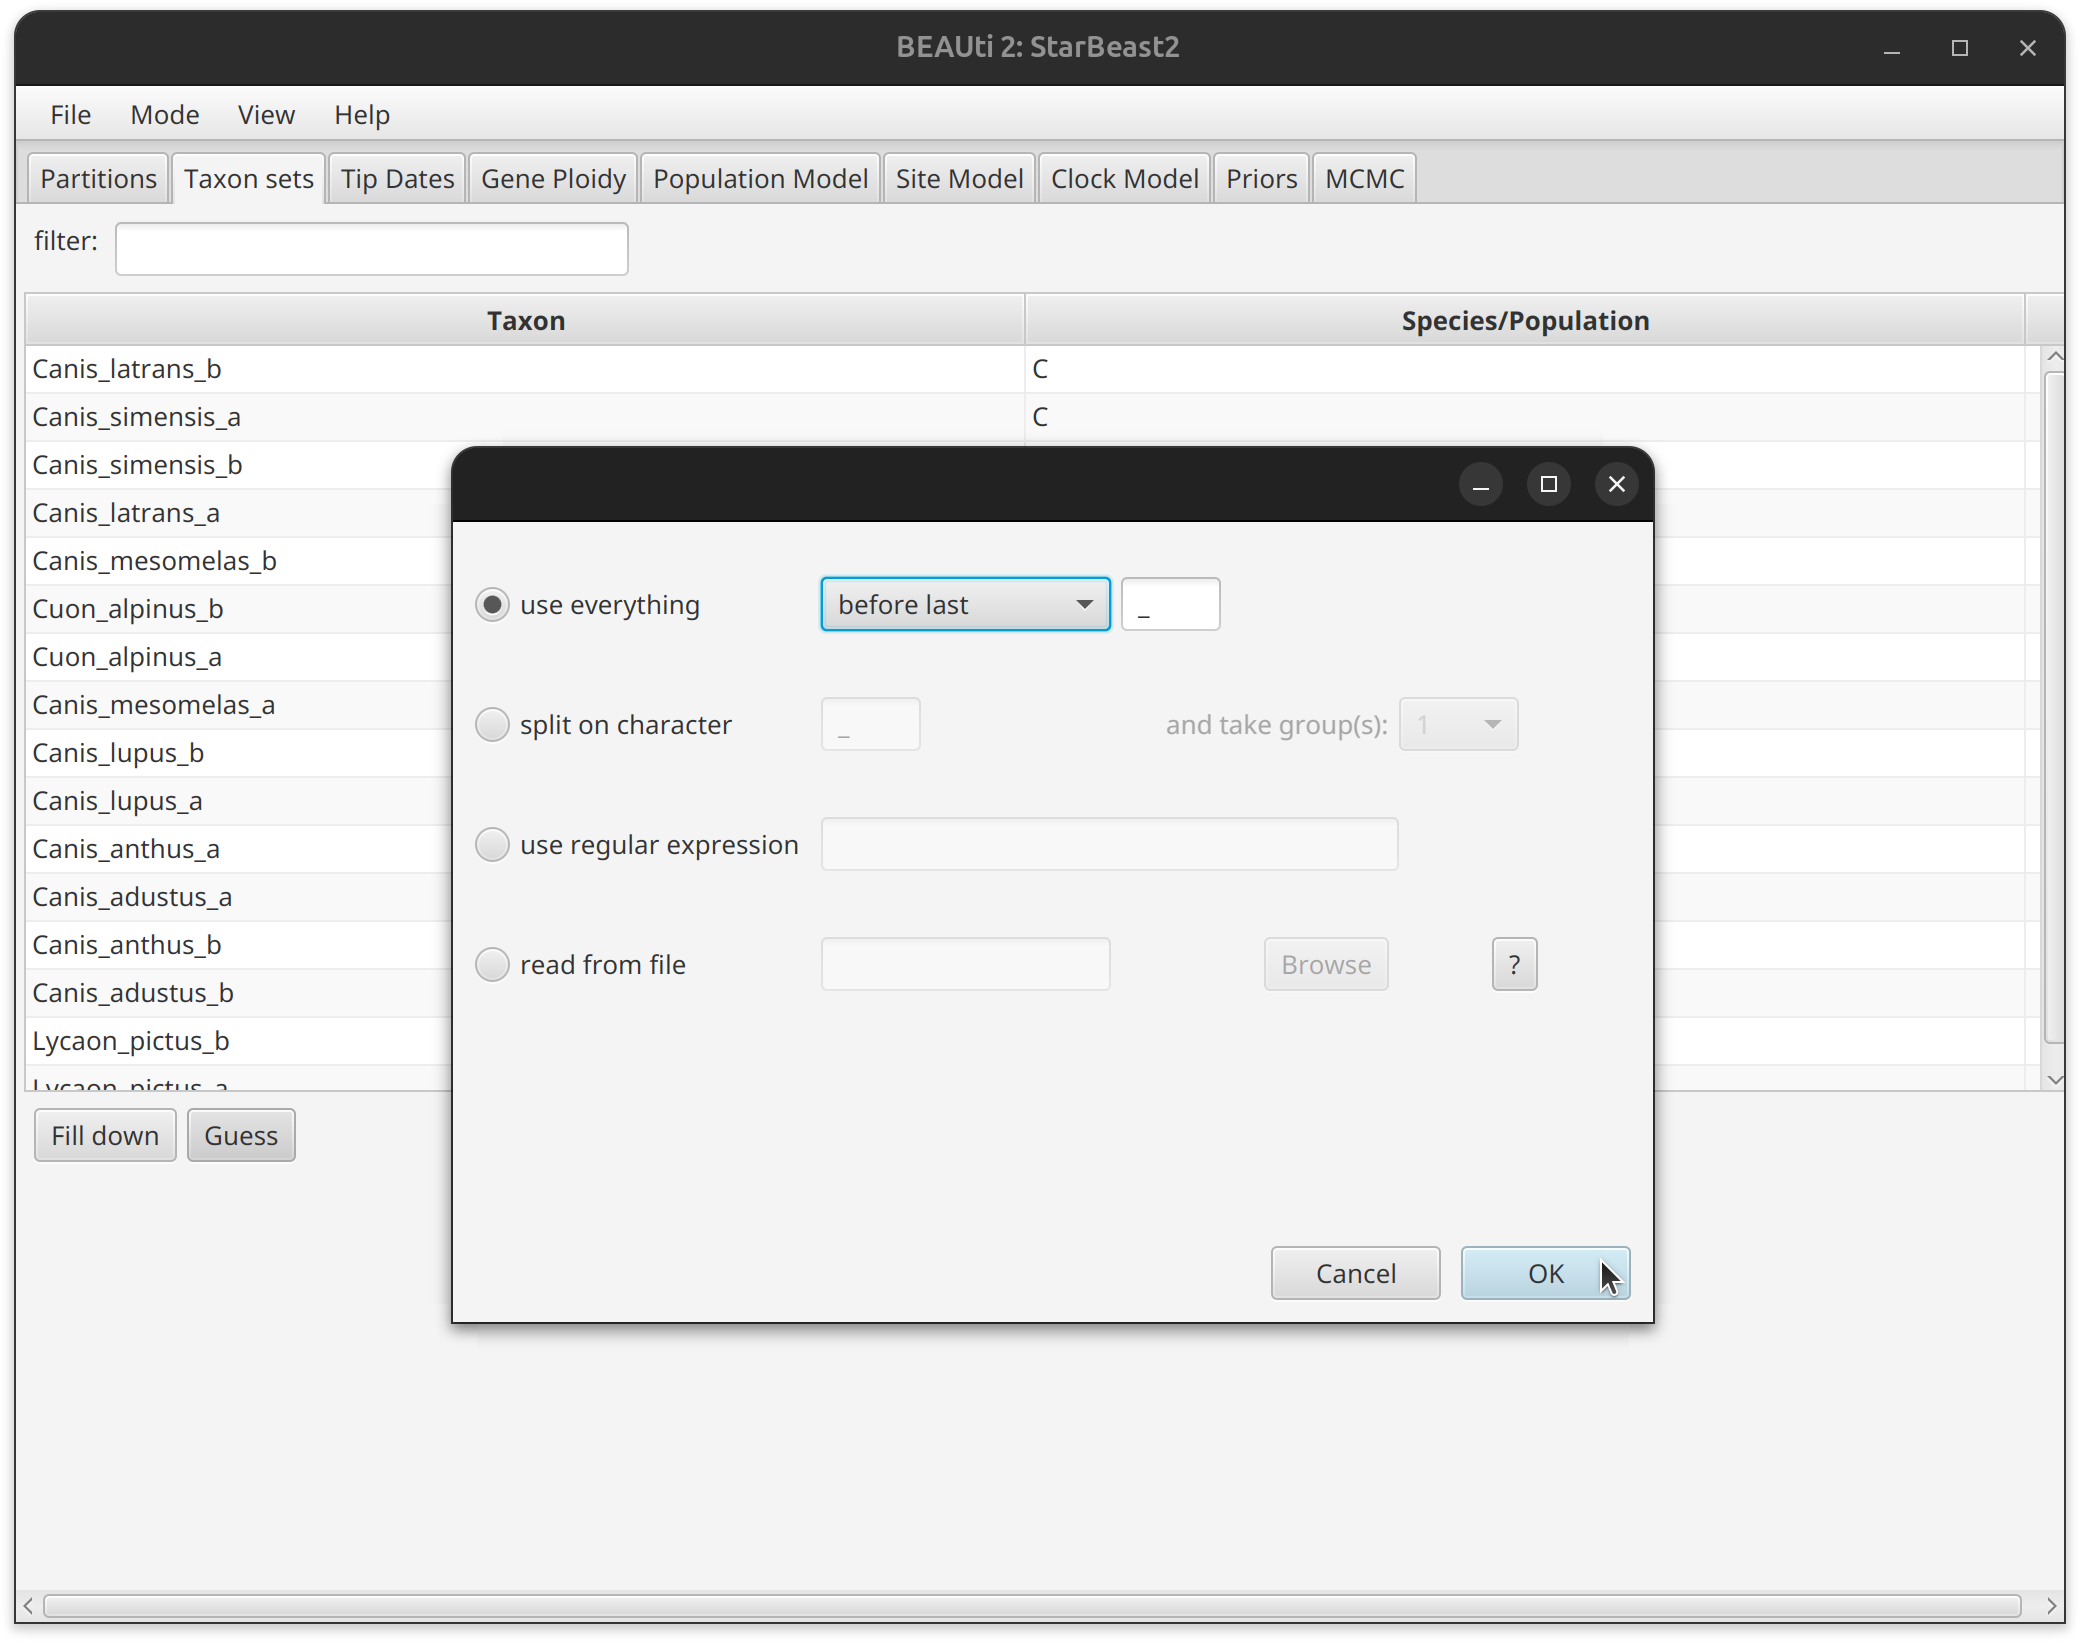
\includegraphics[width=0.4\textwidth]{figures/guessTaxonMap.png}
\caption
{Guessing species names from haplotype names}
\label{fig:guessTaxonMap}
\end{figure}

\newpage{}

Now each haplotype (Taxon) should have a corresponding species (Species/Population).
Based on how we assigned the species names, there should be two haplotypes
``a'' and ``b'' for each species (Figure~\ref{fig:taxonMap}).

\begin{figure}[htb!]
\centering
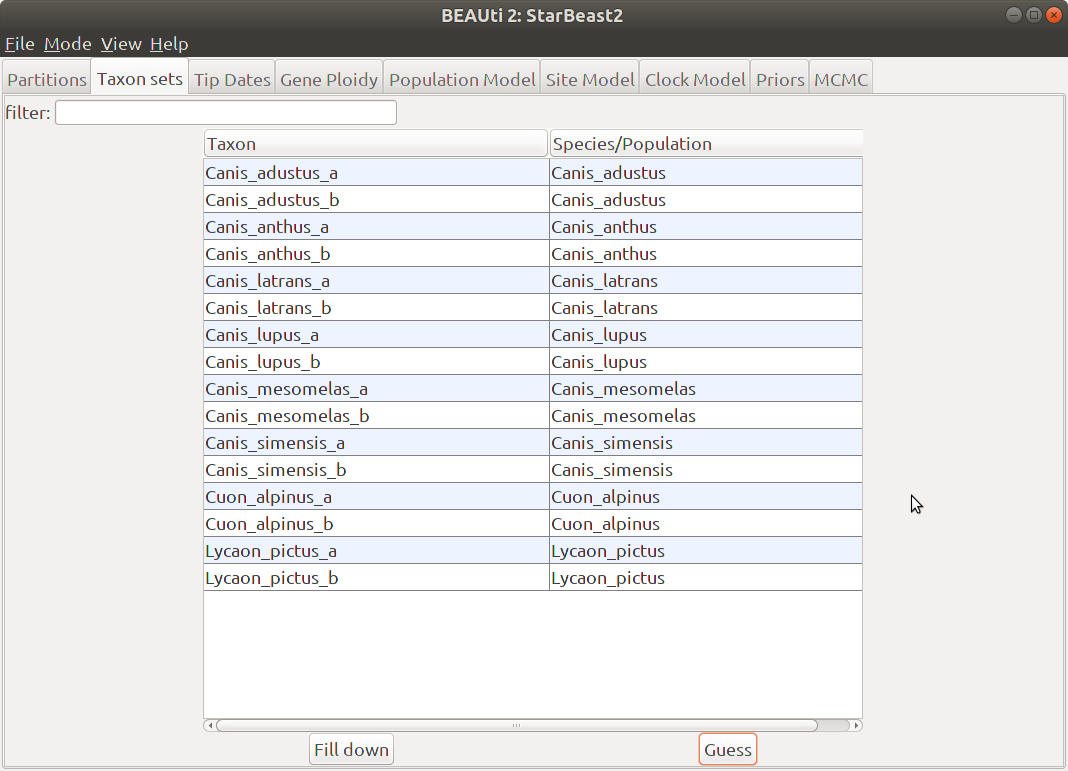
\includegraphics[width=0.8\textwidth]{figures/taxonMap.png}
\caption
{The assignment of haplotypes to species}
\label{fig:taxonMap}
\end{figure}

\clearpage

\subsection{Gene Ploidy and Population Model}
\label{subsec:ploidyAndPopModel}

Ignore the Tip Dates tab, which is for tip-dating and will be covered in
section~\ref{sec:FBD} of the tutorial. Open the Gene Ploidy tab, and observe that the default value
for all loci is 2.0. This is because there are two copies of a locus in each
individual for diploid populations, so we scale the effective population sizes
by 2.0. If you use any mitochondrial or Y/W chromosomal loci, you should
change their ploidy to 0.5, because there is on average only 0.5 copies per
individual. The ploidy of X/Z chromosomal loci should be set to 1.5 for the
same reason.

Select the Population Model tab. By default analytical integration is used,
which is slightly faster but does not produce estimates of per-species population sizes.
Change the model to ``Constant Populations'', which will add effective population
sizes to the species tree output (Figure~\ref{fig:constantPopulations}).

\begin{figure}[htb!]
\centering
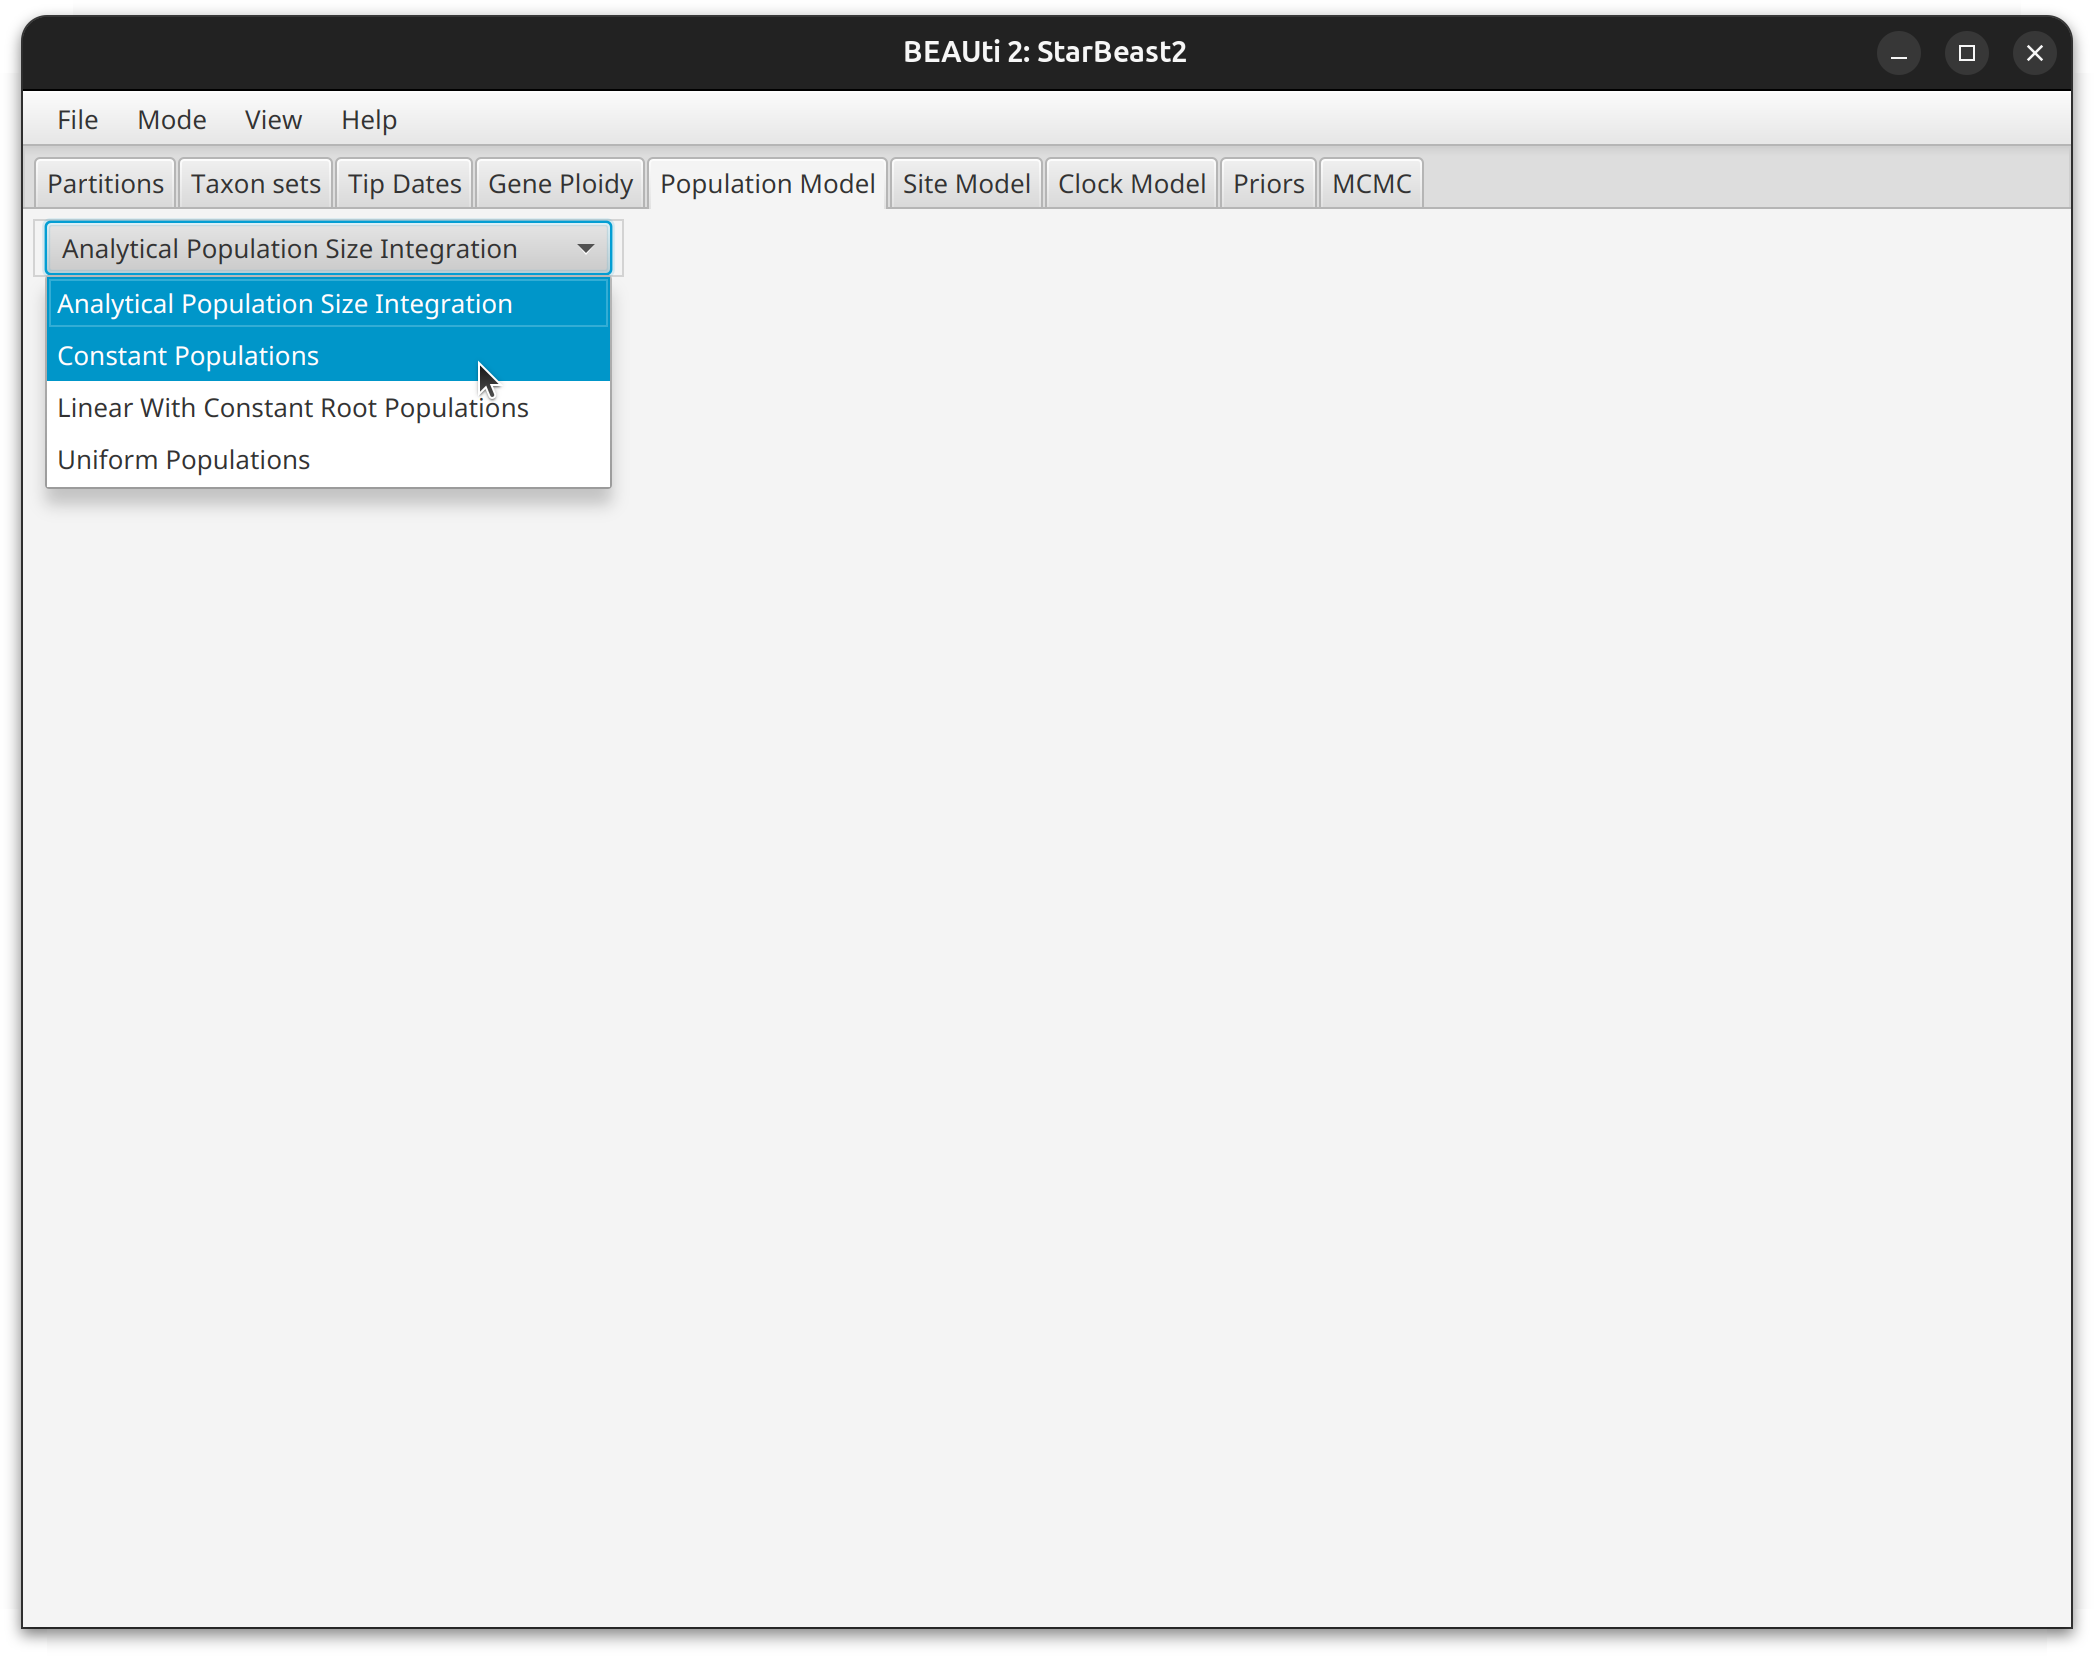
\includegraphics[width=0.8\textwidth]{figures/constantPopulations.png}
\caption
{Changing the population model}
\label{fig:constantPopulations}
\end{figure}

\clearpage

\subsection{Site Model}
\label{subsec:siteModel}

Select the Site Model tab, and you will see the site model for the first partition
displayed. Change ``JC69'' to ``HKY'', and then set the frequencies to
empirical (Figure~\ref{fig:hky}).
HKY is more flexible because it allows nucleotide transitions to have a different
rate relative to transversions \parencite{Hasegawa1985}.

\begin{figure}[htb!]
\centering
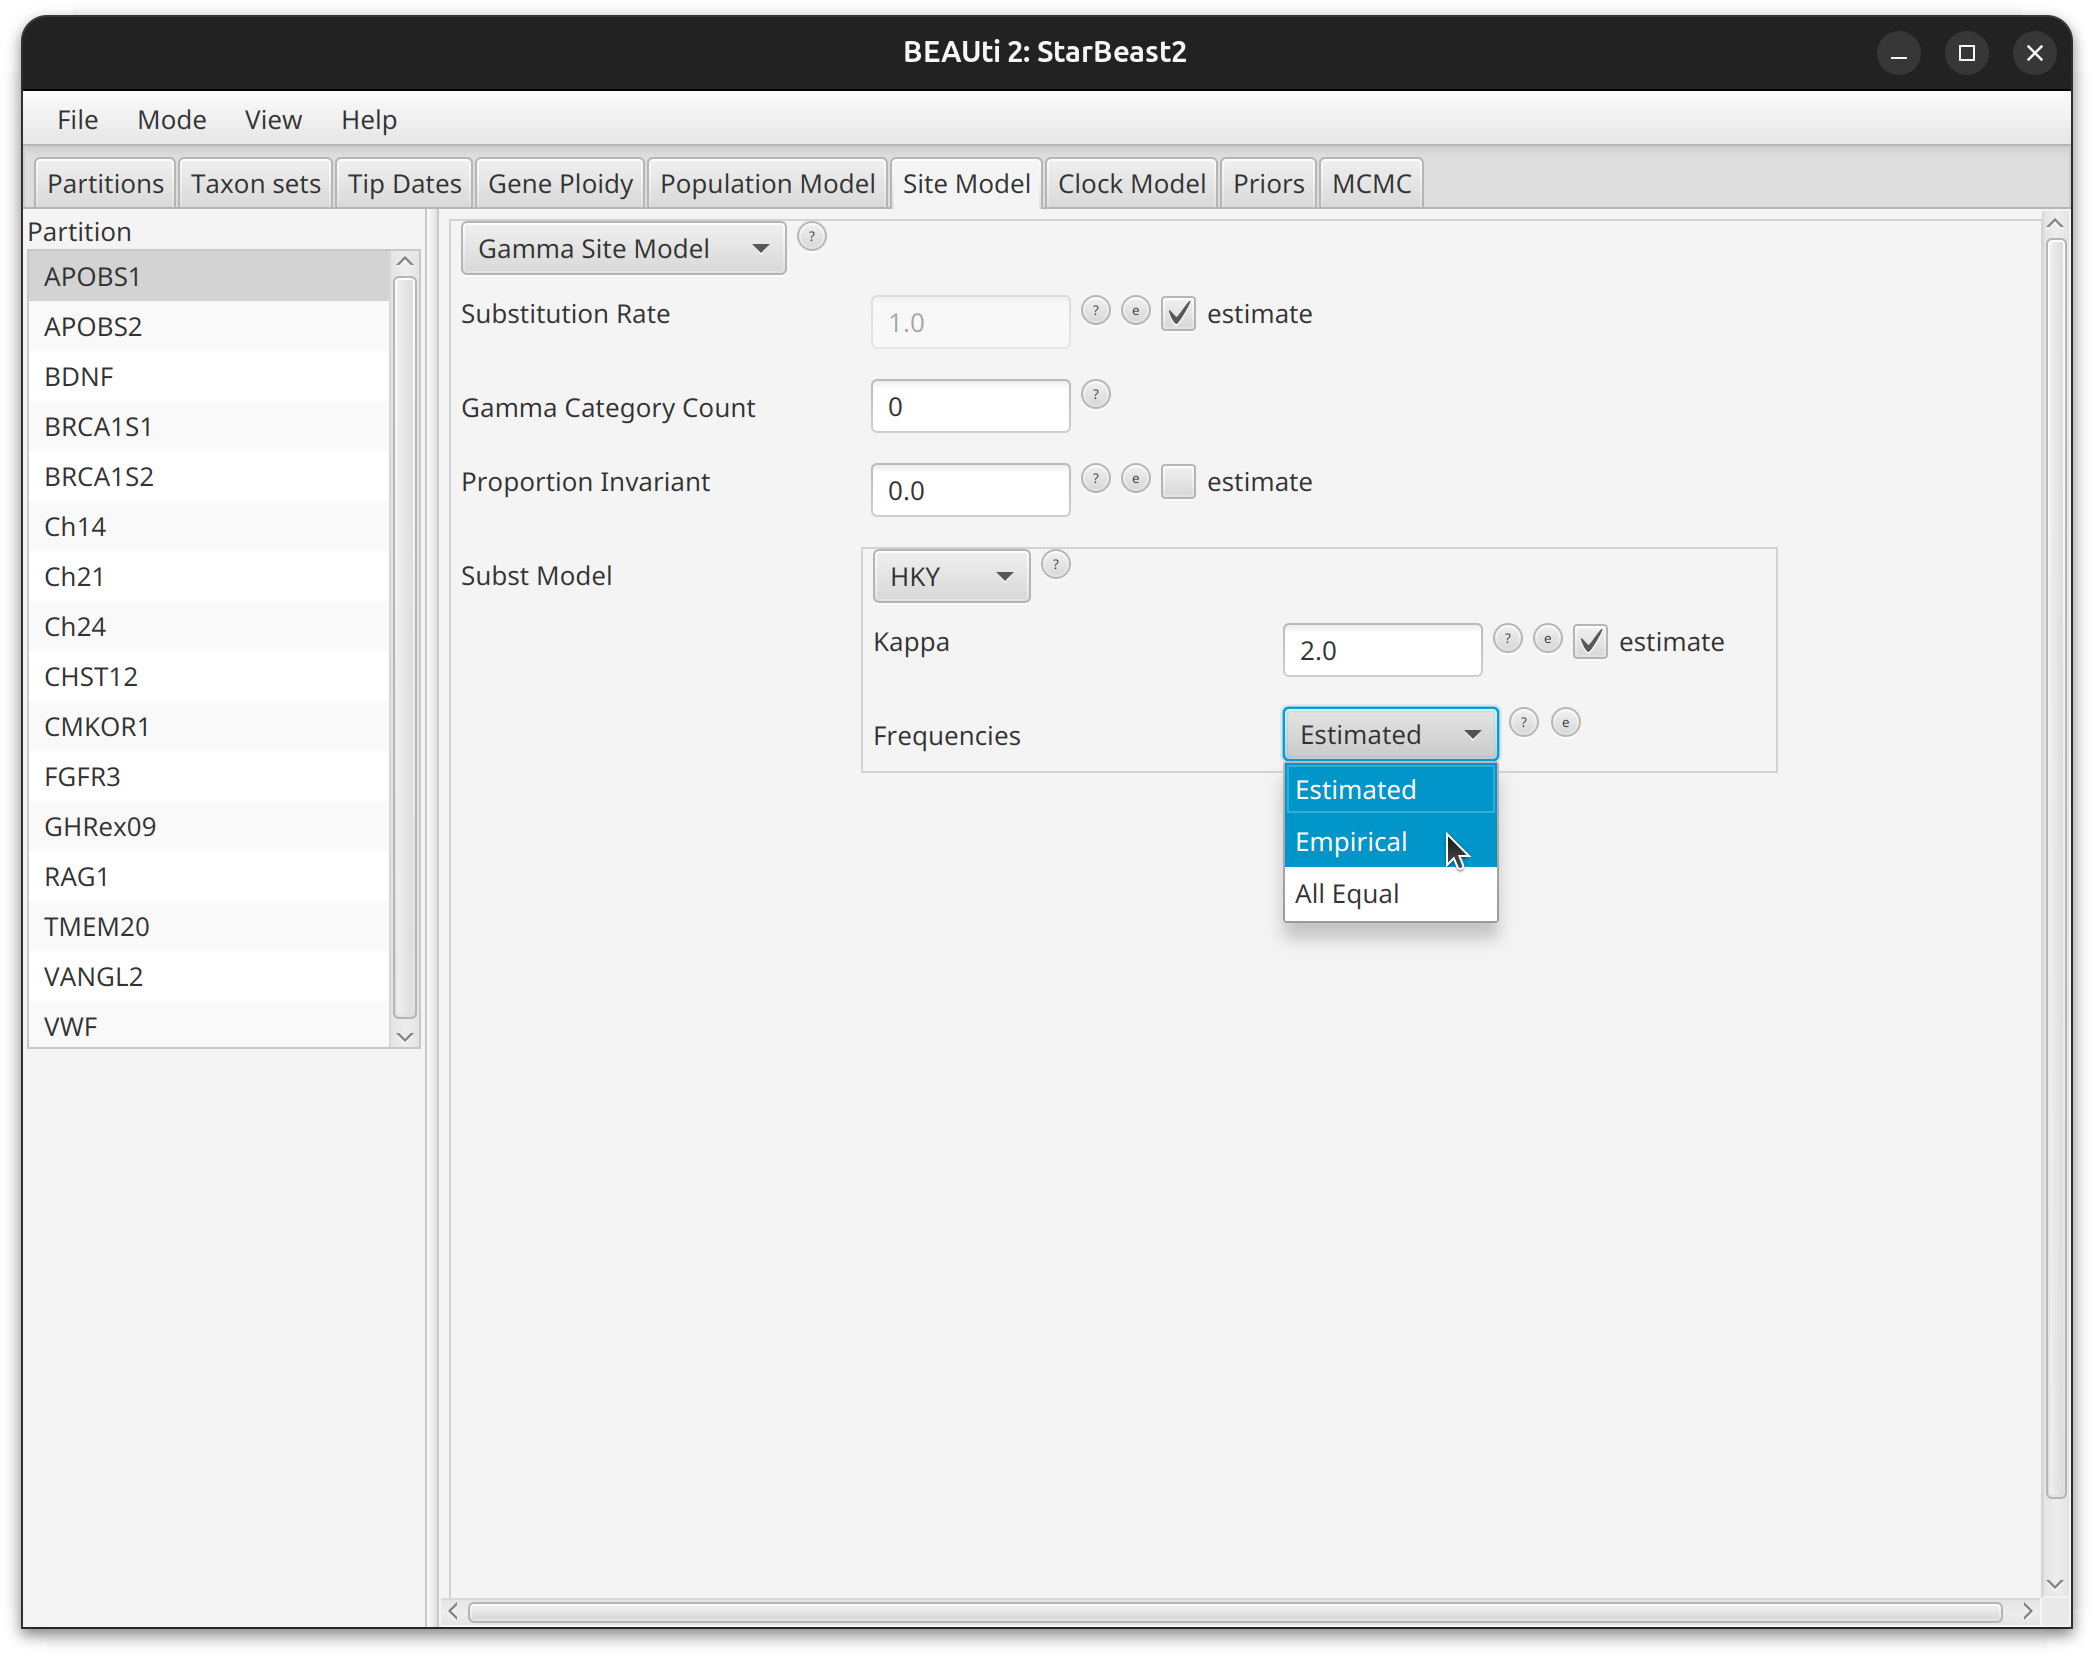
\includegraphics[width=0.8\textwidth]{figures/hky.png}
\caption
{Setting the site model to HKY with empirical base frequencies}
\label{fig:hky}
\end{figure}

Now to change the site model for all loci to HKY with empirical base frequencies,
select all of the partitions in the left hand column with the shift key. Then
click ``OK'' to apply the same site model used for the first locus
to everything else (Figure~\ref{fig:cloneSiteModel}).

\newpage{}

\begin{figure}[htb!]
\centering
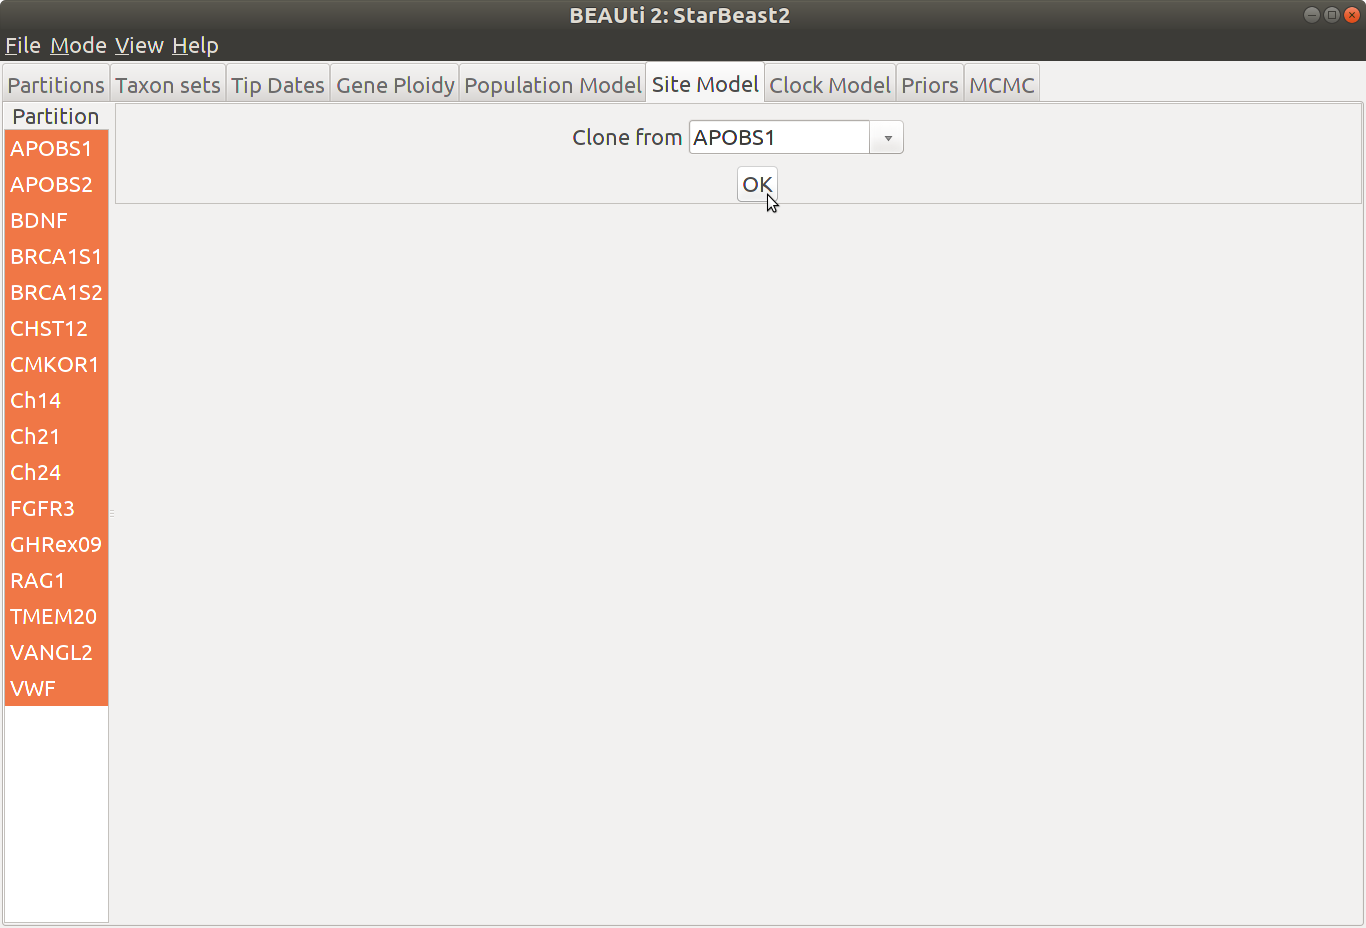
\includegraphics[width=0.8\textwidth]{figures/cloneSiteModel.png}
\caption
{Cloning the site model}
\label{fig:cloneSiteModel}
\end{figure}

In a more serious analysis, you might consider setting the number of gamma
categories to 4. This allows for different sites to evolve at
different rates, an obviously more realistic model \parencite{Yang1994}. However
the phylogenetic likelihood must be calculated once for each category, so 4
categories will be be $4\times$ slower. That likelihood calculation is a major
part of the StarBEAST2 algorithm, so more gamma rate categories will require
more computer time.

\subsection{Clock Model}
\label{subsec:clockModel}

\cite{Hugall2007} estimated that the molecular
clock rate for the RAG-1 nuclear coding gene in mammals is approximately
$10^{-3}$ substitutions per site per million years. While we don't know
the average rate across all loci in our data within \textit{Canis}, we can
use it as a \textbf{very approximate} calibration. Open the clock model panel
and set the rate to ``0.001'', to match the \textit{a priori} estimate
(Figure~\ref{fig:strictClockModel}).

\begin{figure}[htb!]
\centering
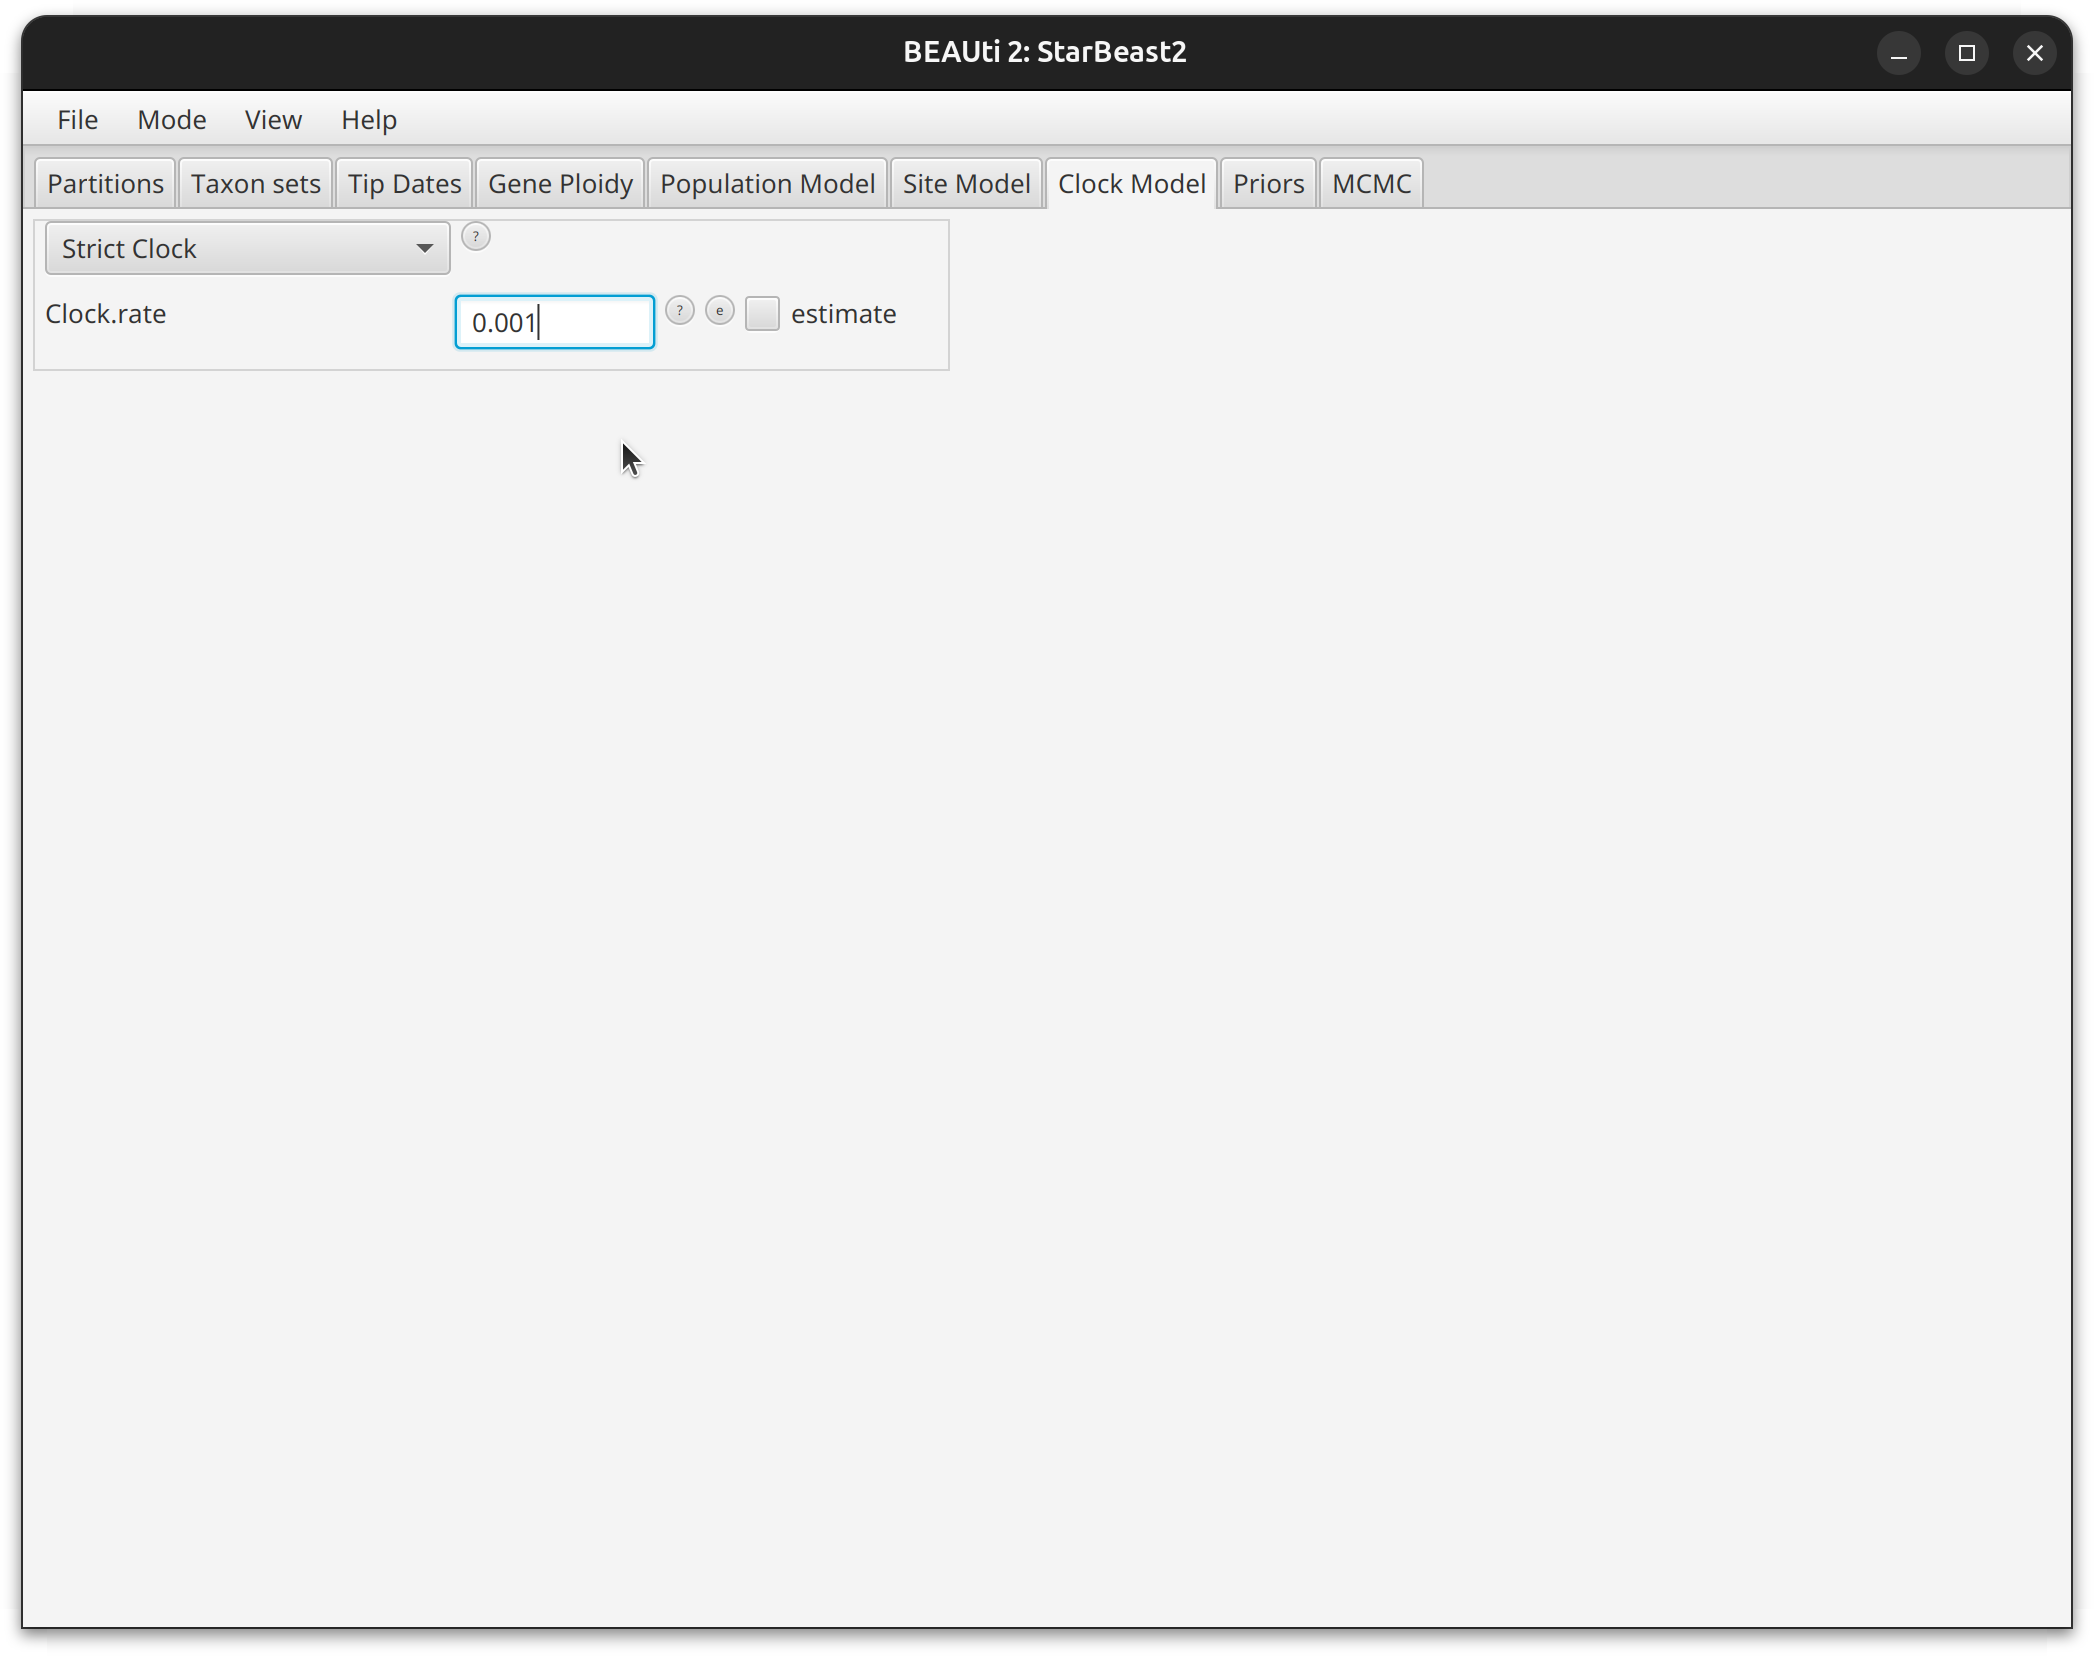
\includegraphics[width=0.8\textwidth]{figures/strictClockModel.png}
\caption
{Using an \textit{a priori} clock rate for calibration}
\label{fig:strictClockModel}
\end{figure}

You can also use the scientific notation shorthand, 1e-3, which is equivalent
to 0.001.

\subsection{Priors and MCMC}
\label{subsec:MCMC}

Open the Priors panel and change ``Yule Model'' to ``Birth Death Model''.
These models are identical, except the birth-death model allows for a
non-zero rate of extinction.

StarBEAST2 is an MCMC method. These kind of methods do better at estimating
the posterior distributions (of trees or other parameters) the longer they
are run, although after a point there are diminishing returns. The default
chain length in StarBEAST2 is 10 million states, but for this analysis we
need a bit more for good estimates; change the chain length to 40 million
(Figure~\ref{fig:chainLength})

\begin{figure}[htb!]
\centering
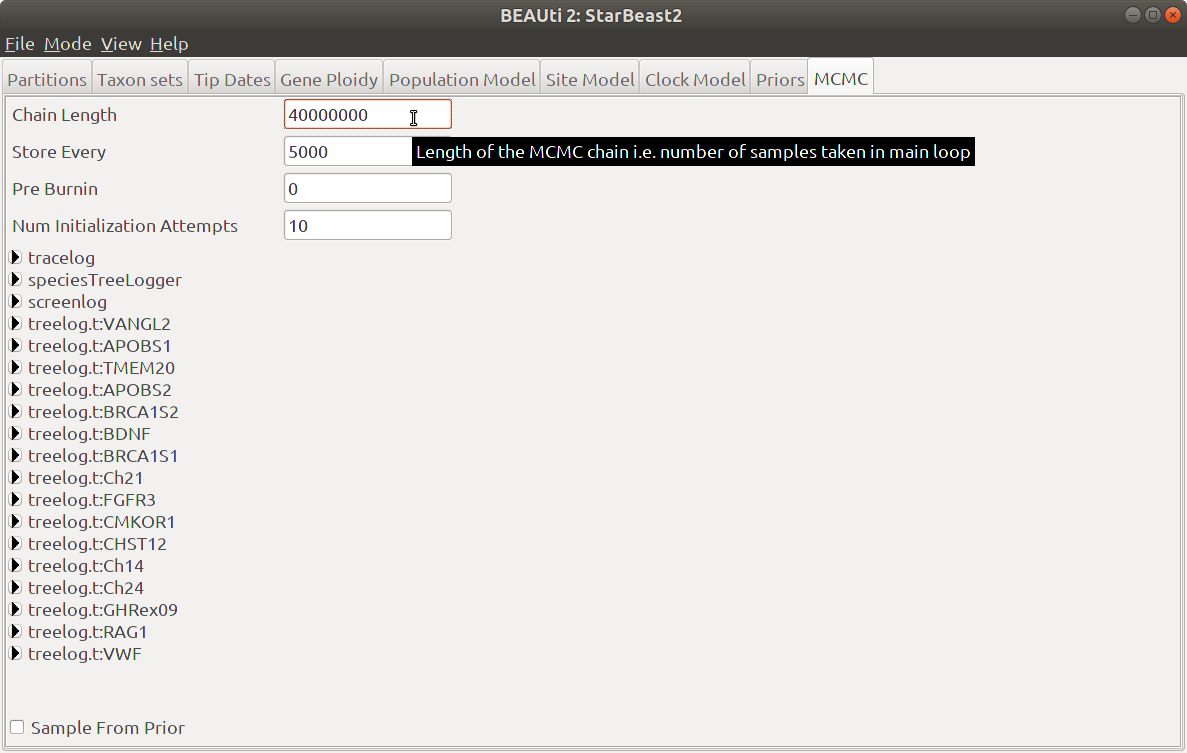
\includegraphics[width=0.8\textwidth]{figures/chainLength.png}
\caption
{Setting a longer MCMC chain length}
\label{fig:chainLength}
\end{figure}

\newpage{}

Save your model as an XML file -- in the folder you created before importing
alignments -- by clicking Save As in the File menu. Navigate to the folder
and give your XML file a name like ``CanisPhylogeny.xml''.

\subsection{Running BEAST}
\label{subsec:runningBEAST}

You can run BEAST from the command line or using the GUI. To run your XML
from the command line, first navigate to the folder you saved the XML file into.
Then run ``/path/to/beast/bin/beast CanisPhylogeny.xml''. Make sure to change
/path/to/beast to match the folder where BEAST is installed on your computer.

BEAST should take about 10 to 15 minutes to finish the chain. Sampled statistics
and various parameters will be saved to ``starbeast.log'', species trees to
``species.trees'', and separate gene tree files will be created for each locus. The command line
output should start off looking something like what follows:


\begin{verbatim}Checking out /home/huey/.beast/2.4/BEAST/lib
Loaded URL file:/home/huey/.beast/2.4/BEAST/lib/beast.jar
jardir = /home/huey/beast/lib/launcher.jar
Loading package BEAST v2.4.7
Loading package MM v1.0.5
Loading package SA v1.1.7
Loading package BEAST v2.4.7
Loading package starbeast2 v0.14.0
Loading package BEASTLabs v1.7.1

                   BEAST v2.4.7 Prerelease, 2002-2017
             Bayesian Evolutionary Analysis Sampling Trees
                       Designed and developed by
 Remco Bouckaert, Alexei J. Drummond, Andrew Rambaut & Marc A. Suchard
                                    
                     Department of Computer Science
                         University of Auckland
                        remco@cs.auckland.ac.nz
                        alexei@cs.auckland.ac.nz
                                    
                   Institute of Evolutionary Biology
                        University of Edinburgh
                           a.rambaut@ed.ac.uk
                                    
                    David Geffen School of Medicine
                 University of California, Los Angeles
                           msuchard@ucla.edu
                                    
                      Downloads, Help & Resources:
                           http://beast2.org/
                                    
  Source code distributed under the GNU Lesser General Public License:
                   http://github.com/CompEvol/beast2
                                    
                           BEAST developers:
   Alex Alekseyenko, Trevor Bedford, Erik Bloomquist, Joseph Heled, 
 Sebastian Hoehna, Denise Kuehnert, Philippe Lemey, Wai Lok Sibon Li, 
Gerton Lunter, Sidney Markowitz, Vladimir Minin, Michael Defoin Platel, 
                 Oliver Pybus, Chieh-Hsi Wu, Walter Xie
                                    
                               Thanks to:
          Roald Forsberg, Beth Shapiro and Korbinian Strimmer

Random number seed: 1512645447217

File: CanisPhylogeny.xml seed: 1512645447217 threads: 1\end{verbatim}

It will end with a bunch of statistics describing the performance of the MCMC operators:

\begin{verbatim}Operator                                                                Tuning    #accept    #reject      Pr(m)  Pr(acc|m)
UpDownOperator(clockUpDownOperator.c:BRCA1S1)                           0.8522      18169      50825     0.0019     0.2633 
ScaleOperator(TreeScaler.t:BRCA1S1)                                     0.8682      19465      49496     0.0019     0.2823 
ScaleOperator(TreeRootScaler.t:BRCA1S1)                                 0.4248      14918      54203     0.0019     0.2158 
Uniform(UniformOperator.t:BRCA1S1)                                           -     146565     198613     0.0094     0.4246 
SubtreeSlide(SubtreeSlide.t:BRCA1S1)                                    0.7795     120013     225596     0.0094     0.3473 
Exchange(Narrow.t:BRCA1S1)                                                   -     109470     235681     0.0094     0.3172 
Exchange(Wide.t:BRCA1S1)                                                     -       8117     336186     0.0094     0.0236 
WilsonBalding(WilsonBalding.t:BRCA1S1)                                       -      10344     335125     0.0094     0.0299 
[...]
DeltaExchangeOperator(FixMeanMutationRatesOperator)                     2.0294      88056     648890     0.0201     0.1195 
ScaleOperator(KappaScaler.s:APOBS1)                                     0.1987       7059      15949     0.0006     0.3068 
ScaleOperator(KappaScaler.s:APOBS2)                                     0.2034       7243      15463     0.0006     0.3190 
ScaleOperator(KappaScaler.s:BDNF)                                       0.1660       6783      16531     0.0006     0.2909 
ScaleOperator(KappaScaler.s:BRCA1S1)                                    0.1857       6903      15965     0.0006     0.3019 
ScaleOperator(KappaScaler.s:BRCA1S2)                                    0.1976       6794      16280     0.0006     0.2944 
ScaleOperator(KappaScaler.s:CHST12)                                     0.1751       6930      16559     0.0006     0.2950 
ScaleOperator(KappaScaler.s:CMKOR1)                                     0.1976       7162      15697     0.0006     0.3133 
ScaleOperator(KappaScaler.s:Ch14)                                       0.2973       6333      16470     0.0006     0.2777 
ScaleOperator(KappaScaler.s:Ch21)                                       0.2553       7159      15909     0.0006     0.3103 
ScaleOperator(KappaScaler.s:Ch24)                                       0.2272       6810      16334     0.0006     0.2942 
ScaleOperator(KappaScaler.s:FGFR3)                                      0.2009       7028      15842     0.0006     0.3073 
ScaleOperator(KappaScaler.s:GHRex09)                                    0.1926       7244      15595     0.0006     0.3172 
ScaleOperator(KappaScaler.s:RAG1)                                       0.2242       7336      15792     0.0006     0.3172 
ScaleOperator(KappaScaler.s:TMEM20)                                     0.2046       7077      15773     0.0006     0.3097 
ScaleOperator(KappaScaler.s:VANGL2)                                     0.1901       6838      15992     0.0006     0.2995 
ScaleOperator(KappaScaler.s:VWF)                                        0.2174       7618      15565     0.0006     0.3286 
starbeast2.NodeReheight2(Reheight.t:Species)                                 -     190932    2793110     0.0471     0.0640 
starbeast2.CoordinatedUniform(coordinatedUniform.t:Species)                  -     277295     318958     0.0094     0.4651 
starbeast2.CoordinatedExponential(coordinatedExponential.t:Species)     0.0724     357000     240475     0.0094     0.5975 
UpDownOperator(updownAll:Species)                                       0.6391      50943     186734     0.0038     0.2143 
starbeast2.RealCycle(constPopSizesSwap.Species)                         2.0000      23521      95986     0.0019     0.1968 k = 2
ScaleOperator(constPopSizesScale.Species)                               0.2694      28048      91487     0.0019     0.2346 
ScaleOperator(constPopMeanScale.Species)                                0.4184      11724      27838     0.0006     0.2963 
ScaleOperator(netDiversificationRateScale.t:Species)                    0.2074      10390      29138     0.0006     0.2629 
ScaleOperator(ExtinctionFractionScale.t:Species)                        0.1502       5748      14261     0.0003     0.2873 
UniformOperator(ExtinctionFractionUniform.t:Species)                         -      10374       9609     0.0003     0.5191 
SubtreeSlide(bdSubtreeSlide.t:Species)                                  0.0697     177124     419681     0.0094     0.2968 
WilsonBalding(bdWilsonBalding.t:Species)                                     -        371     597396     0.0094     0.0006 
Exchange(bdWide.t:Species)                                                   -       3255     594405     0.0094     0.0054 
Exchange(bdNarrow.t:Species)                                                 -      29181     567726     0.0094     0.0489 
Uniform(bdUniformOperator.t:Species)                                         -      45371     551315     0.0094     0.0760 
ScaleOperator(bdTreeRootScaler.t:Species)                               0.9259       9555     109831     0.0019     0.0800
ScaleOperator(bdTreeScaler.t:Species)                                   0.9876      21203      98760     0.0019     0.1767 

     Tuning: The value of the operator's tuning parameter, or '-' if the operator can't be optimized.
    #accept: The total number of times a proposal by this operator has been accepted.
    #reject: The total number of times a proposal by this operator has been rejected.
      Pr(m): The probability this operator is chosen in a step of the MCMC (i.e. the normalized weight).
  Pr(acc|m): The acceptance probability (#accept as a fraction of the total proposals for this operator).


Total calculation time: 756.696 seconds
End likelihood: -16953.439185360676\end{verbatim}


\subsection{Checking the log file}
\label{subsec:checkLog}

To check parameters other than species tree topologies and branch values, or to verify
that the chain has been run long enough to reliably represent the posterior distribution,
we will use Tracer. Start the Tracer app and then open the ``starbeast.log'' file.
The first statistic that will be displayed is a histogram of the log posterior probability
(Figure~\ref{fig:tracerPosterior}).

\begin{figure}[htb!]
\centering
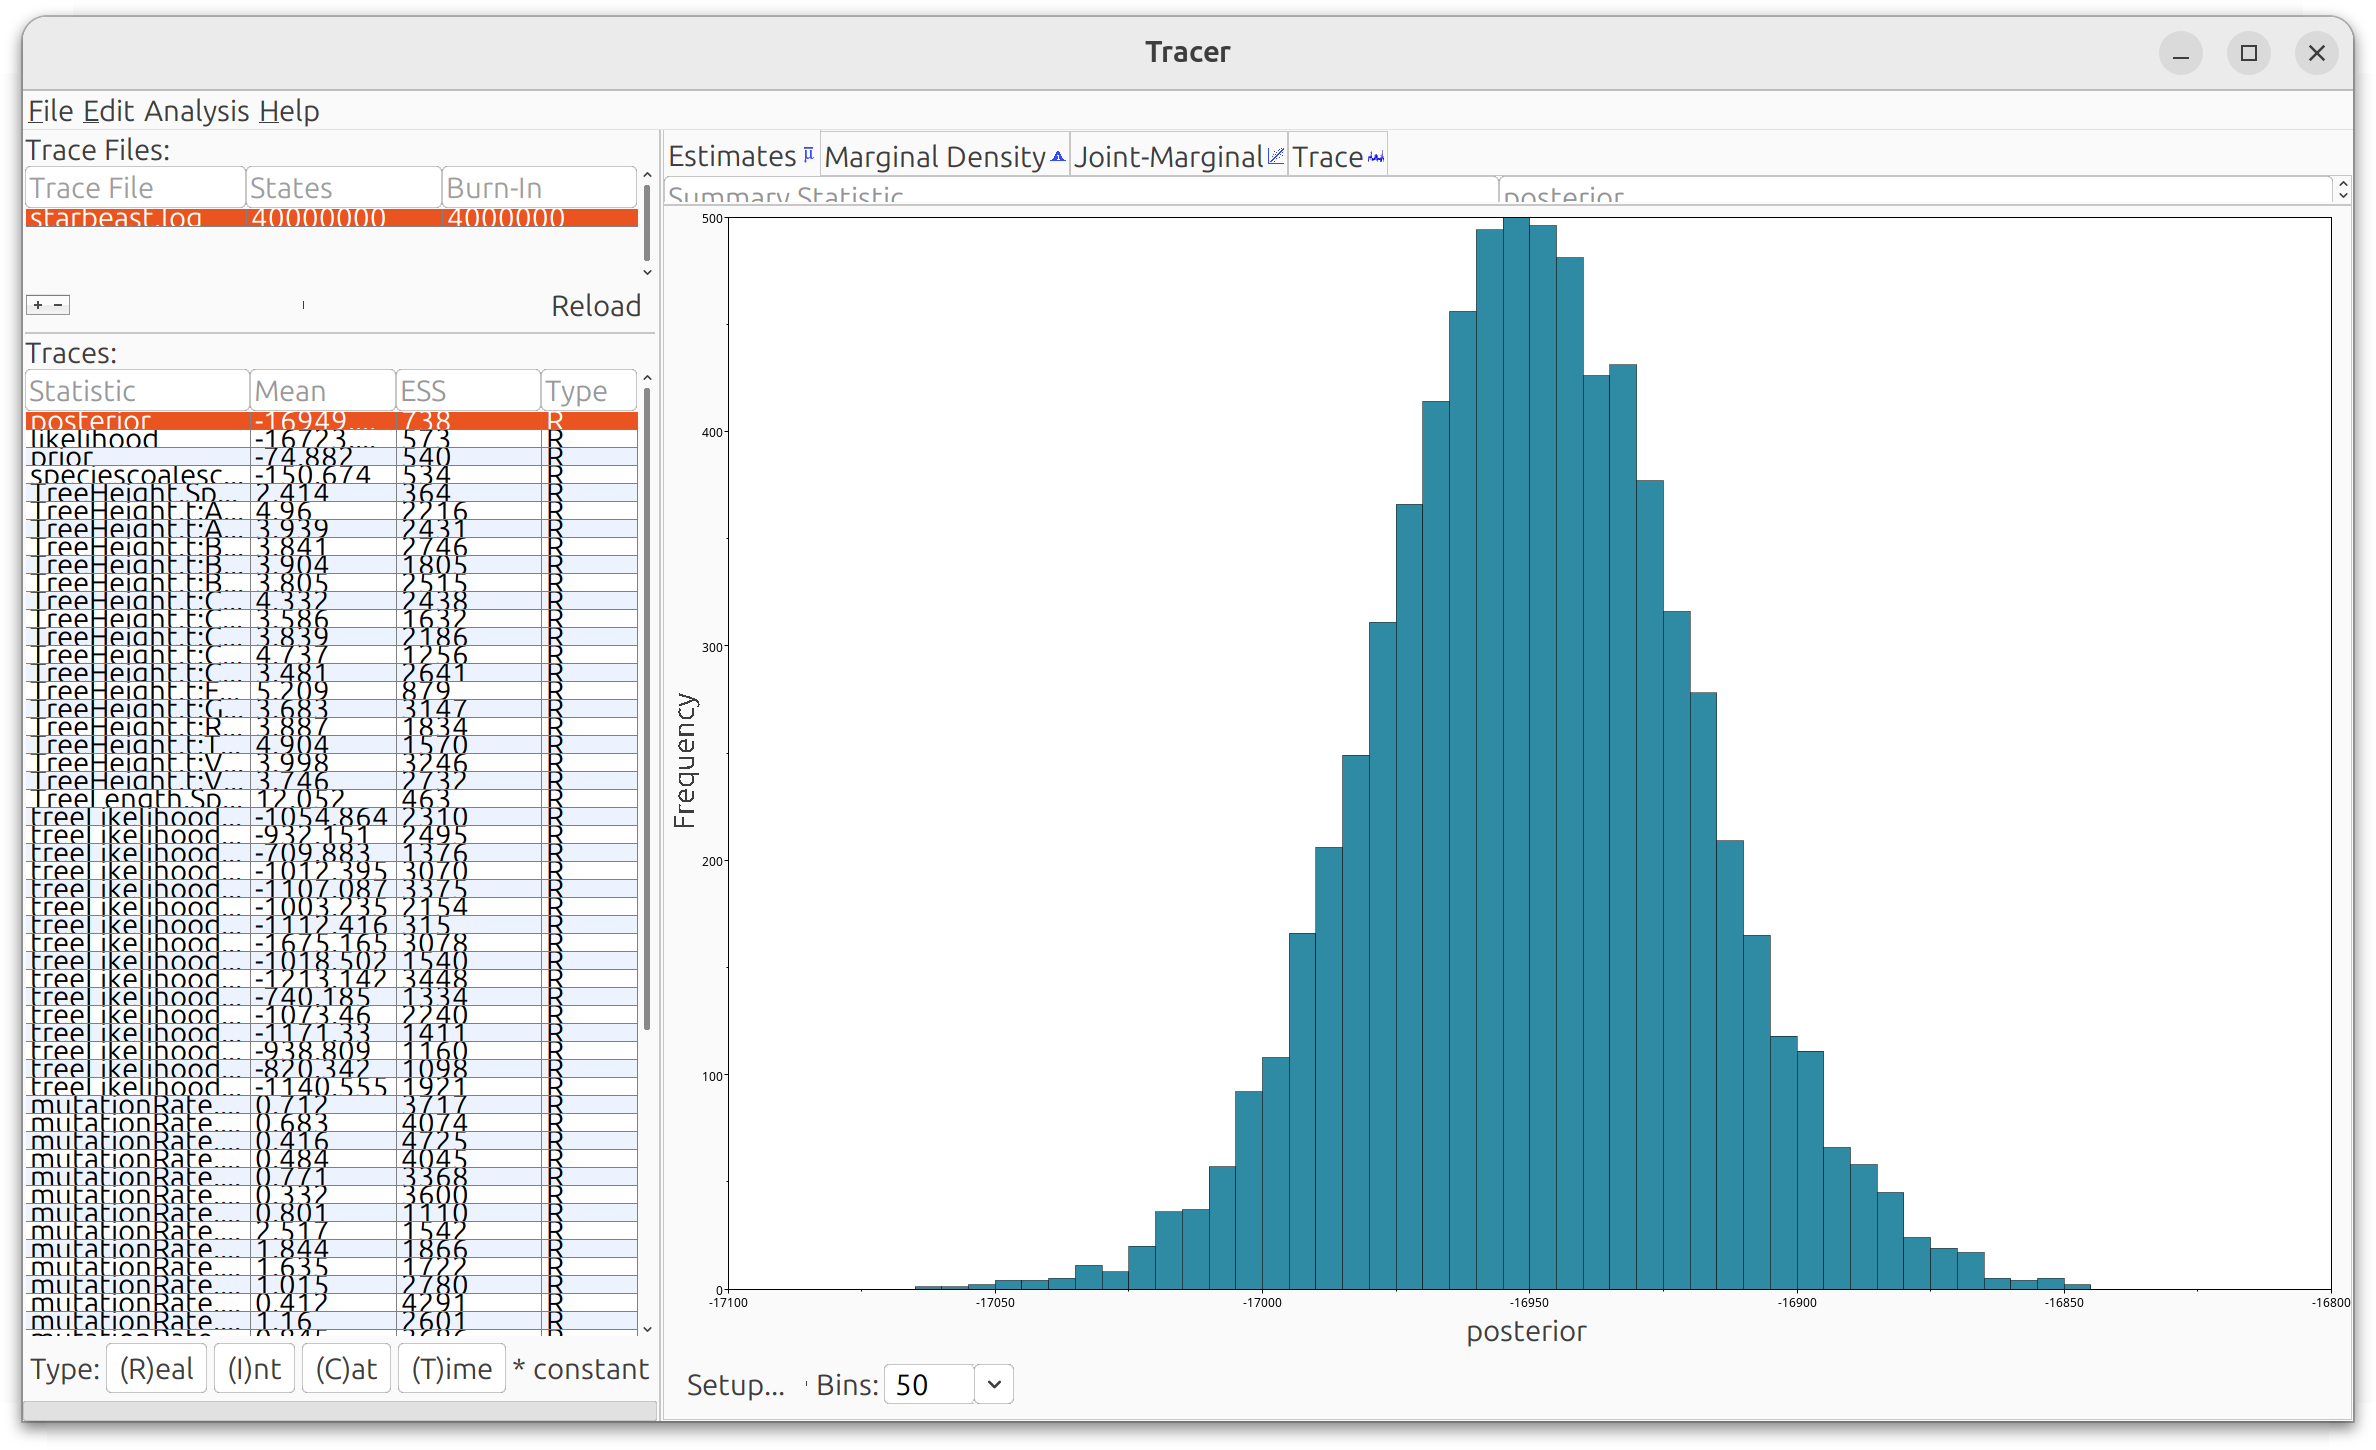
\includegraphics[width=0.8\textwidth]{figures/tracerPosterior.png}
\caption
{Opening a log file in Tracer}
\label{fig:tracerPosterior}
\end{figure}

The posterior probability is the sum of the likelihood (which is the sum of
log phylogenetic likelihoods for all sites for all loci), the prior
probability (which is the sum of log prior probabilities for all parameters),
and the speciescoalescent (which is the sum of log coalescent probabilities for
all gene trees). TreeHeight.Species is the height of the root node of the
species tree, and TreeLength.Species is the sum of all branch lengths in the
species tree.

Tracer computes effective sample sizes (ESS) for each logged statistic and
parameter. As a rule, ESS values should be at least 200, particularly for
the important statistics just noted and for parameters of interest. Because of the stochastic
nature of MCMC algorithms, your values \textbf{will be different} to those in
Figure~\ref{fig:tracerPosterior}.

\subsection{Checking the species trees}
\label{subsec:checkTrees}

Start the DensiTree app (included with BEAST2), and then open the
``species.trees'' file. Under the Show panel, enable the Root Canal tree to
get an idea of the most plausible species tree. Then open the Grid panel, and
enable the full grid (Figure~\ref{fig:densitree}). If you want to check the
clade posterior probabilities, select ``View clade toolbar'' from the Window menu.

\begin{figure}[htb!]
\centering
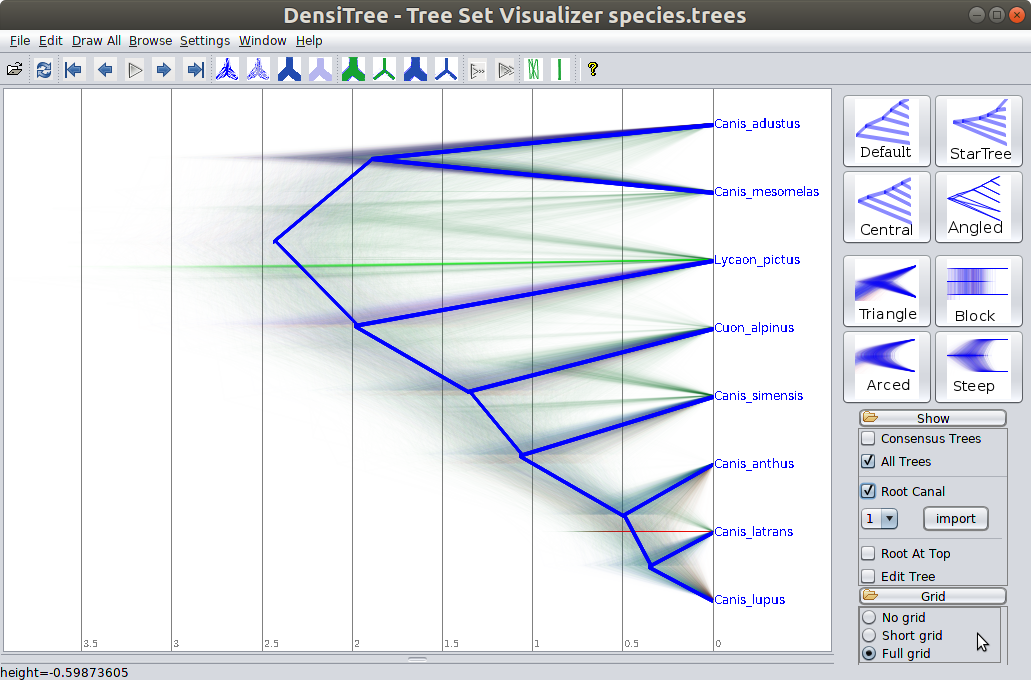
\includegraphics[width=0.8\textwidth]{figures/densitree.png}
\caption
{Viewing the species trees in DensiTree}
\label{fig:densitree}
\end{figure}

You can see that using a fixed clock rate of $10^{-3}$ substitutions per site
per year, the split between \textit{Canis latrans} (coyotes) and \textit{Canis lupus}
(wolves) is probably less than 500,000 years ago. The age of the most
recent common ancestor (MRCA) of extant \textit{Canis} taxa is approximately 2.5 million
years ago, more recent than the split between humans and chimpanzees \parencite{PradoMartinez2013}.

\subsection{Generating a summary tree}
\label{subsec:makeSummaryTree}

Summary trees are a way of reducing a posterior distribution of tree
topologies and times to a single tree. This is often more readable than the
cloud of trees that DensiTree displays, but researchers should be cautious not
to give it too much emphasis because for most clades and data
sets there is substantial uncertainty in the posterior distribution of
topologies and times.

To generate a summary tree, open the Tree Annotator app included with BEAST2.
Set the burnin percentage to 10 and choose the ``species.trees'' file generated by
StarBEAST2 as the input file. Specify the output file to be something sensible
like ``summary.tree'' and click Run to generate the summary tree
(Figure~\ref{fig:treeAnnotator}).

\begin{figure}[htb!]
\centering
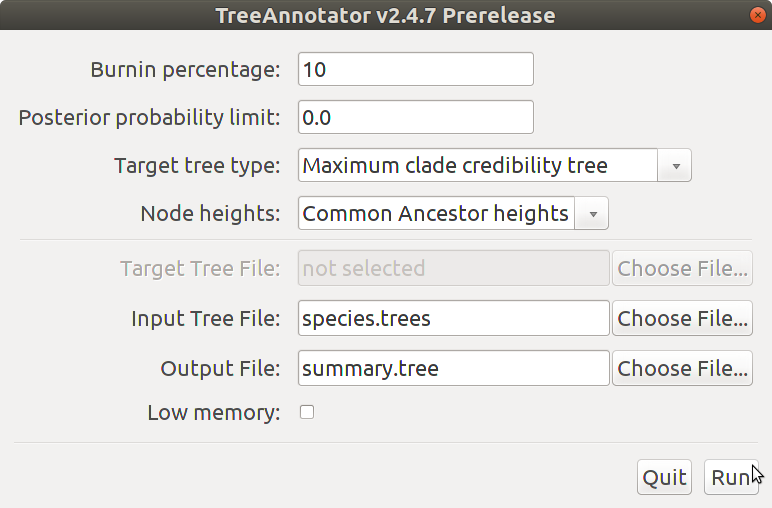
\includegraphics[width=0.5\textwidth]{figures/treeAnnotator.png}
\caption
{Running Tree Annotator}
\label{fig:treeAnnotator}
\end{figure}

\newpage{}

Now start FigTree and open the summary tree file. Enable Branch Labels,
and expand the Branch Labels panel. Choose ``dmv1\_95\%\_HPD'', and set
the number of significant digits to 2. Now the 95\% highest posterior
density (HPD) intervals of
effective population sizes will be displayed on each branch
(Figure~\ref{fig:figtree}).

\begin{figure}[htb!]
\centering
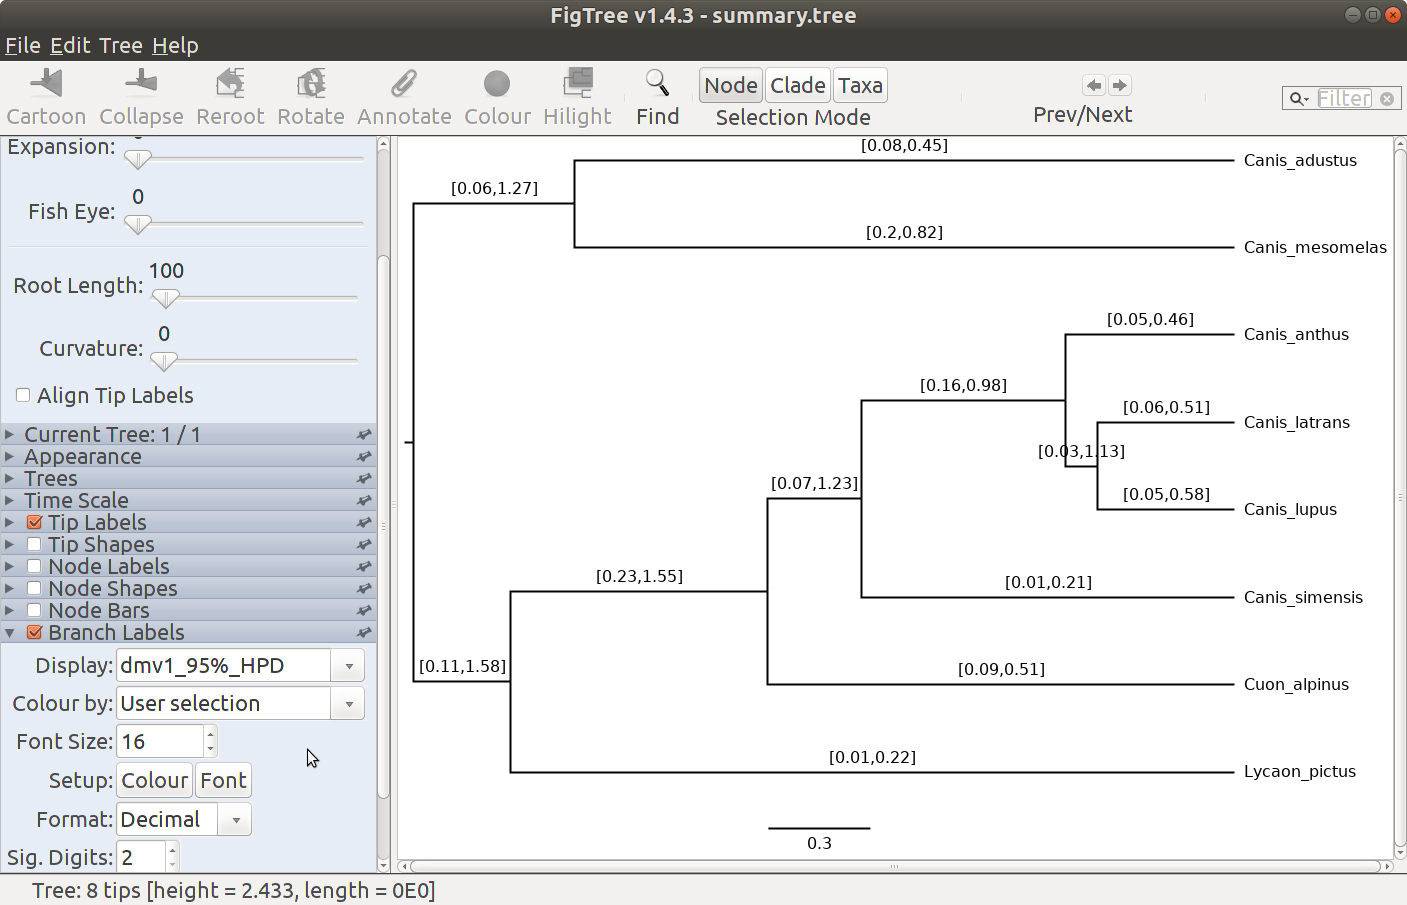
\includegraphics[width=0.8\textwidth]{figures/figtree.png}
\caption
{Running FigTree}
\label{fig:figtree}
\end{figure}

\newpage{}

In StarBEAST2 and many other BEAST packages, effective population sizes are
scaled by generation time. That means if generation times (the average
number of years from zygote to zygote) vary between species in your
analysis, the effective population sizes of different branches cannot be
directly compared.

If the average generation time is 5 years, and our tree is scaled in millions
of years, then the generation time is $5\times10^{-6}$. To get effective
population sizes in numbers of individuals, divide each value by the
generation time. So if the scaled effective population size is 1, that
will correspond to 200,000 individuals.

The effective population sizes inferred in this tutorial appear to have
roughly an order of magnitude of uncertainty, and more precise estimates would require
a more informative data set. This could be achieved by sampling more
individuals or more loci.

\clearpage{}

\section{Estimating per-species clock rates}
\label{sec:relaxedClock}

We can estimate molecular clock rates separately for each species using
a relaxed clock model, for example the uncorrelated log-normal (UCLN) model.
First create a new folder for this analysis with a sensible name, something
like ``CanisUCLN''. Relaunch BEAUti, and select ``SpeciesTreeUCLN'' from the
Templates submenu of the File menu (Figure~\ref{fig:speciesTreeUCLN}).

\begin{figure}[htb!]
\centering
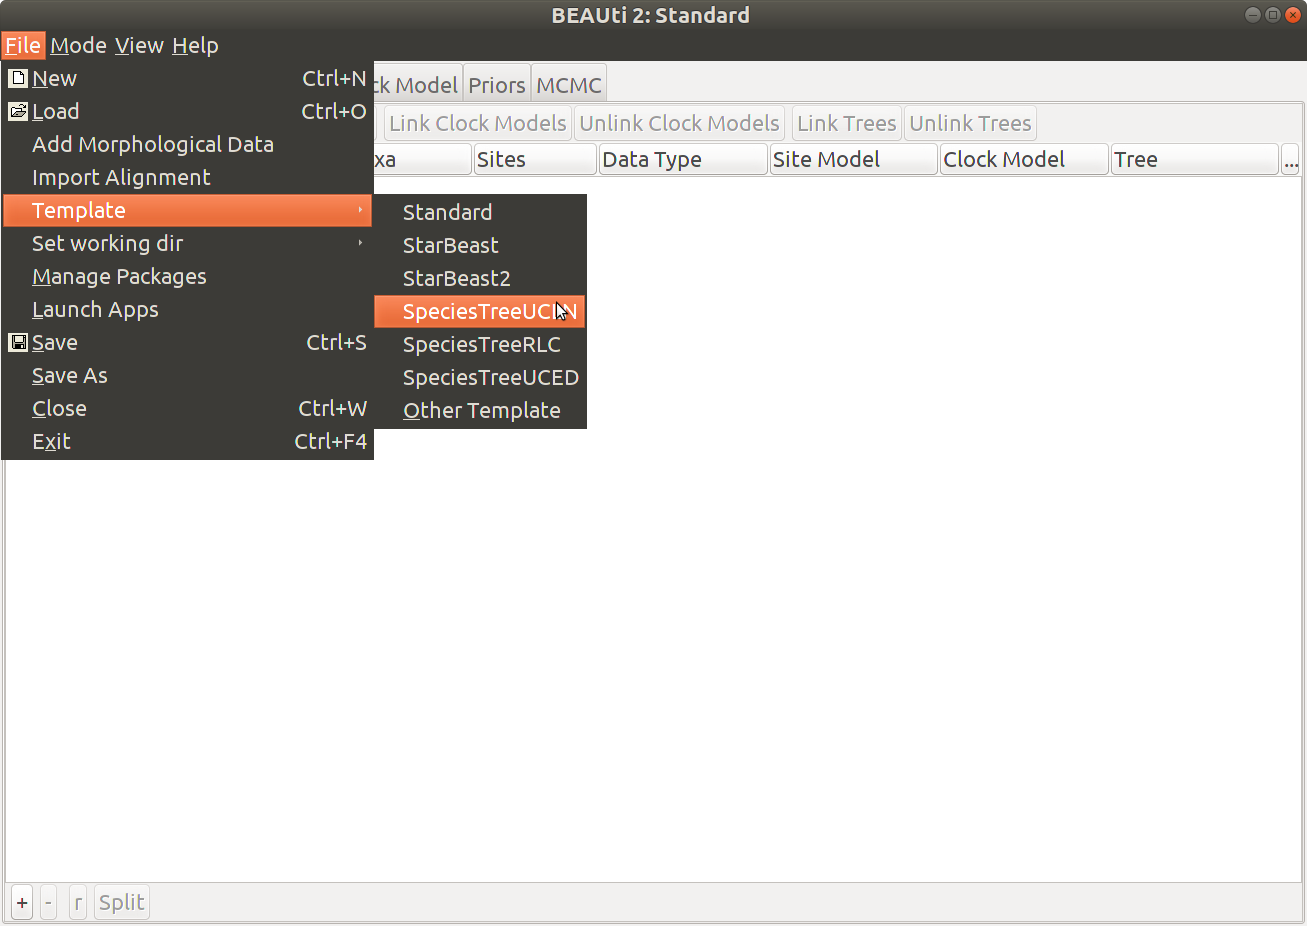
\includegraphics[width=0.8\textwidth]{figures/speciesTreeUCLN.png}
\caption
{Starting a UCLN relaxed clock analysis}
\label{fig:speciesTreeUCLN}
\end{figure}

Import the same FASTA files as in
subsection~\ref{subsec:importingAlignments}
(Figure~\ref{fig:fastaFileImport}). For any of the species tree relaxed clock
templates, do \textbf{NOT} link the clock models. This will break the inference
of per-species clock rates.

Assign the same species names as in
subsection~\ref{subsec:speciesNames} (Figure~\ref{fig:guessTaxonMap}, \ref{fig:taxonMap}). This time
we will keep the default setting for the population model (Analytical Integration), so that our analysis will run slightly faster. Set all
the site models to HKY with empirical frequencies as in
subsection~\ref{subsec:siteModel} (Figure~\ref{fig:hky}, \ref{fig:cloneSiteModel}).

Open the Clock Model tab, and manually set the Clock.rate to 0.001 (or
equivalently 1e-3) for \textbf{every} locus (Figure~\ref{fig:uclnClockRates}).
This is necessary because for technical reasons we cannot link the clock
models for the species tree relaxed clock templates.

\begin{figure}[htb!]
\centering
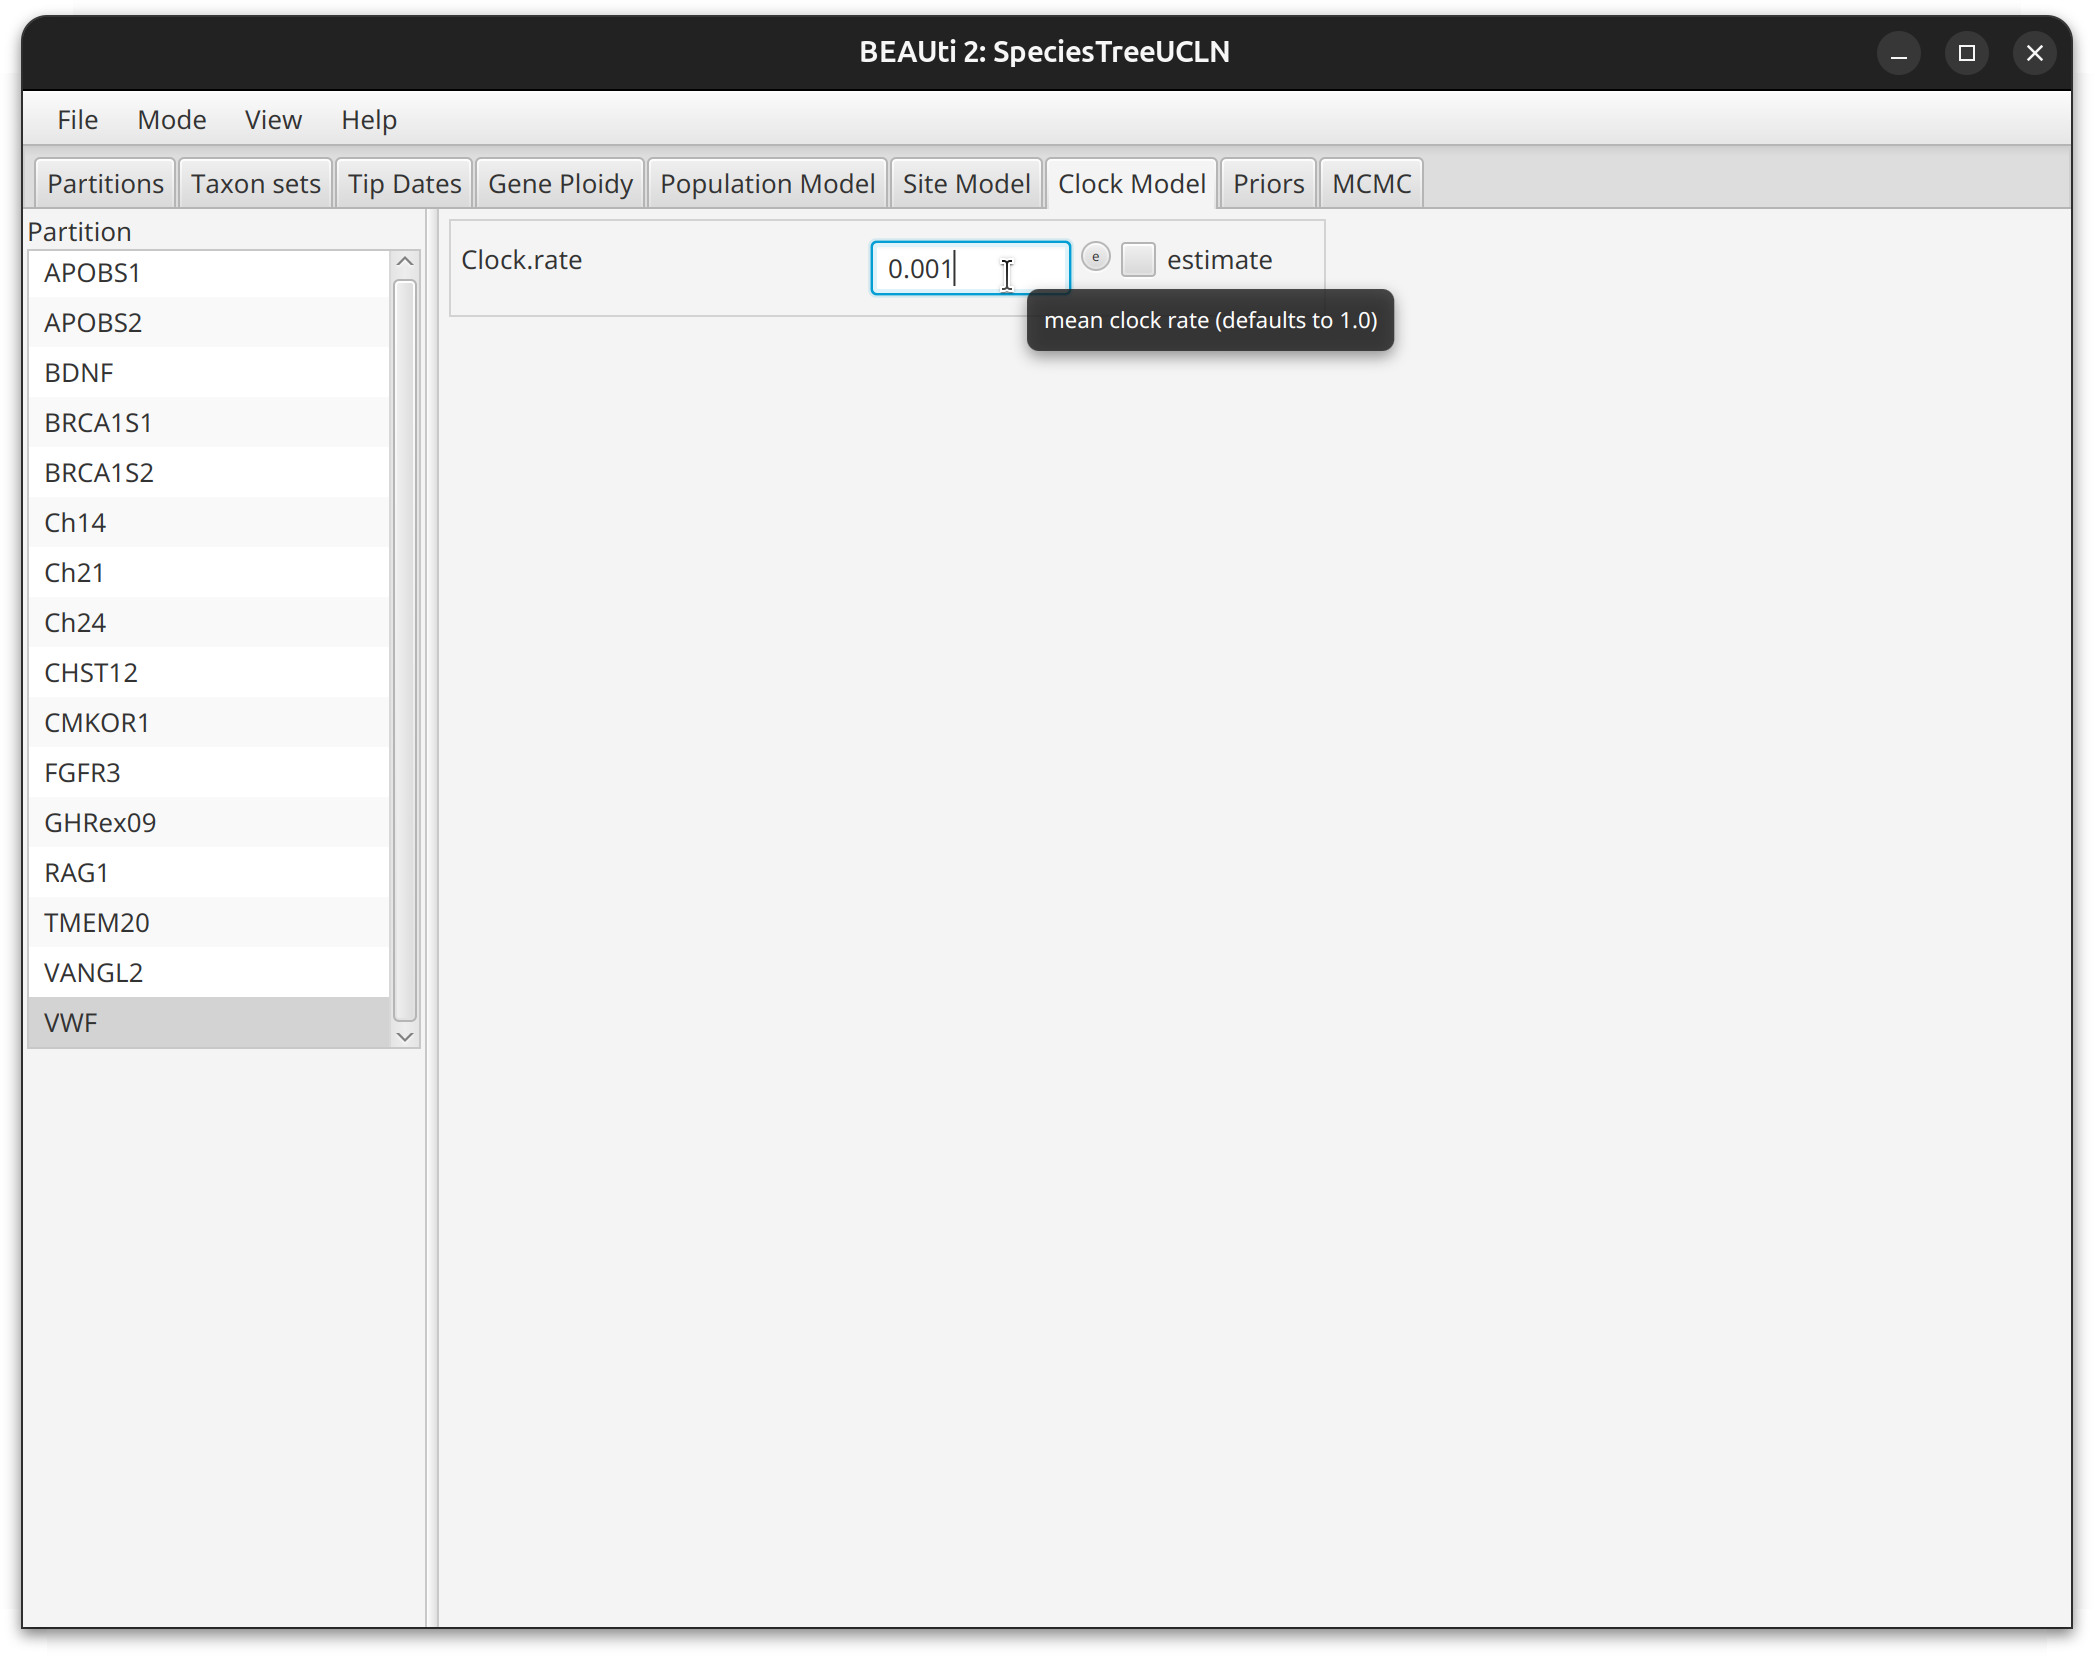
\includegraphics[width=0.8\textwidth]{figures/uclnClockRates.png}
\caption
{Manually setting every clock rate}
\label{fig:uclnClockRates}
\end{figure}

Open the Priors tab and change the species tree prior from Yule to Birth-Death
to allow for extinction. Finally, open the MCMC tab and change the length of
the chain to 40 million, as in subsection~\ref{subsec:MCMC}
(Figure~\ref{fig:chainLength}). Save the file in the folder you created
previously for this analysis, and give it a sensible name like ``CanisUCLN.xml''.

\newpage{}

Run the MCMC chain by opening the XML file in BEAST, or running it from
the command line as in subsection~\ref{subsec:runningBEAST}. This will
take about twice as long (20 to 30 minutes) as the fixed clock analysis,
because relaxed clocks are more computationally intensive.

After BEAST has finished, open the ``starbeast.log'' file in Tracer to
check that the important statistics have ESS values of at least 200.
Select the branchRatesStdev.Species parameter (Figure~\ref{fig:tracerUCLN}).

\begin{figure}[htb!]
\centering
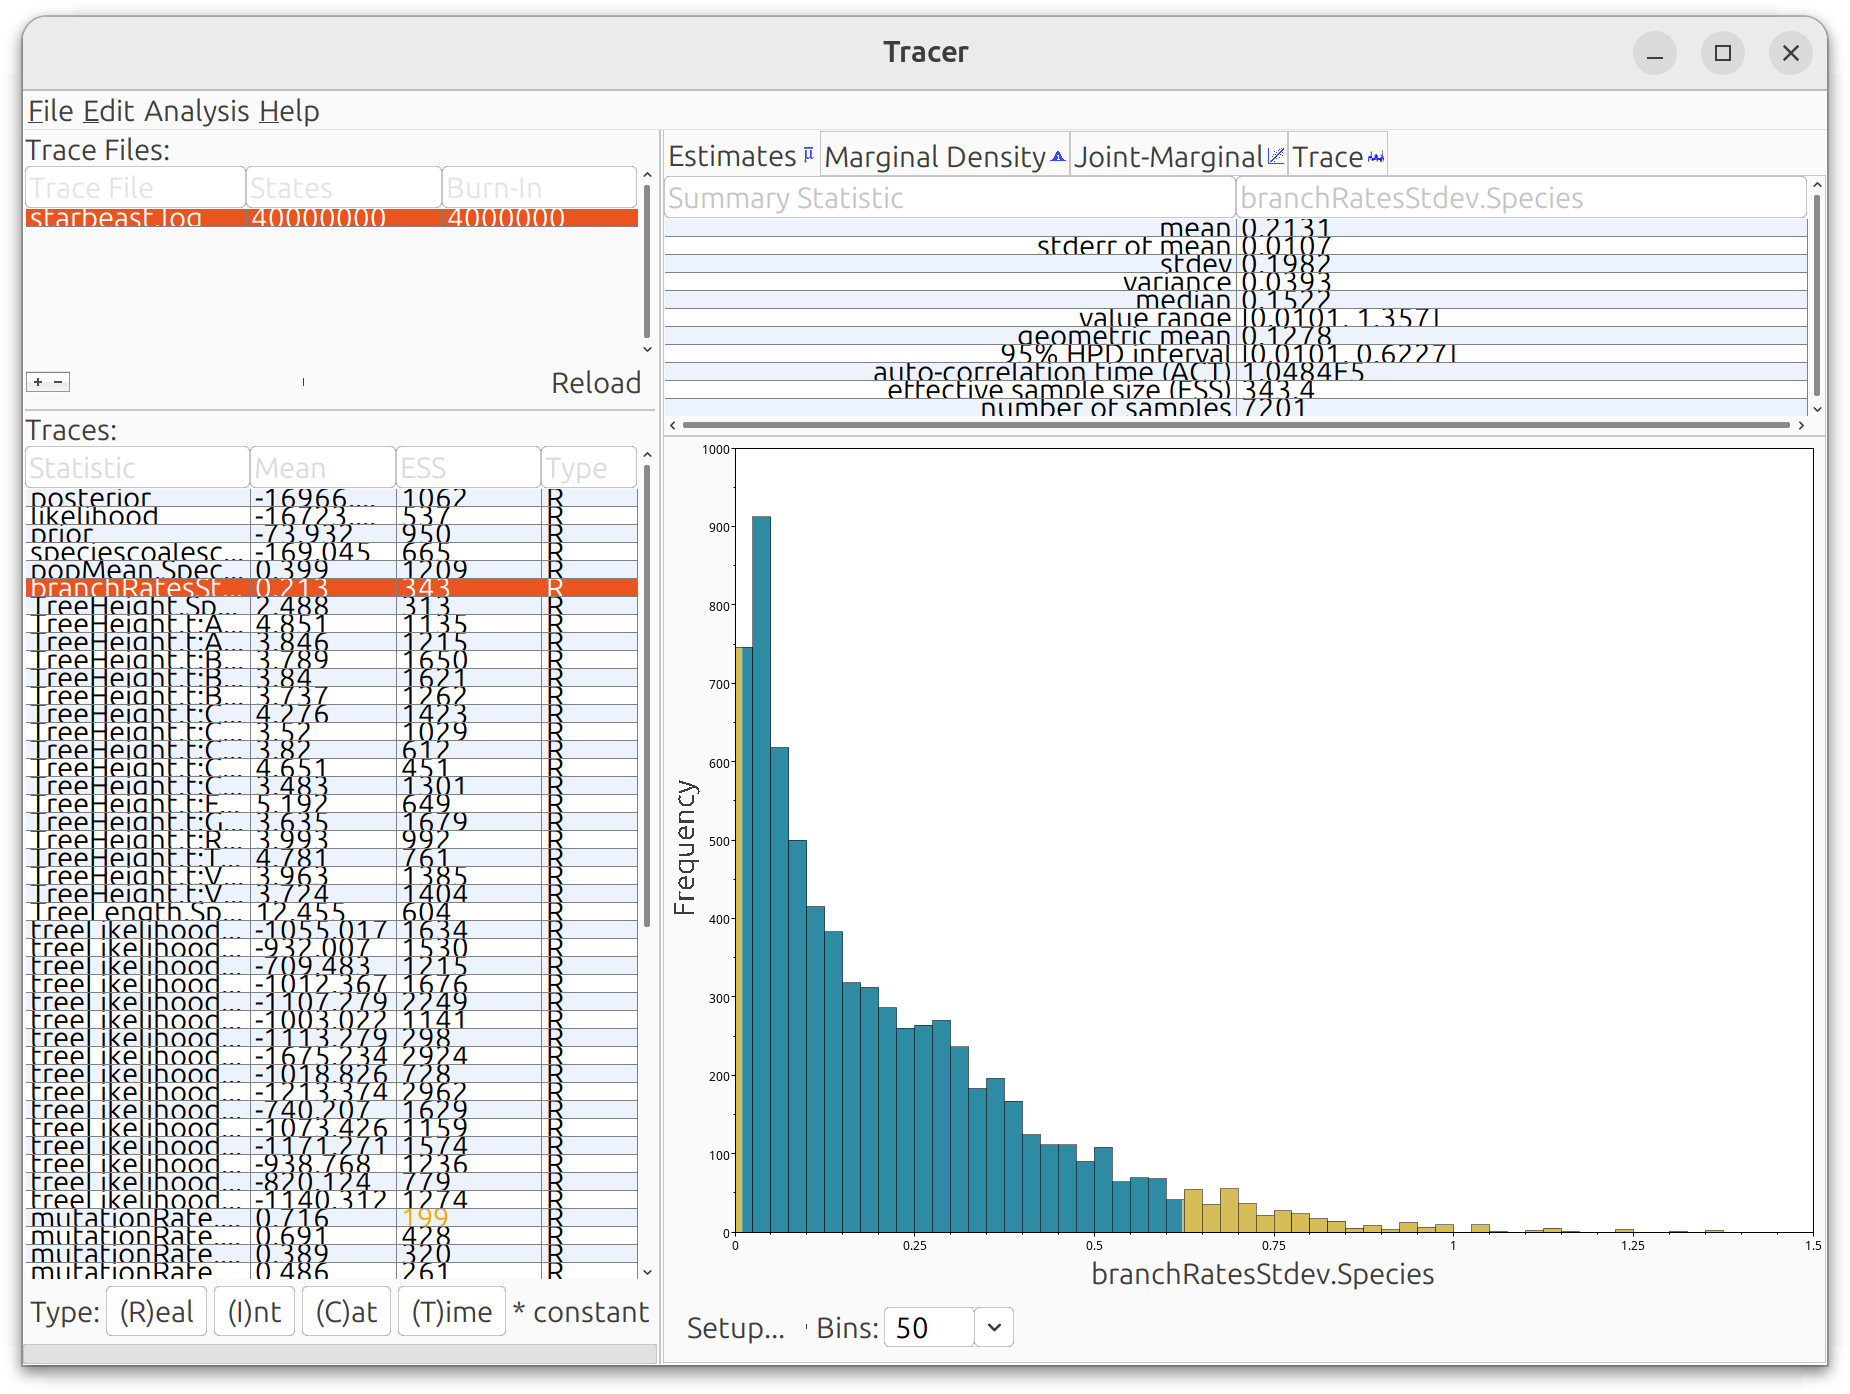
\includegraphics[width=0.8\textwidth]{figures/tracerUCLN.png}
\caption
{Checking the species tree relaxed clock analysis in Tracer}
\label{fig:tracerUCLN}
\end{figure}

This parameter models the spread of molecular clock rates among branches in
the species tree. The default prior for this parameter in StarBEAST2 is a
log-normal distribution with a mean of 1, but the posterior distribution of this
parameter has a mean of about 0.2. This means that the data is pulling this
parameter lower, probably because there is very little variation in clock
rates between species. Indeed the mode of the posterior distribution is about
zero, suggesting that a strict clock may be more appropriate
(Figure~\ref{fig:tracerUCLN}).

Now create a summary tree from the ``species.trees'' file using Tree
Annotator, as in subsection~\ref{subsec:makeSummaryTree}
(Figure~\ref{fig:treeAnnotator}). Again give it a sensible name like
``summary.tree''. Open up the summary tree file in FigTree. Enable Branch Labels,
and expand the Branch Labels panel. Choose ``rate\_95\%\_HPD'', and set
the number of significant digits to 2. Now the 95\% HPD intervals of
relative clock rates will be displayed on each branch
(Figure~\ref{fig:figtreeUCLN}).

\begin{figure}[htb!]
\centering
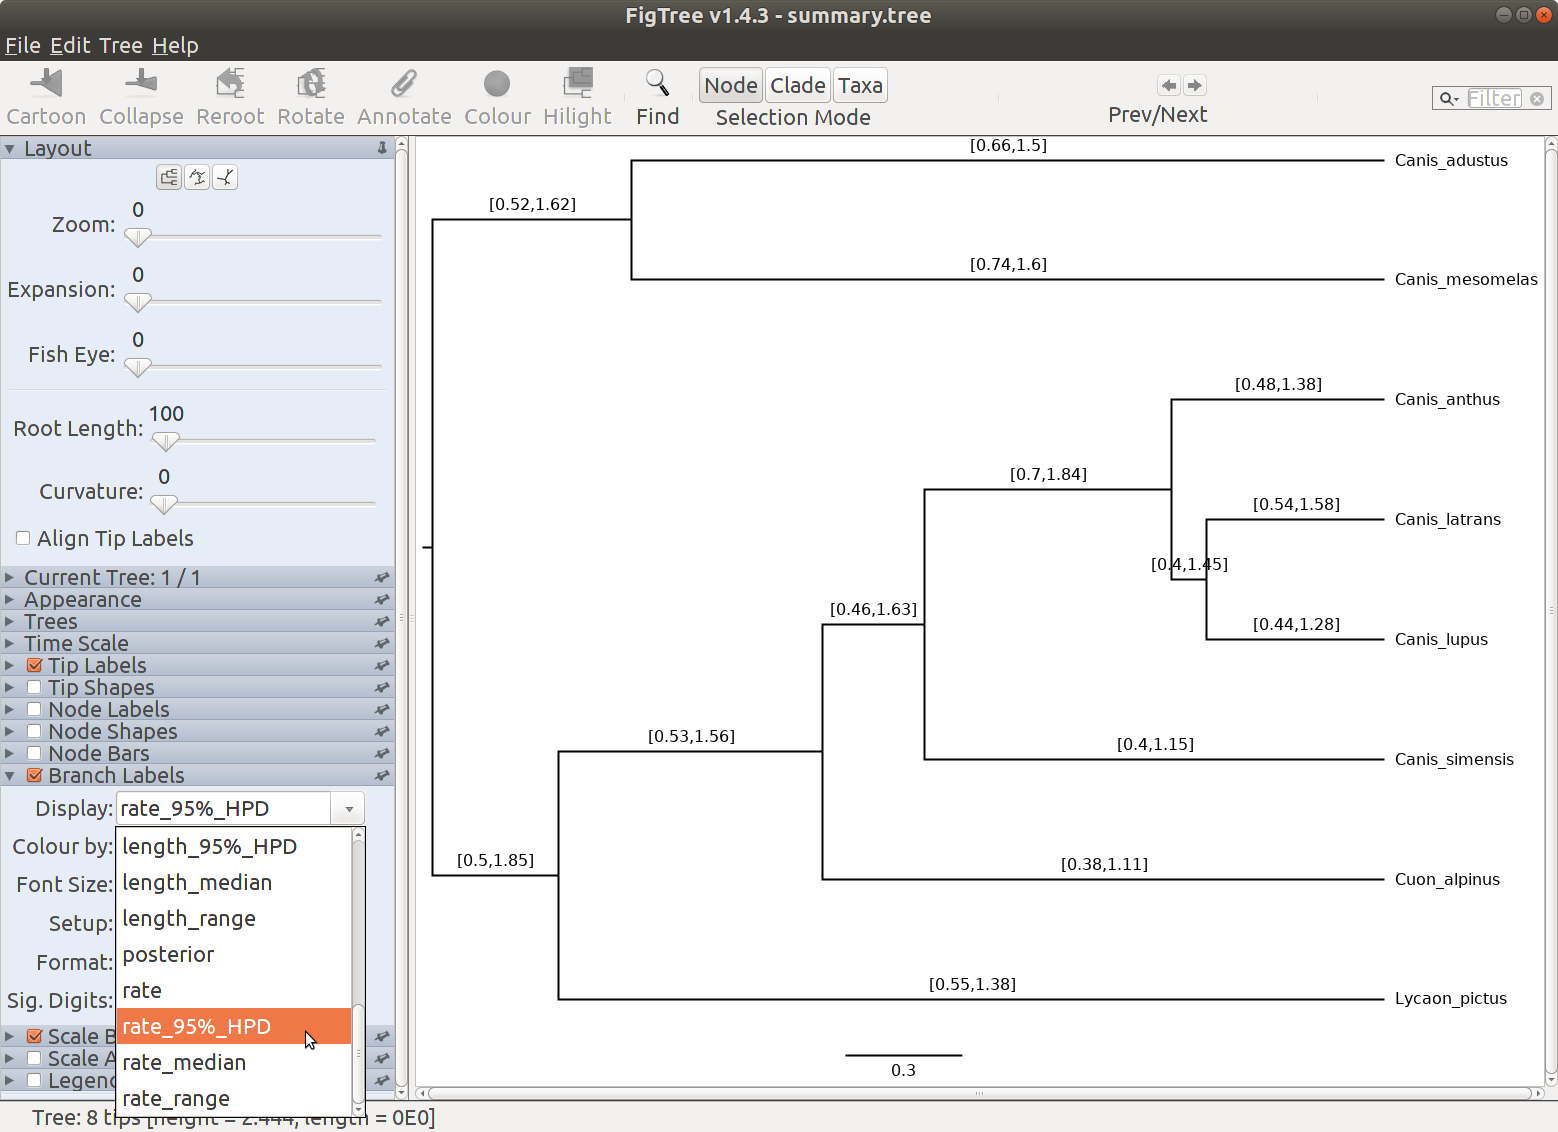
\includegraphics[width=0.8\textwidth]{figures/figtreeUCLN.png}
\caption
{Checking the species tree relaxed clock analysis in FigTree}
\label{fig:figtreeUCLN}
\end{figure}

All of the species tree branches have clock rate HPD intervals
that include 1, further suggesting that a strict clock may be more
appropriate for this clade. These rates are obviously relative, and
to get absolute rates in substitutions per site per million years,
they must be scaled by the \textit{a priori} clock rate of 0.001.

\clearpage{}

\section{Total evidence tip-dating}
\label{sec:FBD}

The versions of StarBEAST2 from 14 onwards include the ability to combine
tip-dating using the fossilized birth death (FBD) process with multispecies
coalescent (MSC) inference of species and gene trees. We call this integrative
model ``FBD-MSC''. To begin your analysis, creat a new folder for this
purpose with a sensible name, something like ``CanisFBD''.

\textbf{When setting up an FBD-MSC analysis in BEAUti, it is necessary to
import morphological data \ul{after} specifying the taxon sets \ul{and} the
tree model, but \ul{before} specifying the tip dates.} The following steps
will be consistent with that ordering. First, repeat
section~\ref{sec:speciesTree} from subsection~\ref{subsec:importingAlignments}
to and including \ref{subsec:speciesNames}. Leave the population model set at
the default (Analytical Integration) to save time, then set
all site models to HKY with empirical frequencies as in
subsection~\ref{subsec:siteModel}.

Before adding the morphological data, go to the Priors panel and change
the prior on the species tree from Yule to FBD
(Figure~\ref{fig:changeTreePrior}). This is necessary because the inclusion of
fossil taxa means our species tree will be \textit{serially sampled} rather
than \textit{ultrametric}. StarBEAST2 gives you the option of various
birth-death models -- Yule, Calibrated Yule, Birth Death and FBD -- but only
FBD is valid for serially sampled trees.

\begin{figure}[htb!]
\centering
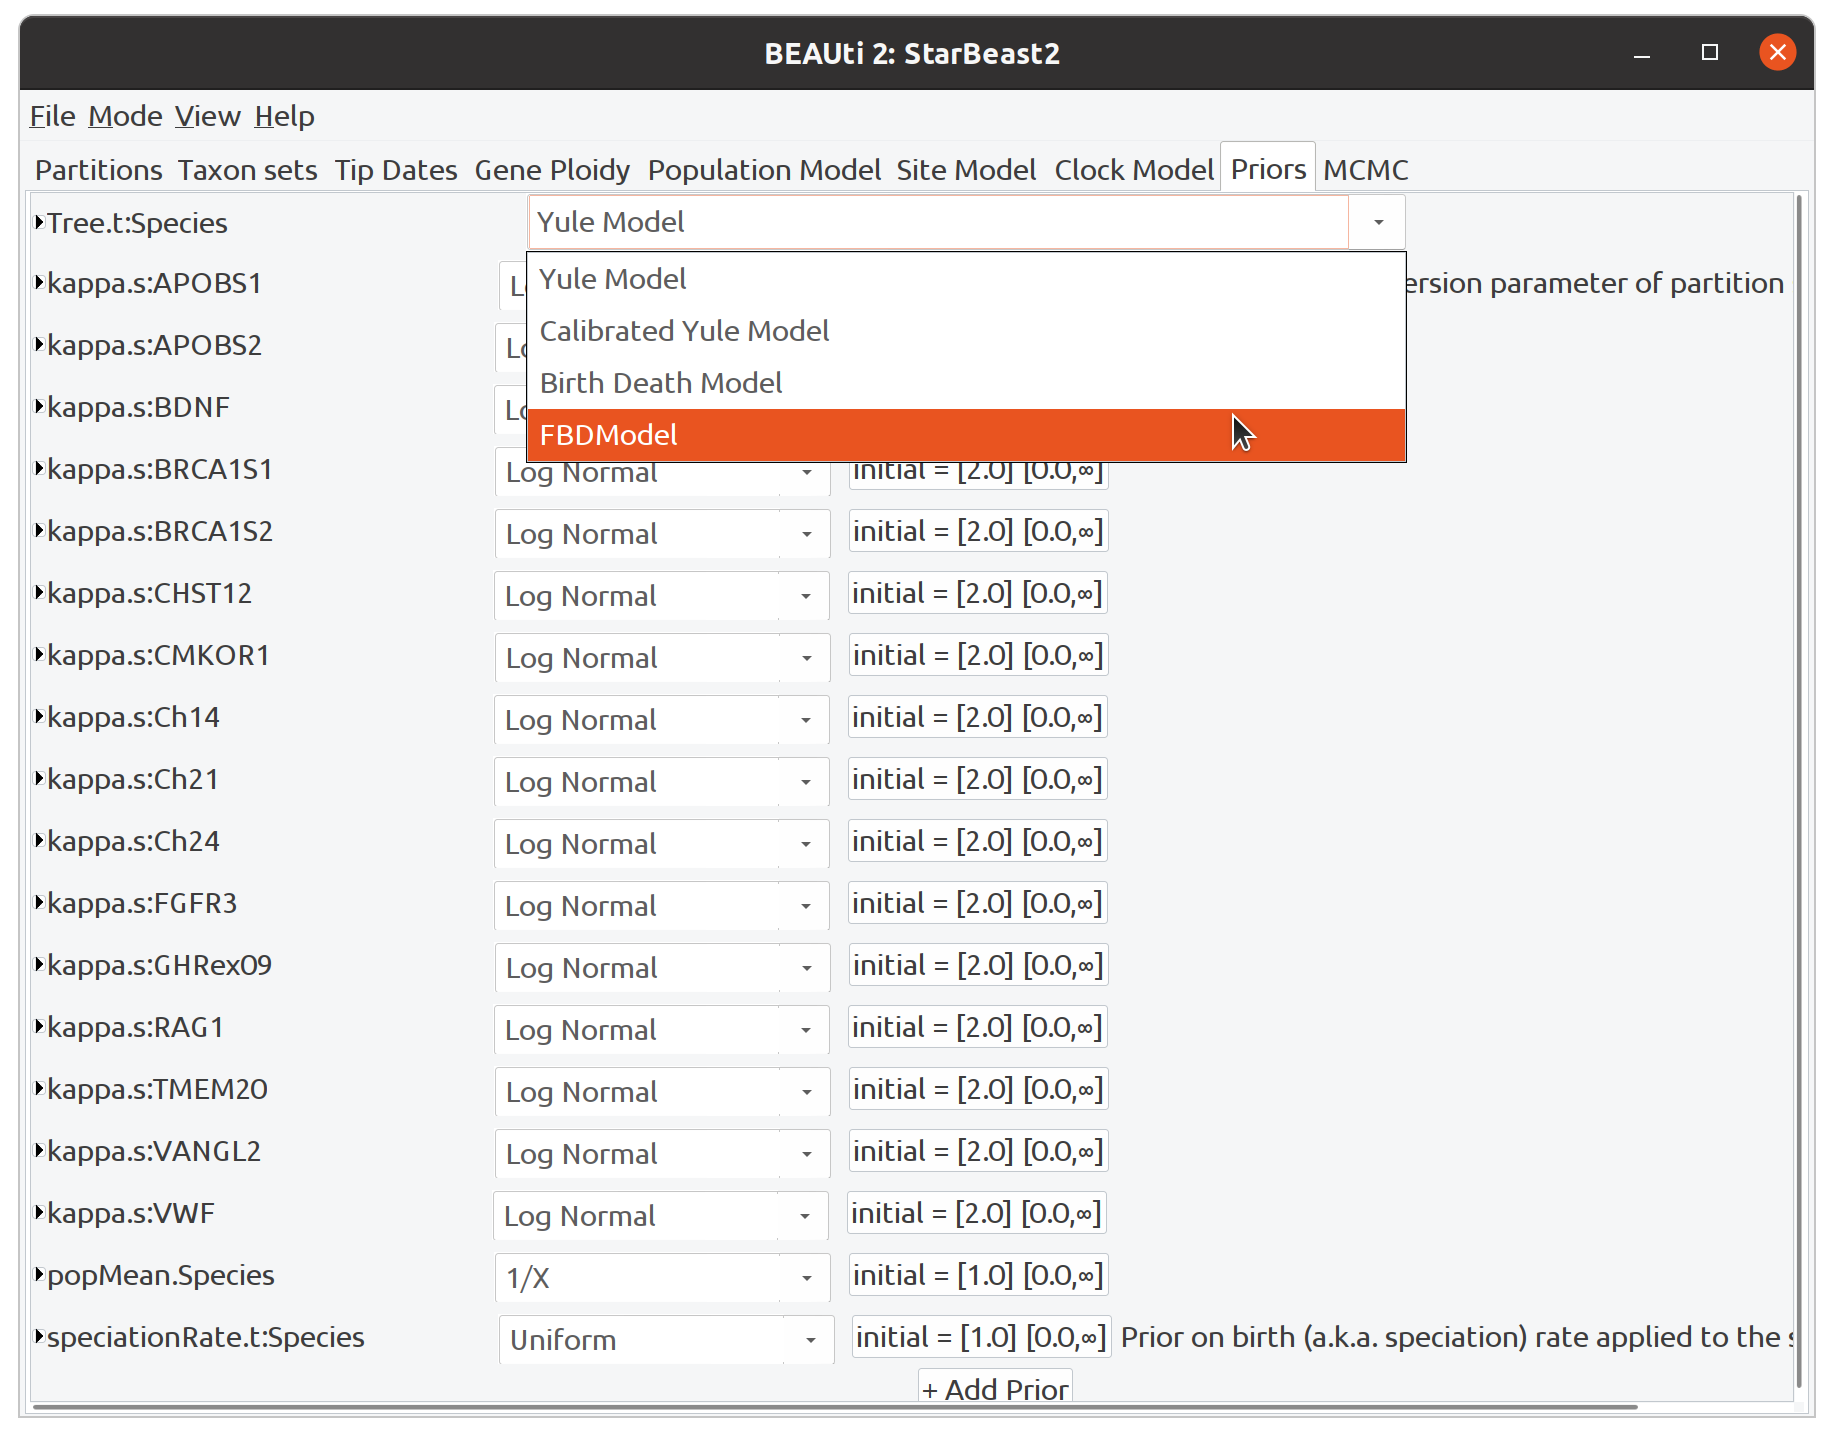
\includegraphics[width=0.8\textwidth]{figures/changeTreePrior.png}
\caption
{Change the tree model from Yule to FBD.}
\label{fig:changeTreePrior}
\end{figure}

\newpage{}

Now go back to the Partitions tab, and from the File menu select
``Add Morphology to Species Tree'' (Figure~\ref{fig:addMorphology}).
Navigate to the data folder of the tutorial and import the
``morphology\_canis.nex'' file.\footnote{This file contains recorded states for 50
morphological characters of \textit{Canis} species and some related species,
taken from \cite{Slater2015}.}

\begin{figure}[htb!]
\centering
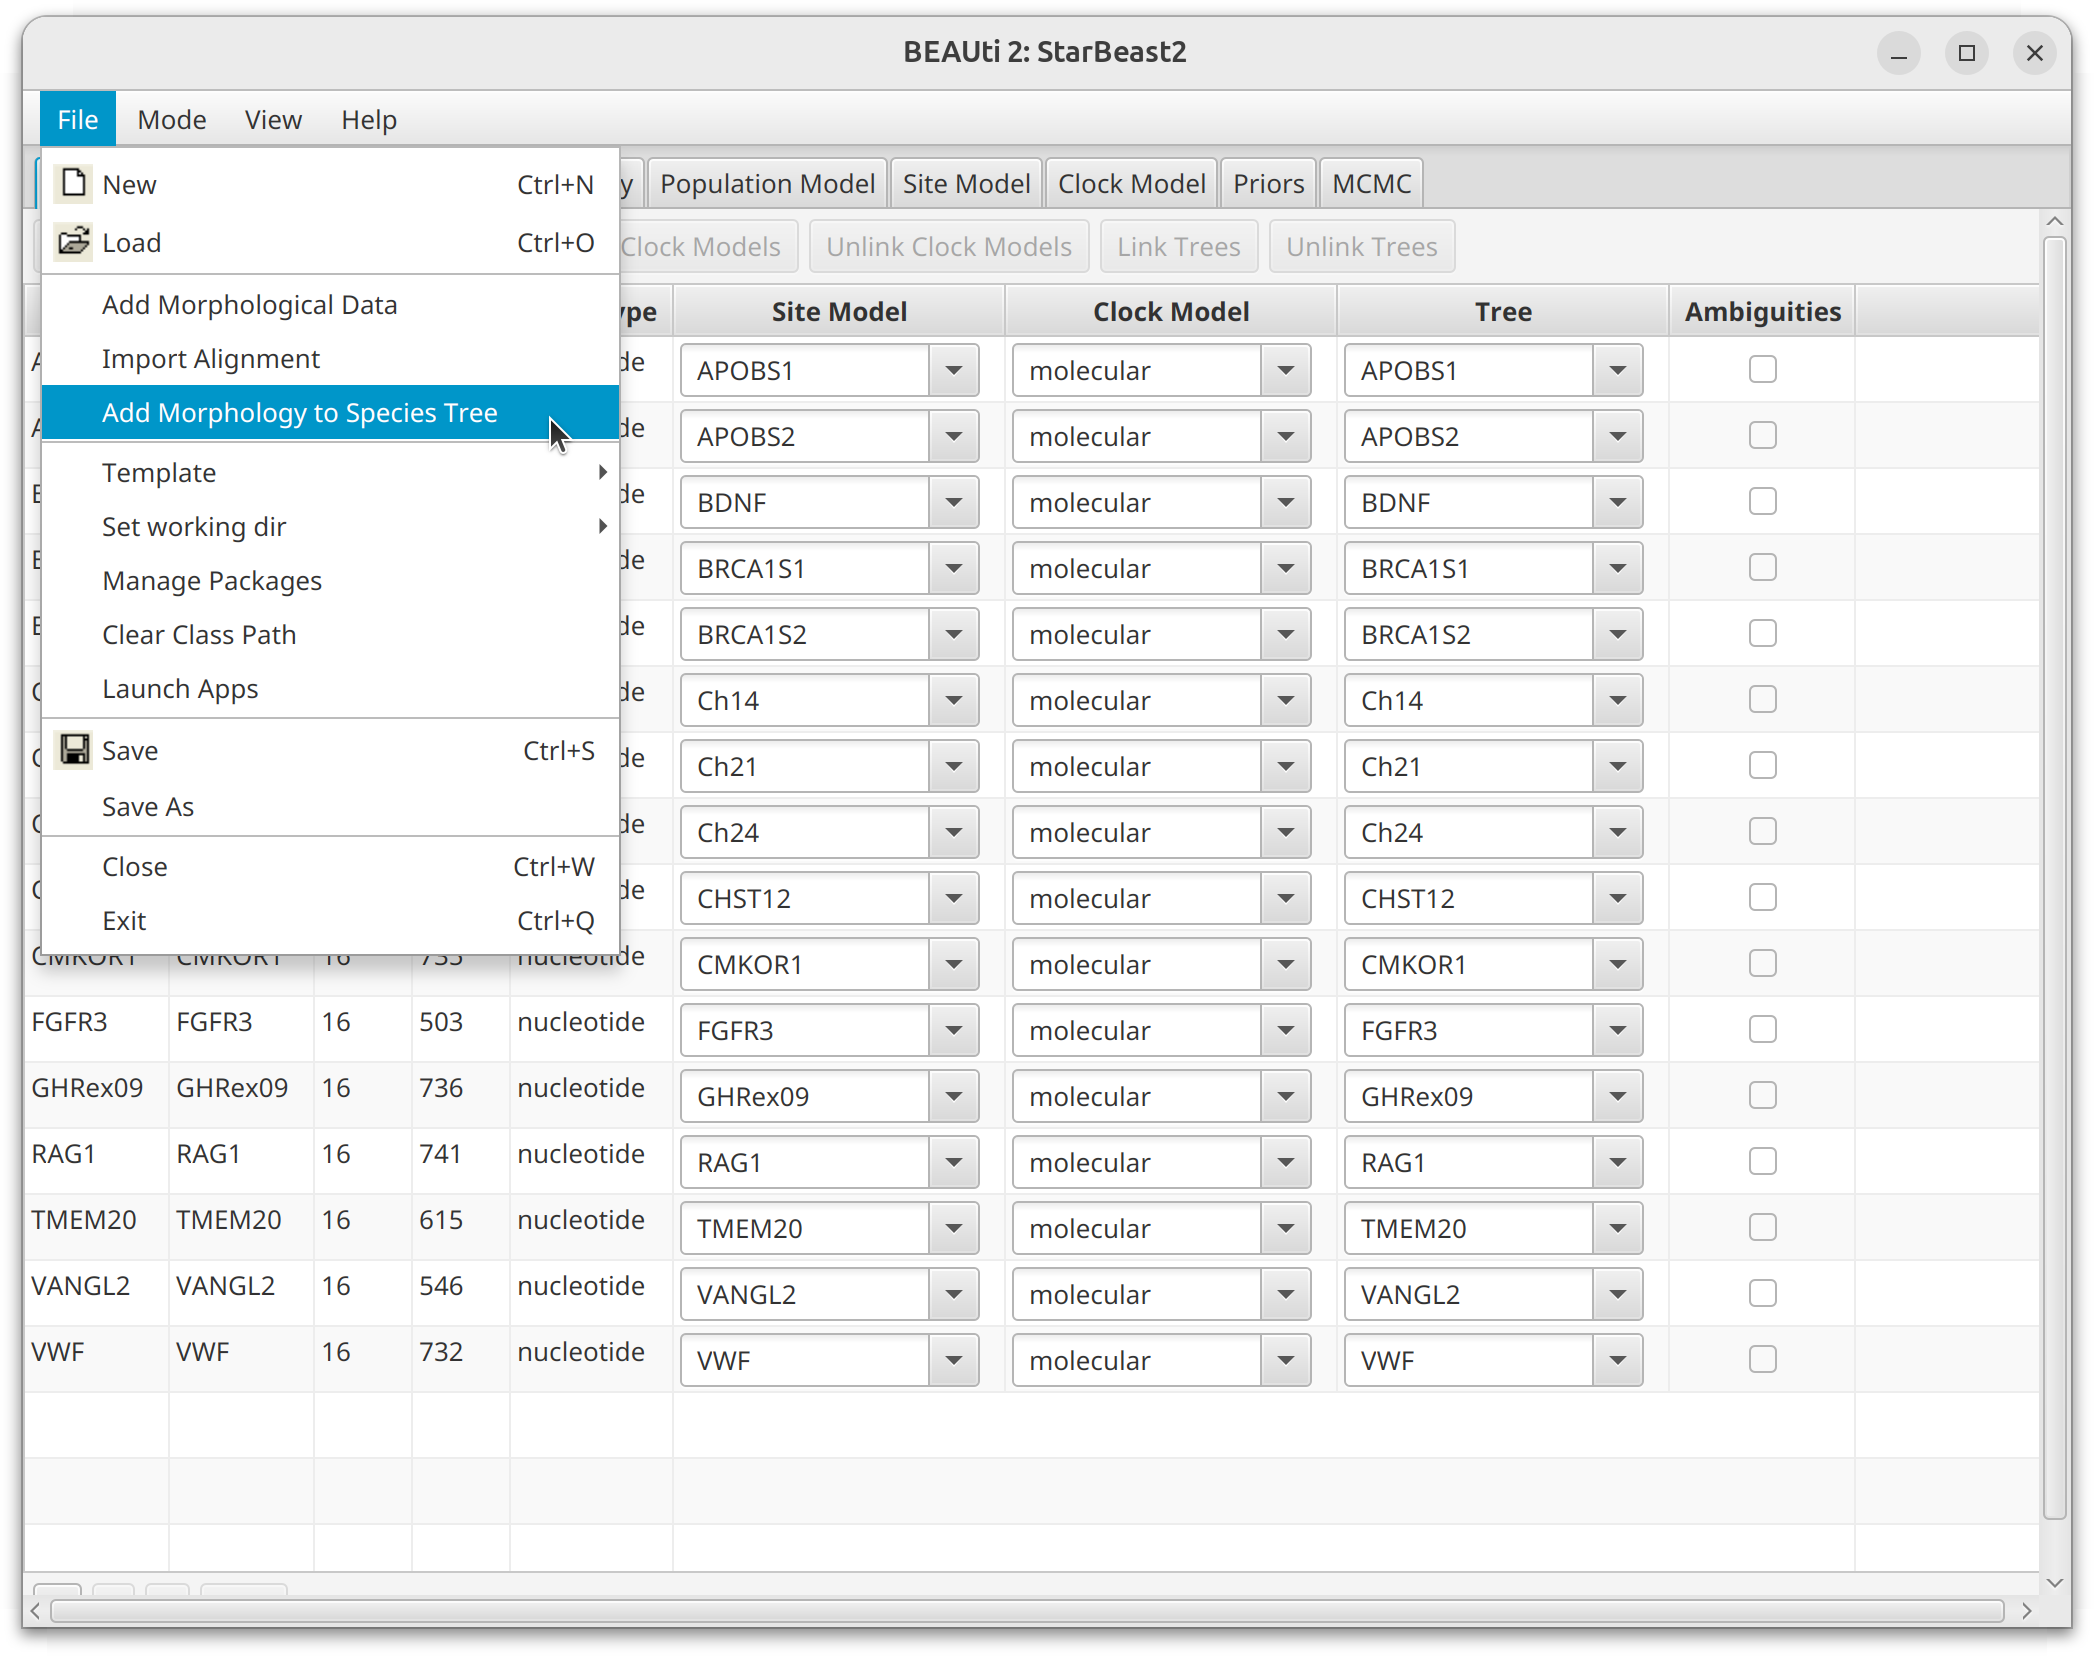
\includegraphics[width=0.8\textwidth]{figures/addMorphology.png}
\caption
{The option to add morphological data to the species tree}
\label{fig:addMorphology}
\end{figure}

Select Yes to condition on recording variable characters only (Mkv). Mkv is
used when only characters that vary between species have been included in the
character matrix, as is the case for this tutorial's data set. You
should now see four morphology partitions
(Figure~\ref{fig:morphologyPartitions}), one for each number of character
states. For example, morphology\_canis2 is for binary characters.

\begin{figure}[htb!]
\centering
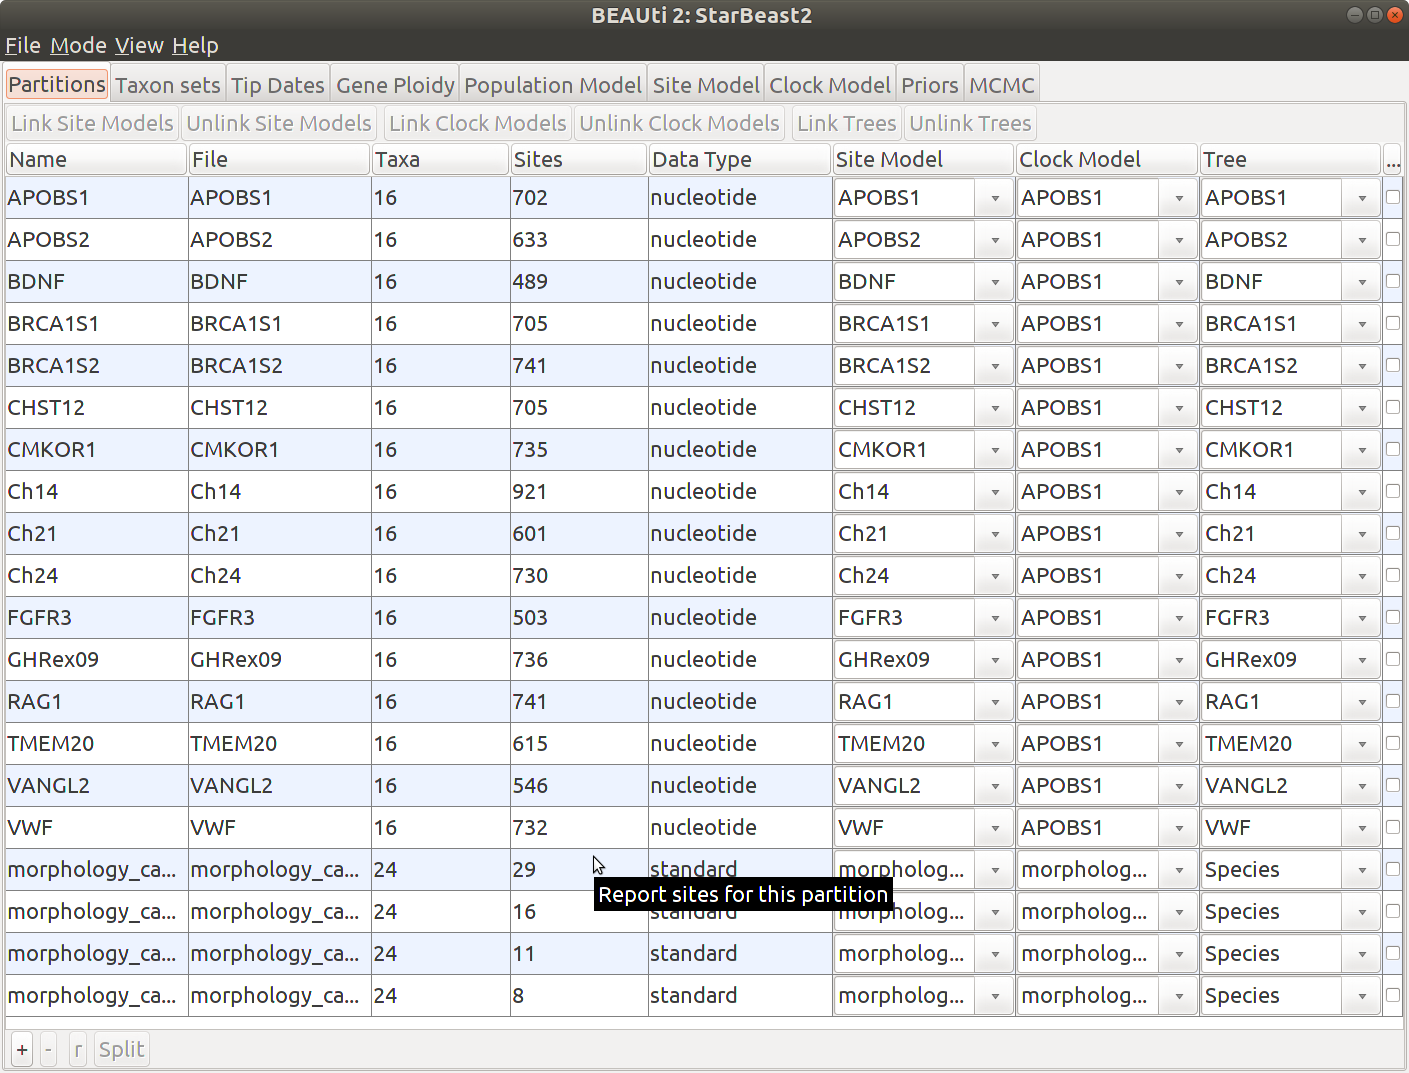
\includegraphics[width=0.8\textwidth]{figures/morphologyPartitions.png}
\caption
{After morphological data has been added to the species tree}
\label{fig:morphologyPartitions}
\end{figure}

\clearpage

Open the Tip Dates panel and enable ``Use tip dates''. Change
``Since some time in the past'' to ``before the present''. Click
on Auto-configure and select ``read from file''. Choose the
``tip\_dates\_canis.txt'' file in the data folder of the tutorial.
Click OK, and your tip dates should look like Figure~\ref{fig:tipDates}.

\begin{figure}[htb!]
\centering
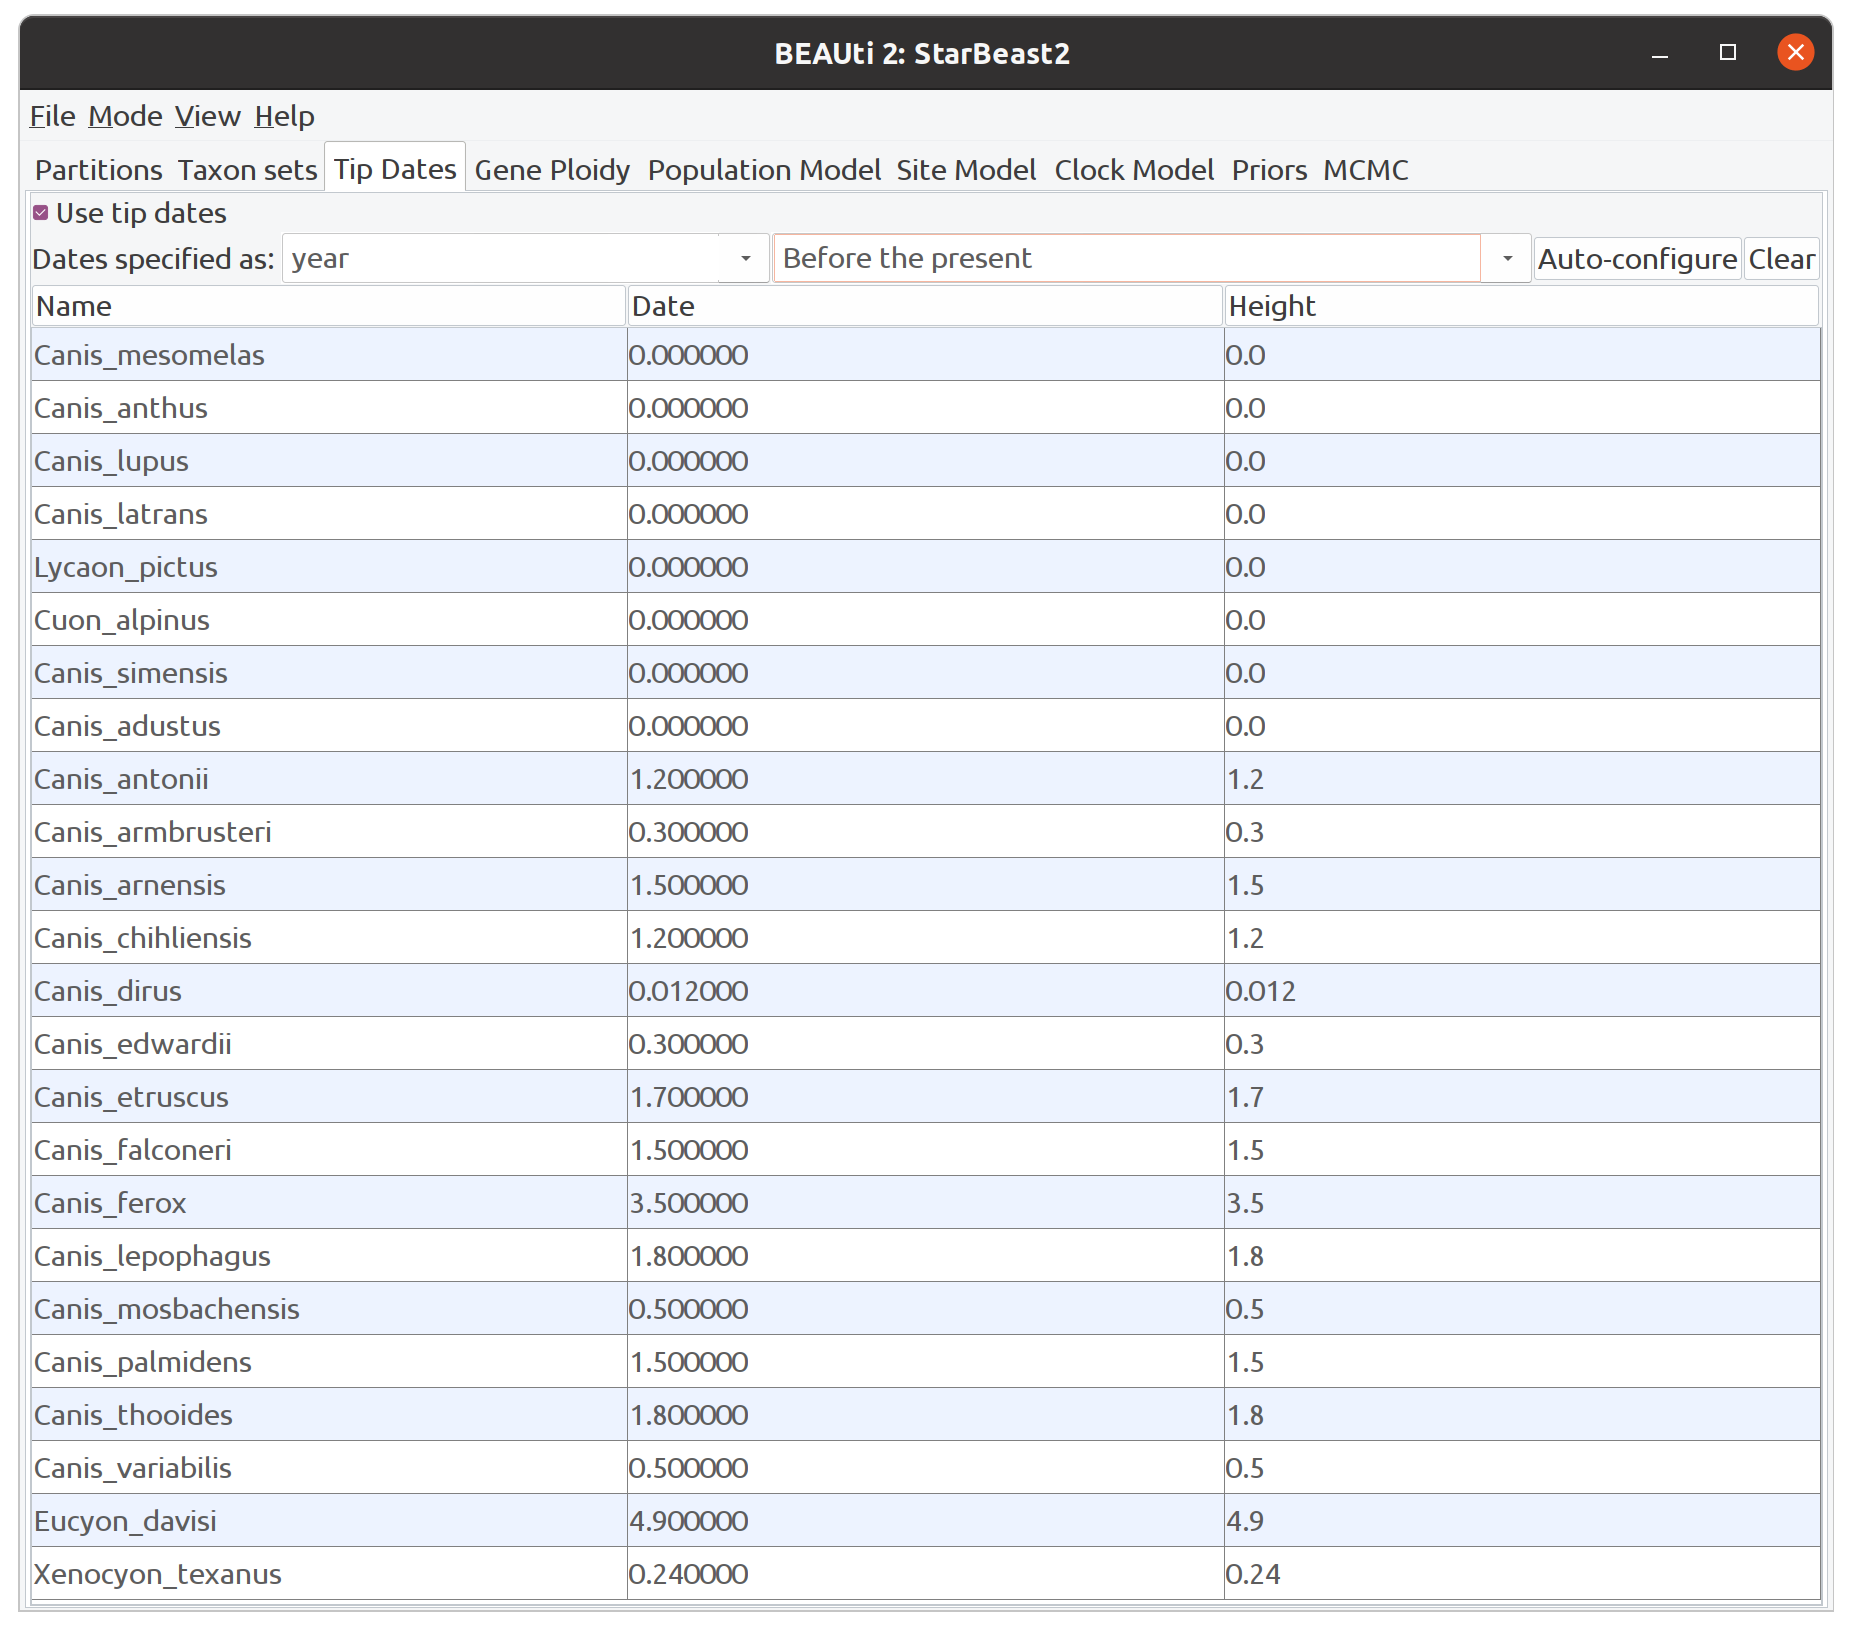
\includegraphics[width=0.8\textwidth]{figures/tipDates.png}
\caption
{Configured tip dates}
\label{fig:tipDates}
\end{figure}

Go to the Clock Model panel, and enable ``estimate'' for the
molecular clock (by default called APOBS1 after the first locus, although
this can be changed in the Partitions tab). Then select the morphological
data partition and enable ``estimate'' so that the morphological
clock rate will also be estimated (Figure~\ref{fig:estimateMorphClock}).
Make sure you have enabled ``estimate'' for \textbf{both} clocks, since we
are using fossil data to calibrate our tree.

\begin{figure}[htb!]
\centering
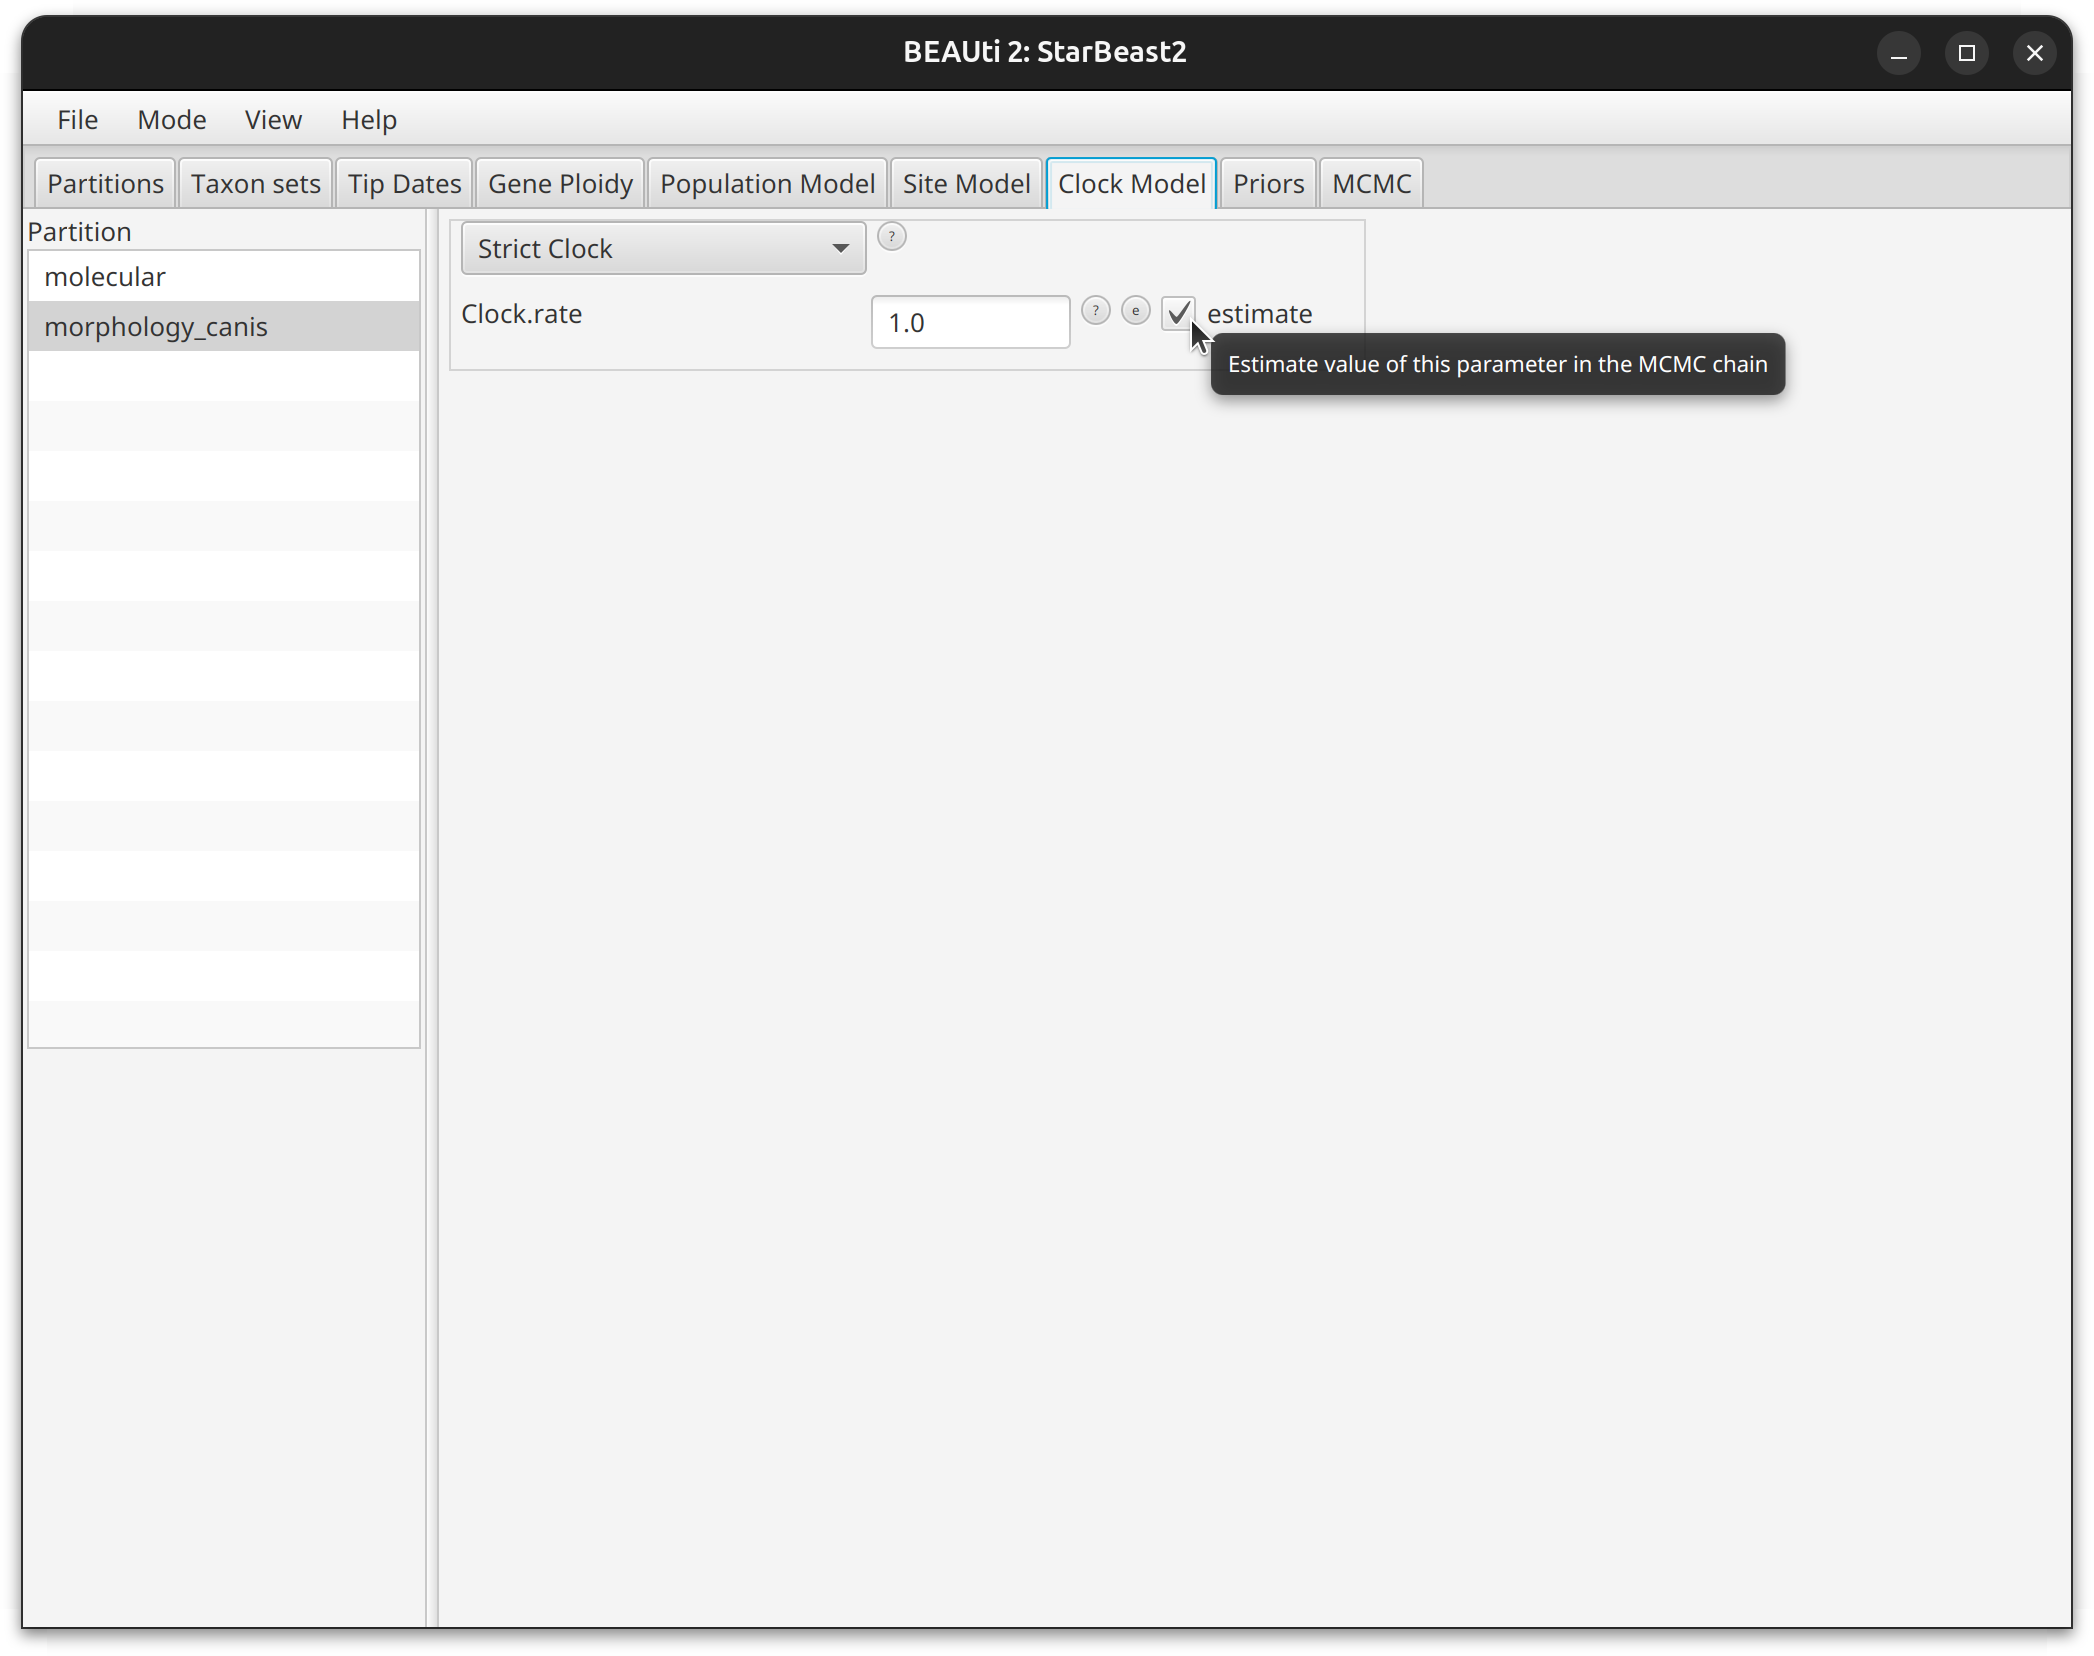
\includegraphics[width=0.8\textwidth]{figures/estimateMorphClock.png}
\caption
{Estimating the clock rates}
\label{fig:estimateMorphClock}
\end{figure}

Next, open the Priors panel and change the Tree prior from Yule to
``FBDModel''. Scroll down to the strictClockRate.c:molecular parameter,
and expand that prior. Change the mean to 0.001, the \textit{a priori}
molecular clock rate estimate from section~\ref{sec:speciesTree}. Leave
the standard deviation set at 1, a moderately informative prior that will
still allow the rate to be informed by the fossil data. Then
change the prior distribution for the strictClockRate.c:morphology\_canis
prior to 1/X (Figure~\ref{fig:clockPriors}). This is an improper,
uninformative prior so the inferred morphological clock rate will be
estimated solely from the data.

\begin{figure}[htb!]
\centering
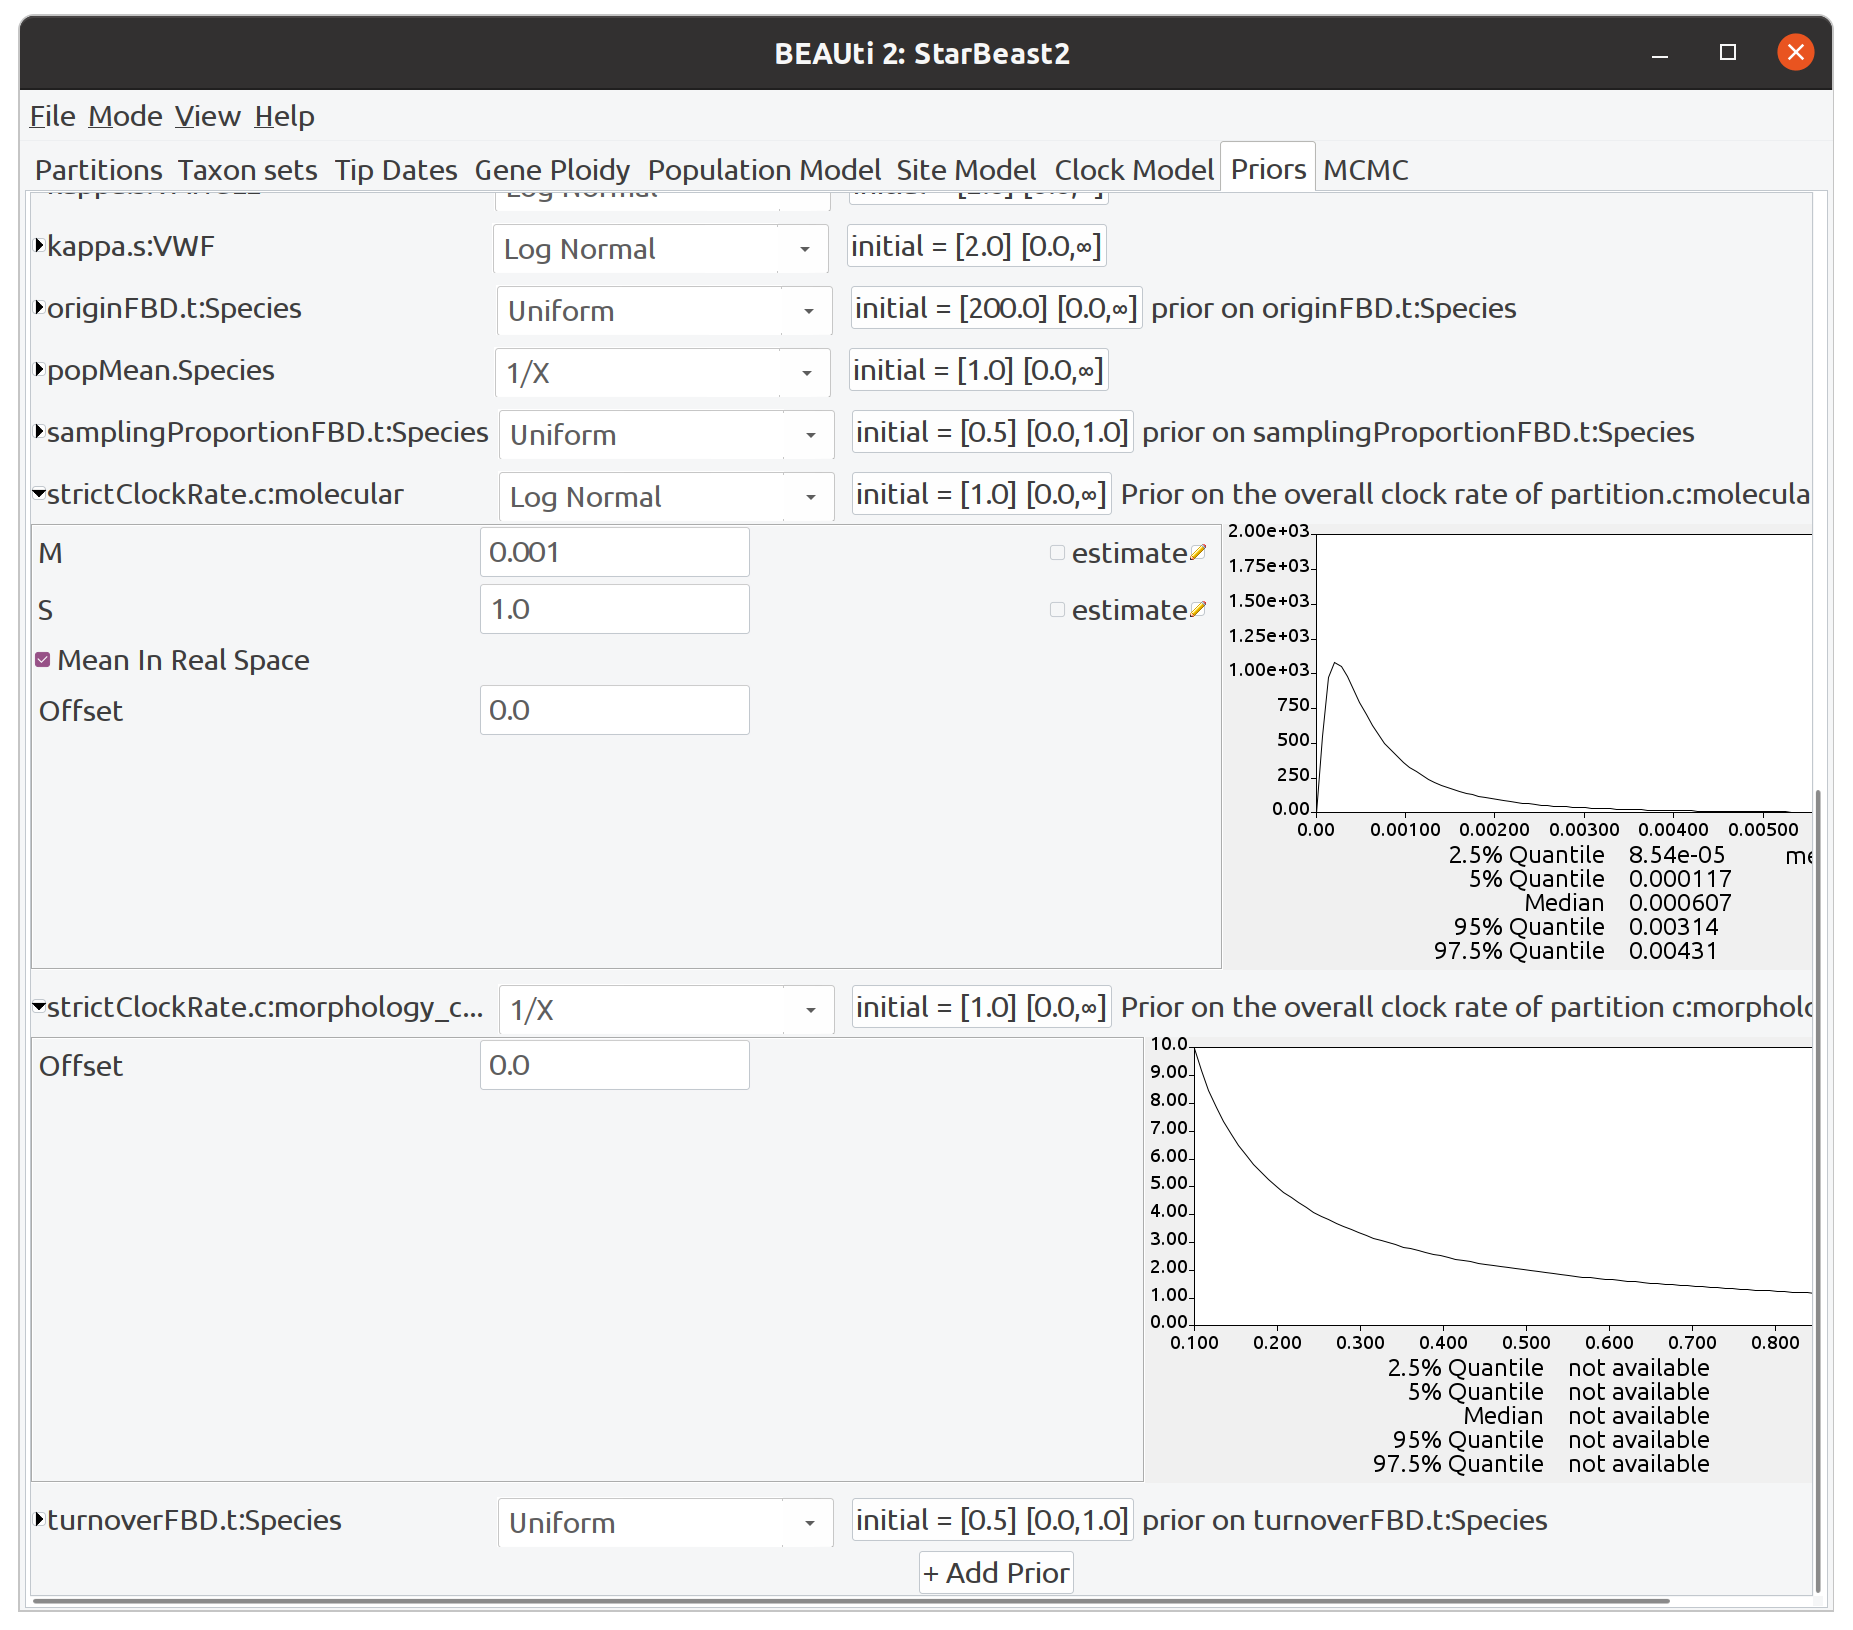
\includegraphics[width=0.8\textwidth]{figures/clockPriors.png}
\caption
{Configuring the clock prior distributions}
\label{fig:clockPriors}
\end{figure}

\newpage{}

The FBD-MSC model is quite complex and requires very long chains for
reliable sampling. Open the MCMC tab and change the chain length to 200
million. We will need to reduce the sampling rate so that the output files remain
managably small, so change the Store Every value to 50,000. Expand the
tracelog, speciesTreeLogger, screenlog and every gene tree log, and set the
Log Every value to 50,000 for each of them. This will limit the number of
samples to 4,000 in each log file (Figure~\ref{fig:fbdChainLength}).

\begin{figure}[htb!]
\centering
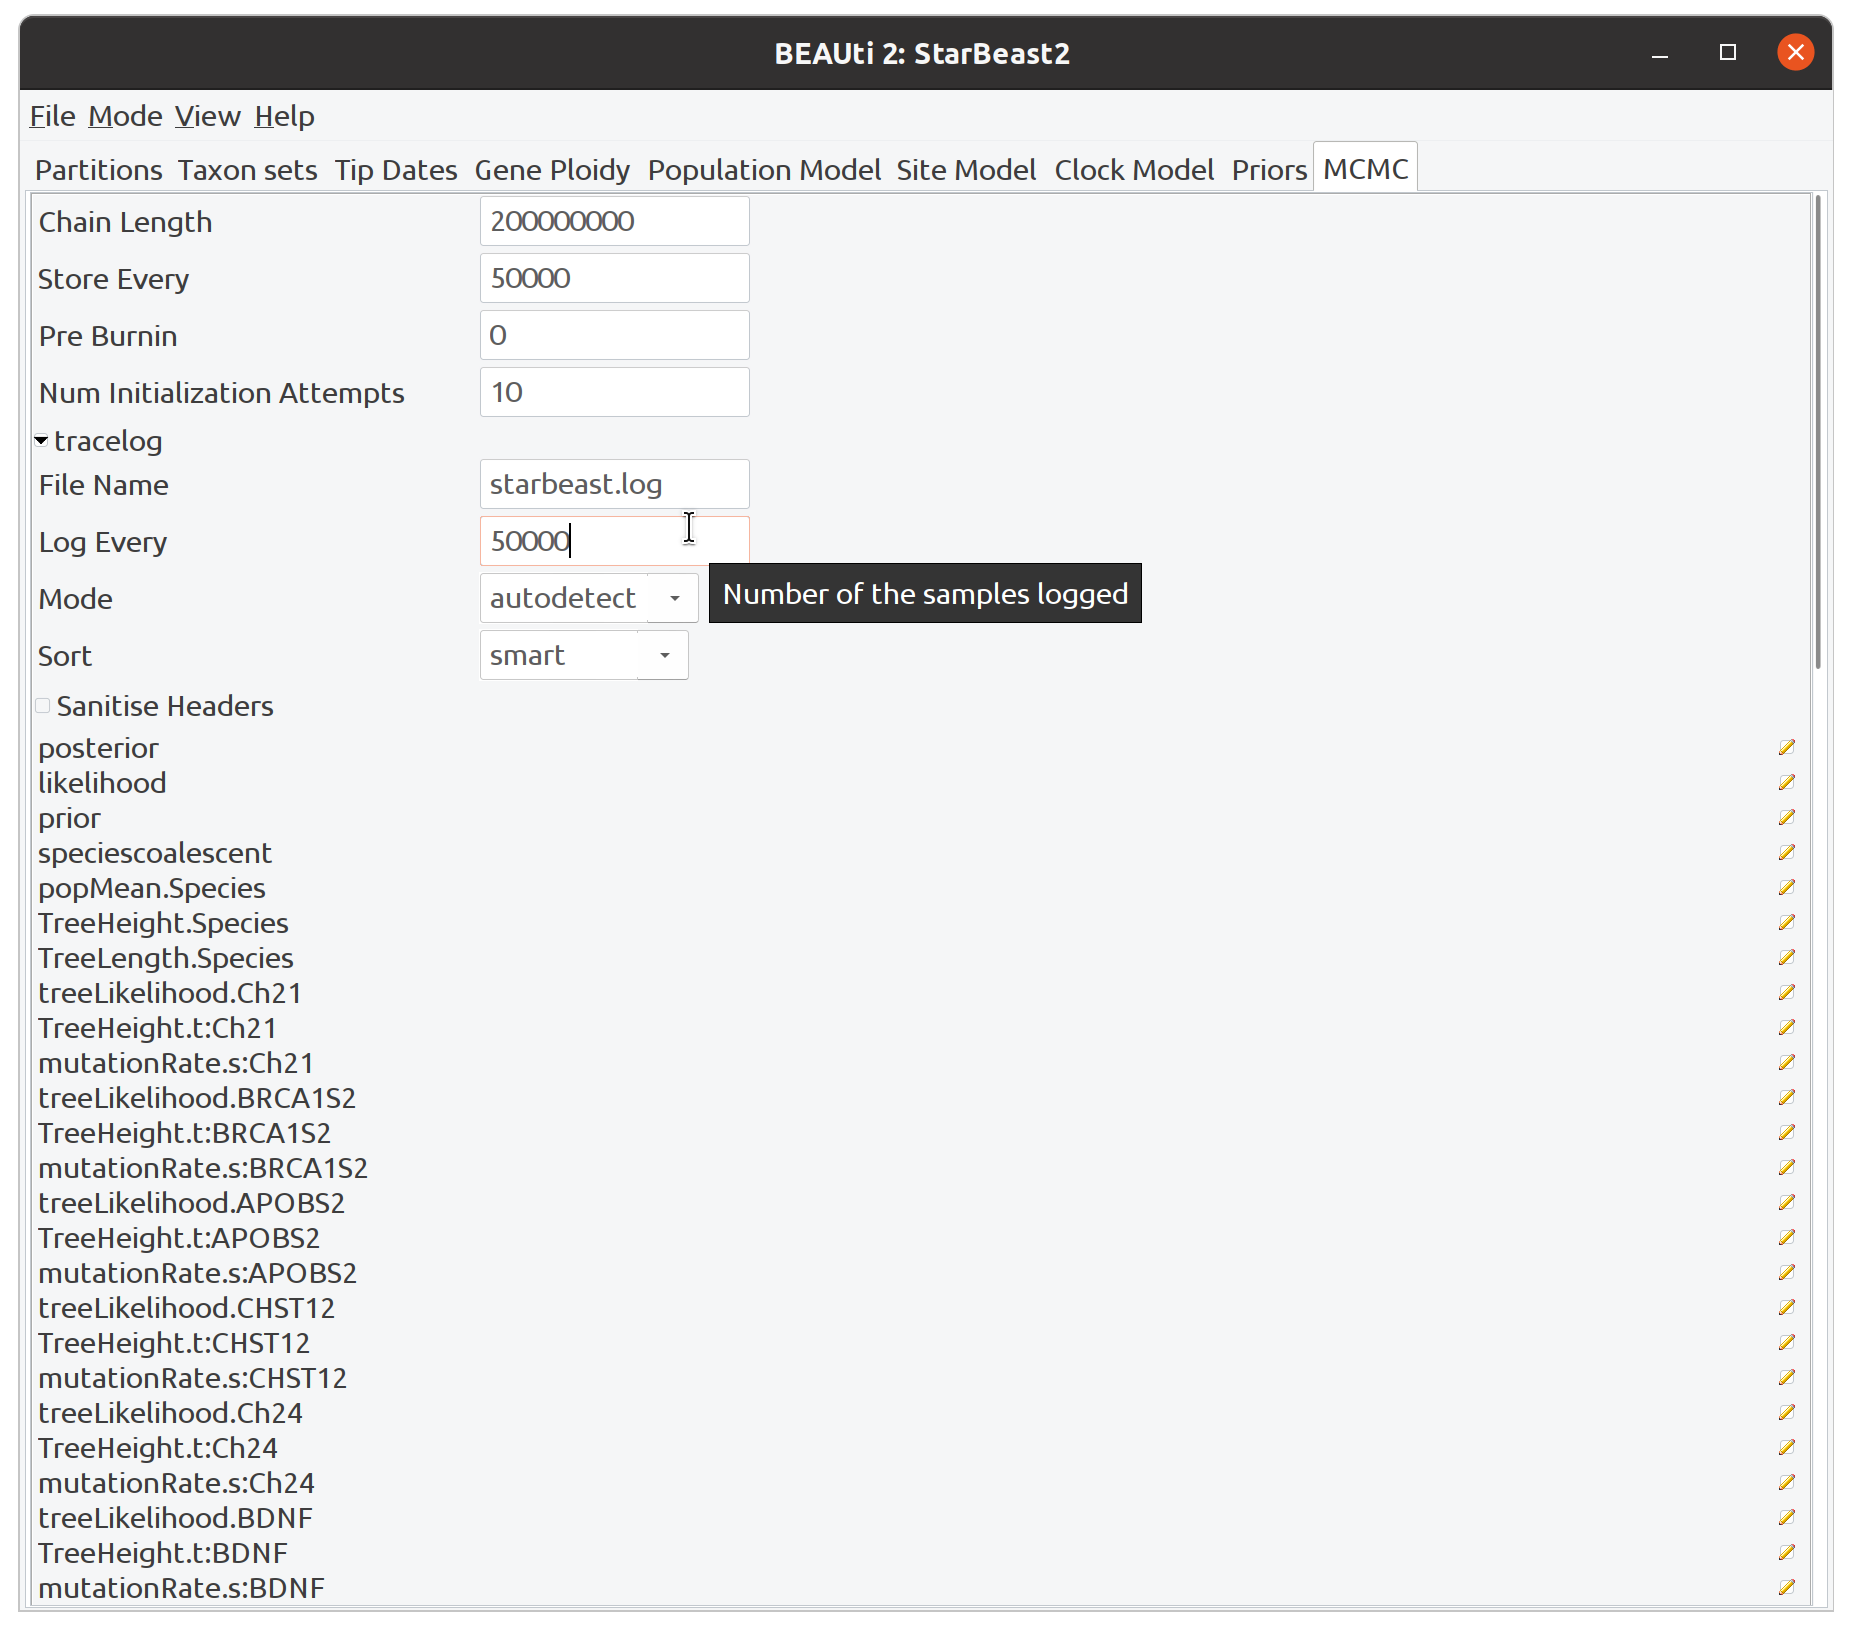
\includegraphics[width=0.8\textwidth]{figures/fbdChainLength.png}
\caption
{Setting a very long chain length}
\label{fig:fbdChainLength}
\end{figure}

Save the XML file in the folder you created for this analysis, and name it
something like ``CanisFBD.xml''. Run the MCMC chain by opening the XML file in
BEAST, or running it from the command line as in
subsection~\ref{subsec:runningBEAST}. The chain will take about 2 hours to
finish, depending on the speed of your computer.

After BEAST has finished, open the ``starbeast.log'' file in Tracer to check
on the ESS values. Select the strictClockRate.c:molecular parameter
(Figure~\ref{fig:strictClockRate}). The 95\% HPD interval for this parameter
spans approximately 0.0005 to 0.0013 substitutions per site per million years,
in agreement with the \textit{a priori} rate of 0.001.

\begin{figure}[htb!]
\centering
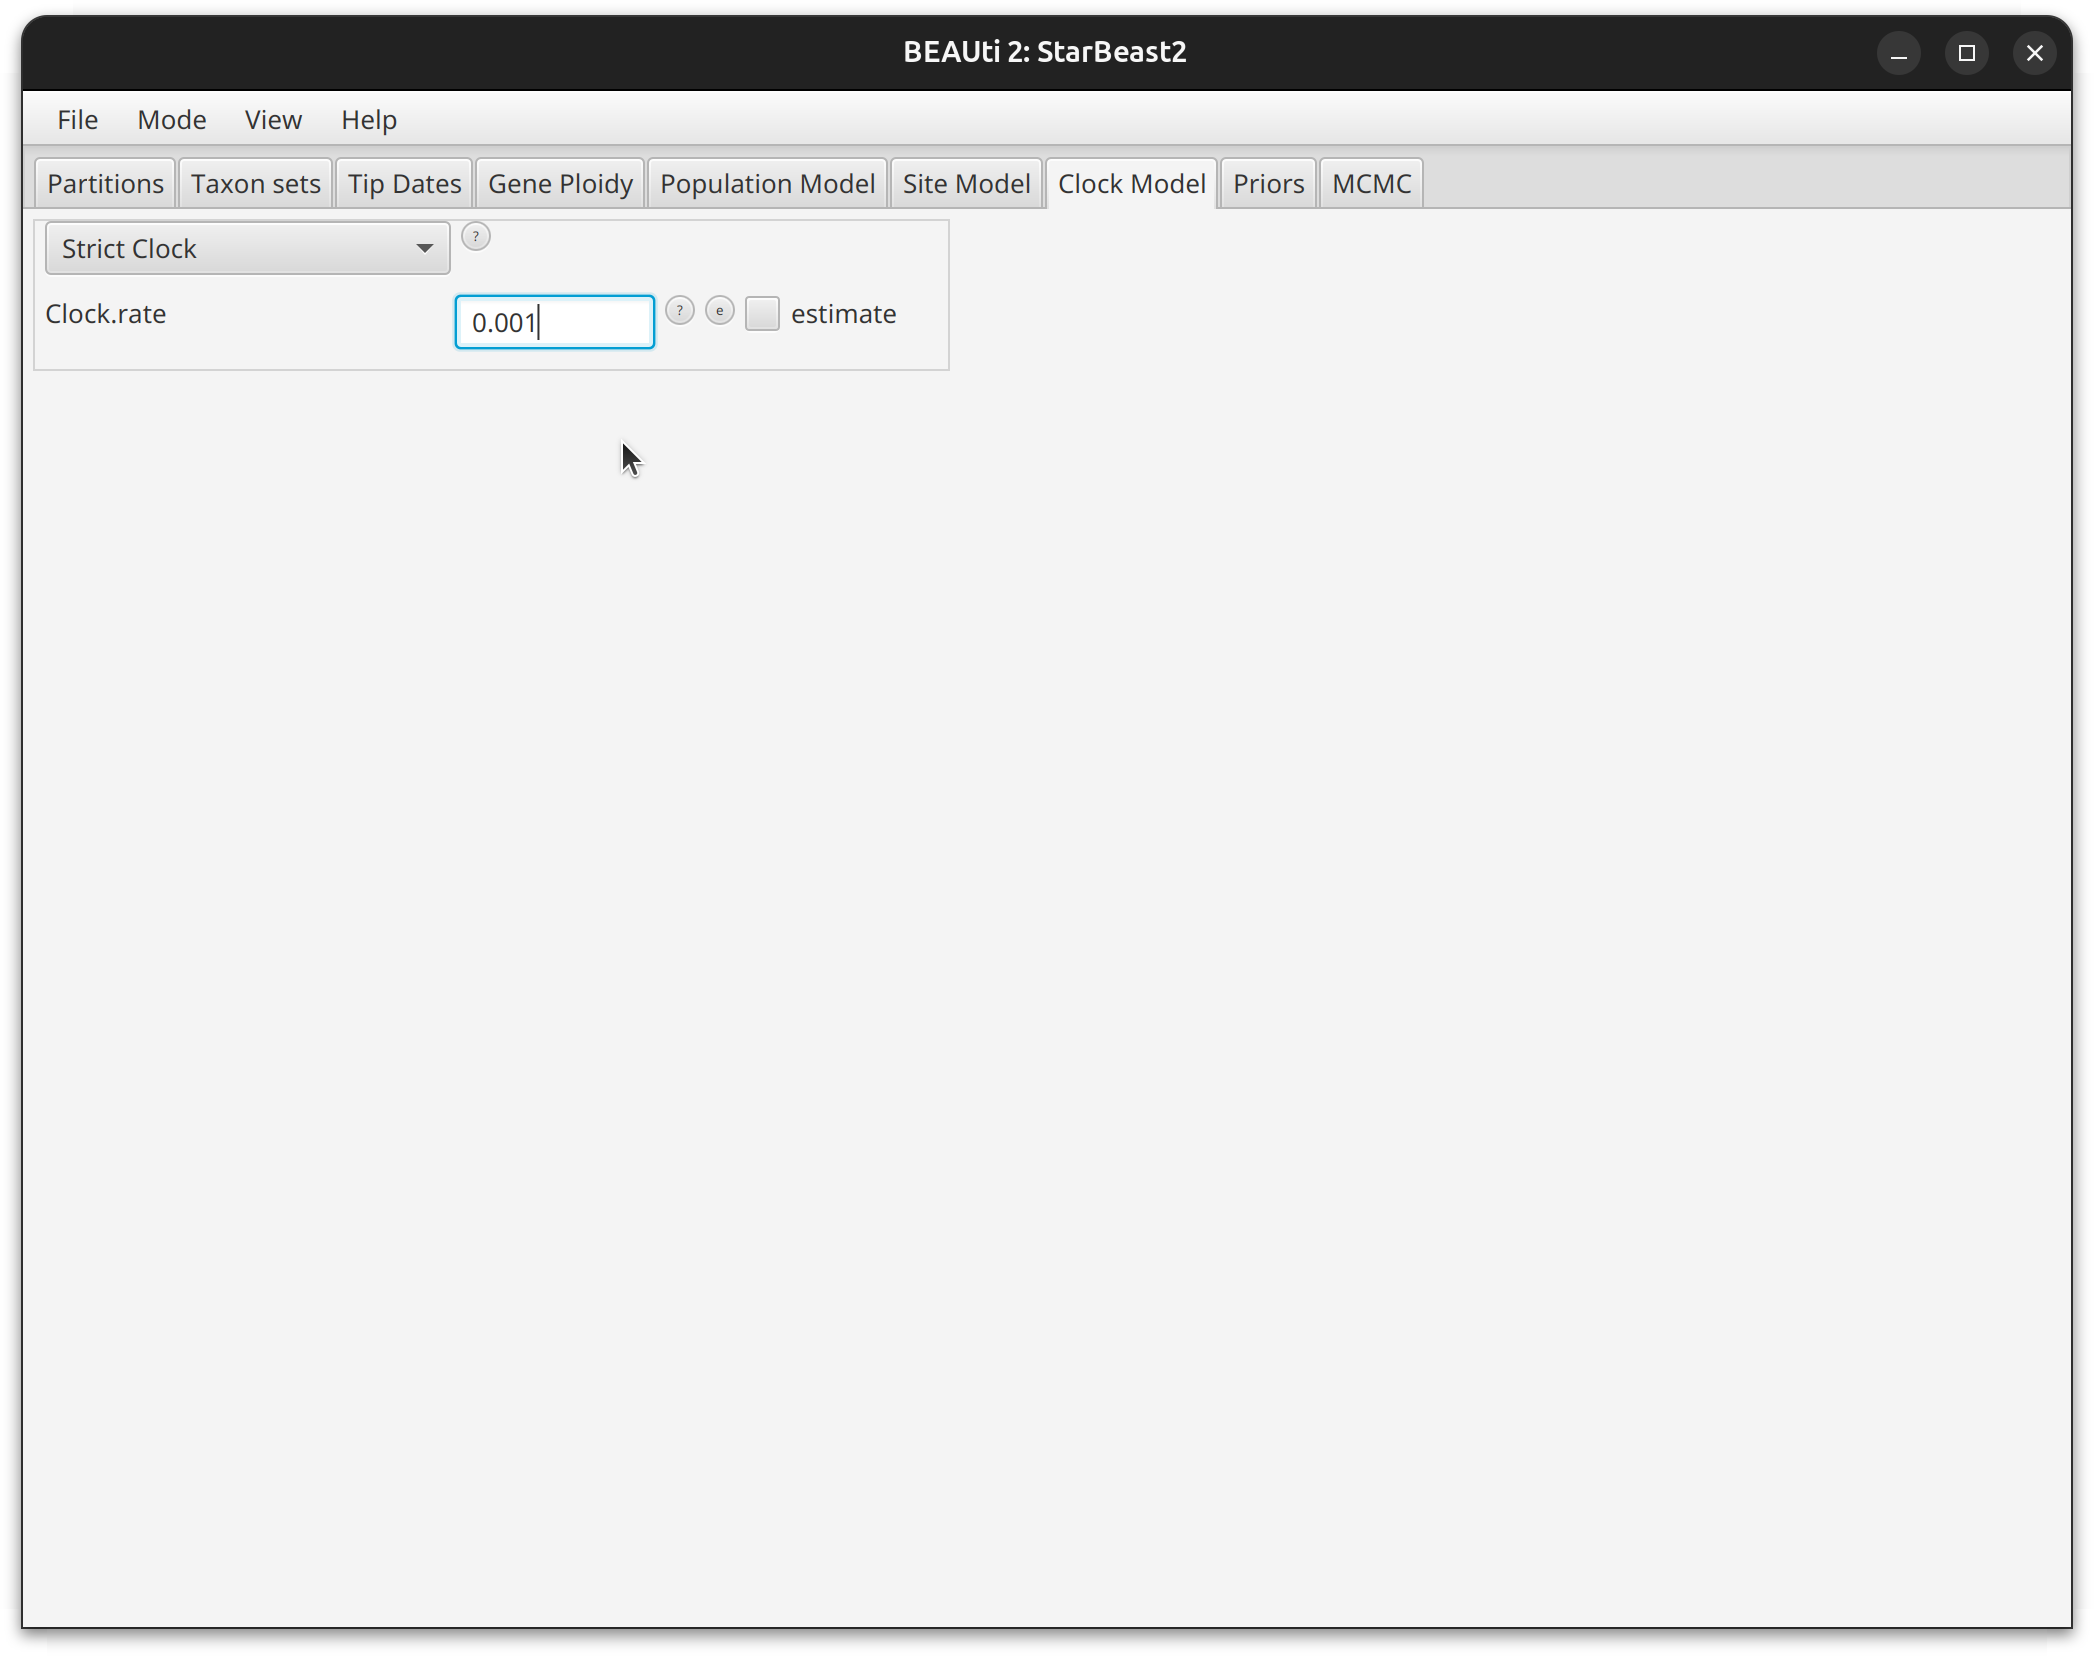
\includegraphics[width=0.8\textwidth]{figures/strictClockRate.png}
\caption
{The posterior estimate of the molecular clock rate}
\label{fig:strictClockRate}
\end{figure}

Start the DensiTree app again, and then open the ``species.trees'' file. Under
the Show panel, enable the Root Canal tree to get an idea of the most
plausible species tree. Then open the Grid panel, and enable the full grid.
Compared with the fixed clock analysis (Figure~\ref{fig:densitree}), the
divergence time between \textit{Canis lupus} and \textit{Canis latrans} is a
little older, and the age of the MRCA of extant species is a little younger
(Figure~\ref{fig:densitreeSA}).

\begin{figure}[htb!]
\centering
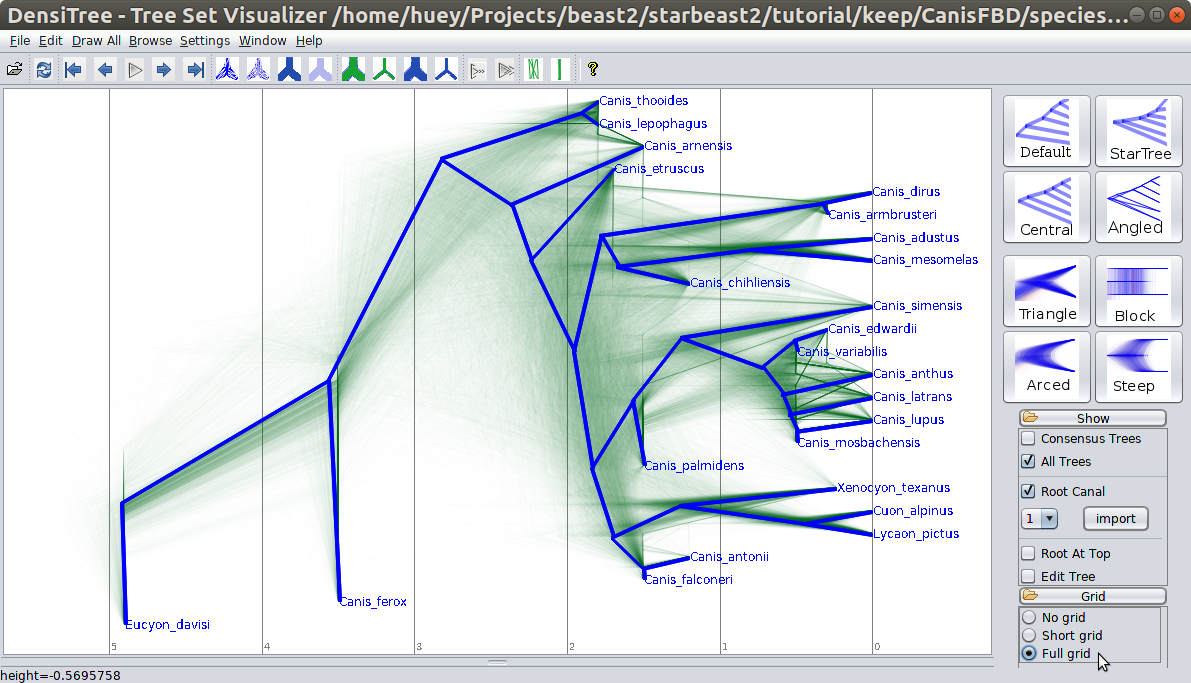
\includegraphics[width=0.8\textwidth]{figures/densitreeSA.png}
\caption
{Cloud of FBD-MSC species trees}
\label{fig:densitreeSA}
\end{figure}

\clearpage

Open the Tree Annotator app included with BEAST2, and set the burnin
percentage to 10. Trees inferred by the FBD-MSC model as implemented in
StarBEAST2 can include sampled ancestors \parencite{Gavryushkina2014}, which are
incompatible with Common Ancestor heights \parencite{Heled2013} as implemented in
Tree Annotator. So in order to generate a summary tree, change ``Node heights'' to
``Mean heights'' (Figure~\ref{fig:treeAnnotatorMeanHeights}). Choose the
``species.trees'' file as the input file, and specify the output file to be
something sensible like ``summary.tree'', then click Run.

\begin{figure}[htb!]
\centering
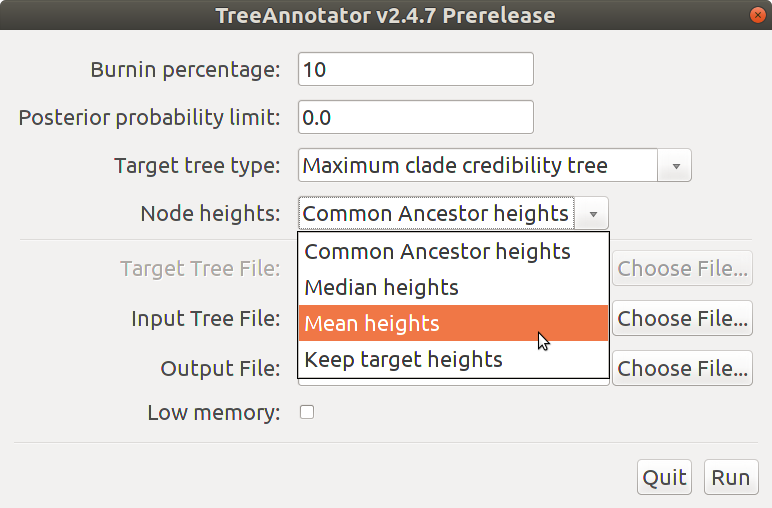
\includegraphics[width=0.5\textwidth]{figures/treeAnnotatorMeanHeights.png}
\caption
{Running Tree Annotator for sampled ancestor trees}
\label{fig:treeAnnotatorMeanHeights}
\end{figure}

Start FigTree and open the summary tree file you have just created. Enable
Node Labels, and expand the Node Labels panel. Choose ``posterior'', and set
the number of significant digits to 2. Now the posterior support for each
clade will be displayed next to each node (Figure~\ref{fig:figtreeFBD}).

\clearpage

\begin{figure}[htb!]
\centering
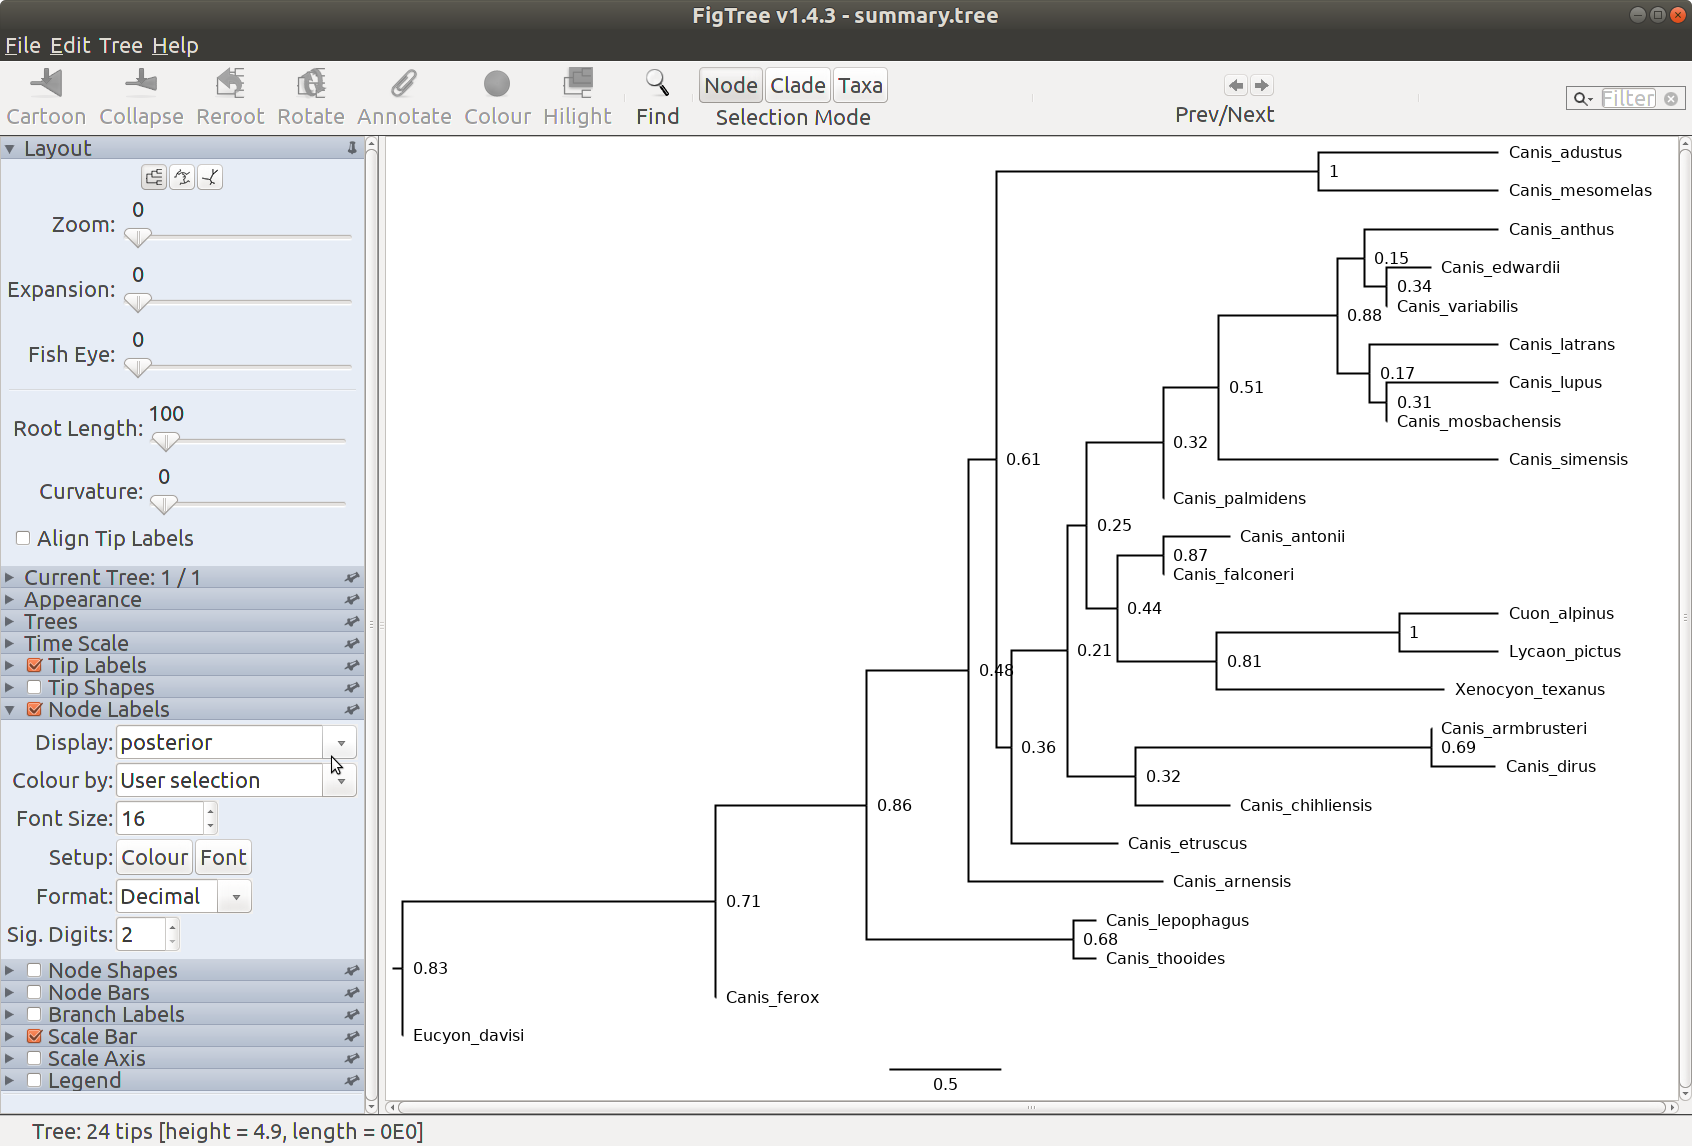
\includegraphics[width=0.8\textwidth]{figures/figtreeFBD.png}
\caption
{Showing posterior support for clades in FigTree}
\label{fig:figtreeFBD}
\end{figure}

The tree topology is similar to the fixed clock analysis
(Figure~\ref{fig:figtree}), except that \textit{Cuon alpinus} and
\textit{Lycaon pictus} are now a clade with 100\% support. A disagreement
between molecular data which contradicts this clade and morphological
data which supports it has been reported previously \parencite{Zrzavy2004}. This shows
how morphological characters and fossil data can influence species tree
estimates.

\clearpage

\section{Wrapping up}

That concludes the tutorial. One final note; when runnning any MCMC method, it
is possible than the chain has gotten stuck in a region of parameter space
with high local probability. So for any kind of analysis intended for
publication, it is a good idea to run at least two MCMC chains. Open both
chains in Tracer, and check that the traces for the logged statistics and
parameters have the same distributions.

\printbibliography

\end{document}
